\documentclass[dvipdfmx]{jsarticle}
\usepackage{tikz}
\usepackage{bbm}
\usepackage{amsmath,amssymb}
\usepackage{url}
\usetikzlibrary{matrix,arrows}

\newcommand{\cat}[1]{\mathbbm{#1}}
\newcommand{\arrow}{\rightarrow}
\newcommand{\functor}[3]{#1:\cat{#2}\arrow \cat{#3}}
\newcommand{\nat}[3]{#1:#2\Rightarrow #3}
\newcommand{\natf}[5]{#1:#2\Rightarrow #3:\cat{#4}\arrow \cat{#5}}
\newcommand{\tuple}[1]{\langle #1\rangle}
\newcommand{\objr}[1]{\mathrm{Obj}(#1)}
\newcommand{\obj}[1]{\mathrm{Obj}(\cat{#1})}
\newcommand{\mor}[3]{#1:#2\arrow #3}
\newcommand{\dom}{\mathrm{dom}}
\newcommand{\cod}{\mathrm{cod}}
\newcommand{\arset}[3]{\cat{#1}(#2,#3)}
\newcommand{\arsetr}[3]{#1(#2,#3)}
\newcommand{\pcobj}[1]{[#1]}
\newtheorem{proof}{証明}[section]
\newtheorem{prop}{命題}[section]
\newtheorem{define}{定義}[section]
\numberwithin{proof}{subsection}
\numberwithin{prop}{subsection}
\numberwithin{define}{subsection}
\begin{document}
	\title{圏論入門}
	\maketitle
	\tableofcontents
	\section{はじめに}
	圏論は抽象代数学で生まれ、現在では代数学、幾何学、数学基礎論や、計算機科学、言語学、認知科学、哲学などにも応用されている数学の一分野である。
	本資料は数学基礎論や計算機科学で特に使われるデカルト閉圏を中心に解説していく。
	また他の入門書の差別化として、できるだけ議論や具体例を圏論の中で完結するようにしている。
	\section{圏と公理}

	\begin{define}
		ある圏$\cat{C}$は以下で定義される対象集合と、任意の二対象に対する射の集合の全体、合成の演算の三つ組\[(\obj{C},\prod\limits_{A,B}^{\obj{C}}\arset{C}{A}{B},\circ)\]によって定義する。また圏は以下に示す公理を満たさなければならない。
		\begin{quote}
			\begin{description}
			\item[対象] 対象の集合$\obj{C}\ni A,B,C...$
			\item[射] 任意の対象$A,B$における射の集合$\arset{C}{A}{B}\ni f,g,h...$

			このような射の集合は任意の対象の組み合わせごとに存在する。
			また$f\in\arset{C}{A}{B}$を$\mor{f}{A}{B}$と書く。このとき$f$に対する$A$をドメイン、$B$をコドメインと呼び、射から対象への二つの演算$\dom,\cod$を用い$\dom(f)=A$、$\cod(f)=B$と表す。

			ある対象$A,B,C$、ある射$\mor{f}{A}{B}$、$\mor{g}{A}{C}$、$\mor{h}{C}{B}$について考えるとき、以下のような図式を用いて説明を行う。
			\begin{center}
				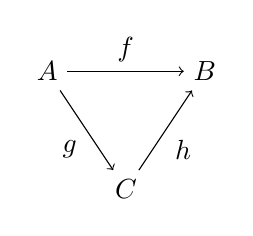
\begin{tikzpicture}[auto]
					\node (a) at (0, 0) {$A$};
					\node (b) at (2, 0) {$B$};
					\node (c) at (1, -1.5) {$C$};
					\draw[->] (a) to node {$f$}(b);
					\draw[->] (a) to node[swap] {$g$}(c);
					\draw[->] (c) to node[swap] {$h$}(b);
				\end{tikzpicture}
			\end{center}

			\item[射の合成]~\\ ある射$f,g$が$\cod(f)=\dom(g)$を満たす、つまり$\mor{f}{X}{A}$、$\mor{g}{A}{Y}$であるようなとき、合成射$\mor{g\circ f}{X}{Y}$が定まる。
			射をつなげる、という直感に反して合成射の射の順序が射の向きと逆であることに注意してほしい。

			射$h,g$の合成$h\circ g$は次のように表せる。
			また対象$A$と対象$B$の間の射は一つとは限らないので、必ずしも$h\circ g=f$が成り立つわけではない。
			\begin{center}
				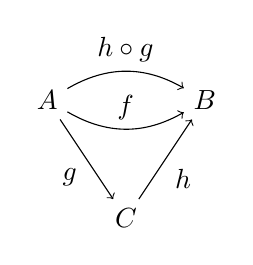
\begin{tikzpicture}[auto]
					\node (a) at (0, 0) {$A$};
					\node (b) at (2, 0) {$B$};
					\node (c) at (1, -1.5) {$C$};
					\draw[->] (a) to[bend right=30] node {$f$}(b);
					\draw[->] (a) to[bend right=-30] node {$h\circ g$}(b);
					\draw[->] (a) to node[swap] {$g$}(c);
					\draw[->] (c) to node[swap] {$h$}(b);
				\end{tikzpicture}
			\end{center}
			このような操作は任意の対象$A,B,C$における二項演算\[\mor{\circ}{\arset{\cat{C}}{B}{C}\times\arset{\cat{C}}{A}{B}}{\arset{\cat{C}}{A}{C}}\]
			で表せる。
			\item[恒等射の存在] 恒等射と呼ばれる特別な射$\mor{id_A}{A}{A}$が任意の対象に存在する。
			\begin{center}
				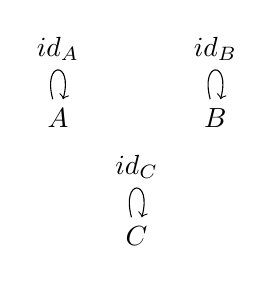
\begin{tikzpicture}[auto]
					\node (a) at (0, 0) {$A$};
					\node (b) at (2, 0) {$B$};
					\node (c) at (1, -1.5) {$C$};
					\draw[->,loop above ,looseness=10] (a) to node{$id_A$}(a);
					\draw[->,loop above ,looseness=10] (b) to node{$id_B$}(b);
					\draw[->,loop above ,looseness=10] (c) to node{$id_C$}(c);
				\end{tikzpicture}
			\end{center}
			\item[結合律] 結合則$h\circ (g\circ f)=(h\circ g)\circ f$が合成可能な任意の射$f,g,h$で成り立つ。
				\begin{center}
				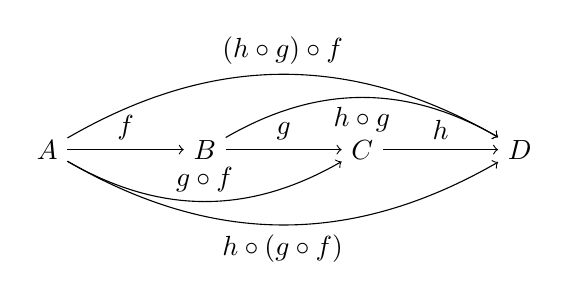
\begin{tikzpicture}[auto]
					\node (a) at (0, 0) {$A$};
					\node (b) at (2, 0) {$B$};
					\node (c) at (4, 0) {$C$};
					\node (d) at (6, 0) {$D$};
					\draw[->] (a) to node {$f$}(b);
					\draw[->] (b) to node {$g$}(c);
					\draw[->] (c) to node {$h$}(d);
					\draw[->] (a) to[bend right=30] node {$g\circ f$}(c);
					\draw[->] (a) to[bend right=30] node[swap] {$h\circ(g\circ f)$}(d);
					\draw[->] (b) to[bend left=30] node[swap] {$h\circ g$}(d);
					\draw[->] (a) to[bend left=30] node {$(h\circ g)\circ f$}(d);
				\end{tikzpicture}
			\end{center}
			\item[単位元律]~\\ 任意の対象$A$と対応する恒等射$\mor{id_A}{A}{A}$、任意の射$\mor{f}{X}{A}$、$\mor{g}{A}{Y}$において\[id_A\circ f=f,\ g\circ id_A=g\]が成り立つ。

			恒等射をある射に合成しても、合成する前の射と等しくなることから、直感的に恒等射は何も行わない射のように考えられる。

			\begin{center}
				\begin{tikzpicture}[auto]
					\node (x) at (0, 0) {$X$};
					\node (a) at (2, 0) {$A$};
					\node (y) at (4, 0) {$Y$};
					\draw[->] (x) to node {$f$}(a);
					\draw[->,loop above, looseness=20] (a) to node {$id_A$}(a);
					\draw[->] (a) to node {$g$}(y);
				\end{tikzpicture}
				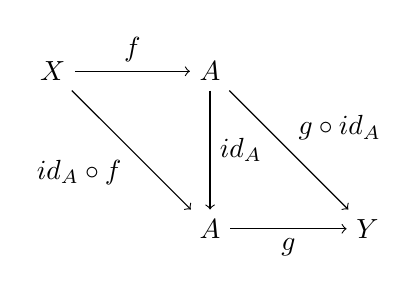
\begin{tikzpicture}[auto]
					\node (a) at (0, 0) {$X$};
					\node (b) at (2, 0) {$A$};
					\node (b') at (2, -2) {$A$};
					\node (c) at (4, -2) {$Y$};
					\draw[->] (a) to node {$f$}(b);
					\draw[->] (b) to node {$id_A$}(b');
					\draw[->] (b') to node[swap]  {$g$}(c);
					\draw[->] (a) to node[swap]  {$id_A\circ f$}(b');
					\draw[->] (b) to node {$g\circ id_A$}(c);
				\end{tikzpicture}
			\end{center}
		\end{description}
			\end{quote}
	\end{define}

	次に圏の例として集合の圏を挙げる。
	\begin{define}[集合の圏]
		圏$\cat{Set}$を以下の要素から構成する。
		\begin{quote}
			\begin{description}
				\item[対象] $\obj{Set}$を小さな集合の集合とする。

				「小さい」は自己言及を避けるための条件であり、実際に$\obj{Set}$は大きい集合となるため$\obj{Set}$には含まれない。
				\item[射] 二対象$A,B$に対する射集合$\arset{Set}{A}{B}$を小さな集合$A$から小さな集合$B$への写像の集合$\arset{Set}{A}{B}$とする。

				また紛らわしい場合を除いて小さい集合を集合と呼ぶことにする。

				集合の圏では一般的な圏とは違い、対象を集合として元をとることができる。
				そして同対象間に射が二つあったとき、二つの写像が等しいかどうかを元の対応関係で確かめることができる。
				つまり、二つの写像$\mor{f,g}{A}{B}$と集合$A$の任意の元$a$に対して、\[f(a)=g(a)\]ならば$f=g$が成り立つ、ということである。以降は元の対応関係を用いて集合の圏の射である写像を定義していく。

				\item[射の合成]  二つの写像$\mor{f}{A}{B}$、$\mor{g}{B}{C}$の合成写像$\mor{g\circ f}{A}{C}$を$A$の任意の元$a$に対して\[(g\circ f)(a)=g(f(a))\]となるように定義する。

				集合の圏は一般的な圏とは違い、元の対応関係を調べるだけで射が等しくなることを示せる。
				\item[恒等射の存在] 任意の集合$A$に対する恒等射$id_A$を$A$の任意の元$a$に対して\[id_A(a)=a\]となるように定義する。
				\item[結合律] 任意の写像$\mor{f}{A}{B}$、$\mor{g}{B}{C}$、$\mor{h}{C}{D}$に対して$h\circ(g\circ f)=(h\circ g)\circ f$が成り立つことを示せばよい。
				それぞれ合成写像の定義を用いて
				\begin{align*}
					((h\circ g)\circ f)(a)&=(h\circ g)(f(a))\\
					&=h(g(f(a)))\\
					&=h((g\circ f)(a))\\
					&=(h\circ(g\circ f))(a)
				\end{align*}
				となり、写像の合成では結合律が成り立つ。
				\item[単位元律] 任意の集合$A$と対応する恒等写像$id_A$、任意の写像$\mor{f}{X}{A}$、$\mor{g}{A}{Y}$において\[(id_A\circ f)(x)=f(x),\ (g\circ id_A)(a)=g(a)\]が成り立つことを示せばよい。
				\begin{align*}
					(id_A\circ f)(x)&=id_A(f(x))&\text{(写像の合成の定義)}\\
					&=f(x)&\text{{(恒等写像の定義)}}\\
					(g\circ id_A)(a)&=g(id_A(a))&\text{(写像の合成の定義)}\\
					&=g(a)&\text{{(恒等写像の定義)}}
				\end{align*}
				よって単位元律が成り立つ。
			\end{description}
		\end{quote}
	\end{define}
	集合の圏の射である写像は、任意の元が同じ元に対応することによって射が等しいことを示せたが、一般の圏ではそうは限らない。そもそも対象の元を取ることができるとは限らないし、元の対応関係が一致していても同じ射であるとも限らない。

	集合の圏を集合によって定義したが以降で使用する集合としての性質は、元の対応関係により射が等しいことを示せること以外はほとんど使用しない。
	\section{圏論の基本概念}
	圏論では対象の性質をその対象をドメイン、コドメインとする射の性質によって与える。
	直感的にはある対象を述べる場合、「どのように構成されるか」ではなく「どのように振舞うか」で述べるように思える。

	まずはこれまで図示してきた図式について数学的な定義を与える。
	\begin{define}[図式(部分圏)]
		ある圏$\cat{C}$のある図式(部分圏)とは、圏$\cat{C}$に含まれるいくつかの対象と、いくつかの射で構成される圏であり、任意の対象に対応する恒等射を含み、図式中の任意の合成可能な二射$\mor{f}{X}{Y},\mor{g}{Y}{Z}$が含まれるとき、その合成射$g\circ f$も含むような圏である。
	\end{define}
	また図式は単に図示するために使用する以外にも、圏論のいくつかの概念を定義するのにも用いられる。
	\begin{define}[可換]
		圏におけるいくつかの射と対象の集まりである図式が可換である。すなわち可換図式であるとは、図式中の対象を頂点、図式中の射を辺とする有向グラフを考えたとき、任意の頂点$C,C'$において$C$から$C'$への任意の経路によって表される射が等しいときである。
	\end{define}
	例えば以下の図式において$j\circ g=l\circ i,k\circ h=m\circ j,k\circ h\circ g=m\circ j\circ g = m\circ l\circ i$が成り立つとすると、これは可換図式になる。

	\begin{center}
		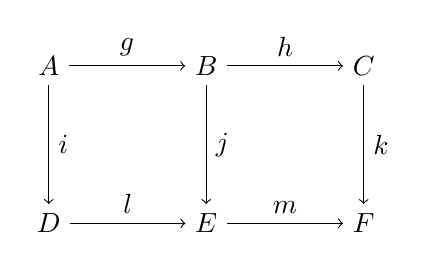
\begin{tikzpicture}[auto]
			\node (a) at (0, 0) {$A$};
			\node (b) at (2, 0) {$B$};
			\node (c) at (4, 0) {$C$};
			\node (d) at (0, -2) {$D$};
			\node (e) at (2, -2) {$E$};
			\node (f) at (4, -2) {$F$};
			\draw[->] (a) to node {$g$}(b);
			\draw[->] (b) to node {$h$}(c);
			\draw[->] (a) to node {$i$}(d);
			\draw[->] (b) to node {$j$}(e);
			\draw[->] (c) to node {$k$}(f);
			\draw[->] (d) to node {$l$}(e);
			\draw[->] (e) to node {$m$}(f);
		\end{tikzpicture}
	\end{center}

	\subsection{元}
		集合の圏では集合から集合への関数の性質を述べるのに集合の元を用いることができるが、圏の対象では一般的に元を取ることができない。
		しかしある圏$\cat{C}$に終対象$1$と呼ばれる特別な対象が存在するとき、$\cat{C}$の任意の対象$A$のある元(global elements)はある射$\mor{a}{1}{A}$で表せる。
		\begin{center}
			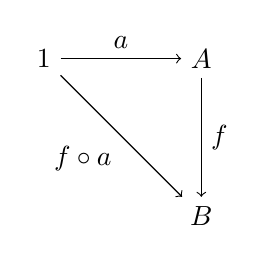
\begin{tikzpicture}[auto]
				\node (a) at (2, 0) {$A$};
				\node (b) at (2, -2) {$B$};
				\node (1) at (0, 0) {$1$};
				\draw[->] (1) to node {$a$}(a);
				\draw[->] (1) to node[swap] {$f\circ a$}(b);
				\draw[->] (a) to node {$f$}(b);
			\end{tikzpicture}
		\end{center}

		射$\mor{f}{A}{B}$に対して$\mor{a}{1}{A}$を適用する操作は、そのまま関数の合成$\mor{f\circ a}{1}{B}$で表せる。
		また射を適用した元もまた終対象からの射になるから$f\circ a$もまた対象$B$の元になる。

		後に詳しく説明するが、要素をただ一つ持つような集合は集合の圏における終対象$1$であり、$1$から集合$A$への写像である元は実際に集合$A$の元とみなせる。
		\begin{prop}[集合の圏における元]
			集合の圏には終対象となる集合$1$が存在し、任意の集合$A$において元$\mor{a}{1}{A}$は集合における元に対し一意に対応する。
		\end{prop}
	\subsection{同型}
	圏論では射の等しさを表すときには等号を使うが、対象に対しての等号は制約が多い。そのため同型と呼ばれる同値関係を代わりに用いる。
	\begin{define}[同型]
		ある対象$A$と$B$が同型、つまり$A\cong B$であるとは、$f\circ f^{-1}=id_B$と$f^{-1}\circ f=id_A$を満たすようなある二つの射$\mor{f}{A}{B}$とその逆射$\mor{f^{-1}}{B}{A}$が存在するときである。
		また、このような射$f,f^{-1}$を同型射と呼ぶ。
	\end{define}
	\begin{center}
		\begin{tikzpicture}[auto]
			\node (a) at (-4, -1) {$A$};
			\node (b) at (-2, -1) {$B$};
			\draw[->,transform canvas={yshift=-3pt}] (a) to node[swap] {$f$}(b);
			\draw[->,transform canvas={yshift=3pt}] (b) to node[swap] {$f^{-1}$}(a);

			\node (a) at (0, 0) {$A$};
			\node (b) at (2, 0) {$B$};
			\node (b') at (0, -2) {$B$};
			\draw[->] (a) to node[swap] {$f$}(b');
			\draw[->] (b) to node {$id_B$}(b');
			\draw[->] (b) to node[swap] {$f^{-1}$}(a);

			\node (a) at (4, 0) {$B$};
			\node (b) at (6, 0) {$A$};
			\node (b') at (4, -2) {$A$};
			\draw[->] (a) to node[swap] {$f^{-1}$}(b');
			\draw[->] (b) to node {$id_A$}(b');
			\draw[->] (b) to node[swap] {$f$}(a);
		\end{tikzpicture}
	\end{center}
	同型は対象同士の相互互換のような関係性を表していると感じられる。
	\begin{prop}[集合の圏の同型]
		$A\cong B$$\Longleftrightarrow$同型射$\mor{i}{A}{B}$が全単射。

		また全単射は、任意の元$\mor{b}{1}{B}$に対して、$i(a)=b$が成り立つようなある元$\mor{a}{1}{A}$が一意に存在することであり、この対応を一対一対応と呼ぶ。
	\end{prop}

	\begin{proof}
		$(\Longleftarrow)$だけ証明する。


		まずは$b$に対する等式を満たすような$a$が存在することを示す
		任意の元$\mor{b}{1}{B}$にたいして対応する元$\mor{a}{1}{A}$を$a=i^{-1}(b)$とする。すると
		\begin{align*}
			i(a)&=i(i^{-1}(b))&\text{(元$a$の定義)}\\
			&=(i\circ i^{-1})(b)&\text{(写像の合成の定義)}\\
			&=b&\text{(同型射の定義)}\\
		\end{align*}
		\[i(a)=i(i^{-1}(b))=i\circ i^{-1}(b)=b\]となり、確かにこのような$a$は存在する。

		$b$に対する元$a$の一意性を示すには、任意の元$\mor{a'}{1}{A}$において$i(a)=b,\ i(a')=b$ならば$a=a'$を示せばよい。

		$i(a')=b$と仮定すると、
		\begin{align*}
			a&=i^{-1}(b)&\text{(元$a$の定義)}\\
			 &=i^{-1}(i(a'))&\text{(仮定)}\\
			 &=(i^{-1}\circ i)(a')&\text{(写像の合成の定義)}\\
			 &=a'&\text{(同型射の定義)}
		\end{align*}
		よって$b$に対する$i(a)=b$を満たすような$a$が一意に存在することが示せたので、$i$が全単射であることが示せた。
	\end{proof}
	\section{普遍性}
	普遍性はある対象と射を特徴づけるために使用され、ある図式を可換にするような射が一意に存在する。というように記述され、図式中の射と一意に定まる射の対応関係を示すことが多い。このような議論は集合の圏における同型でも扱ったが、実際に以下で紹介する普遍性は集合の全単射で表せる。詳しくは別の章で説明する。
	\subsection{積}
	\begin{define}[積]
		対象$A$と$B$が積を持つとは、以下の条件を満たす組$(A\times B,\pi_{L,A},\pi_{R,B})$が存在するときである。
		\begin{quote}
			\begin{description}
			\item[積対象と射影射]ある積対象$A\times B$とある二つの射$\mor{\pi_{L,A}}{A\times B}{A}$、$\mor{\pi_{R,B}}{A\times B}{B}$が存在する。
			この時、積対象と射影射の組$(A\times B,\pi_{L,A},\pi_{R,B})$を$A,B$の積と呼ぶ。


			\begin{center}
				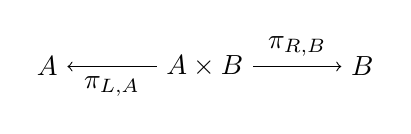
\begin{tikzpicture}[auto]
					\node (a) at (0, 0) {$A$};
					\node (b) at (4, 0) {$B$};
					\node (ab) at (2, 0) {$A\times B$};
					\draw[->] (ab) to node {$\pi_{L,A}$}(a);
					\draw[->] (ab) to node {$\pi_{R,B}$}(b);
				\end{tikzpicture}
			\end{center}
			また$(A\times A,\pi_{L,A},\pi_{R,A})$などの紛らわしい場合を除いて$\pi_{L,A}$を$\pi_A$、$\pi_{R,B}$を$\pi_B$と表記する。
			\item[任意の対象からの射]任意の対象$X$に対し任意の二射$\mor{f}{X}{A}$、$\mor{g}{X}{B}$が存在するとする。
			\begin{center}
				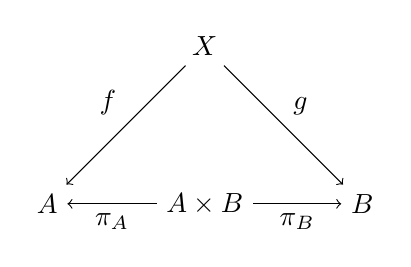
\begin{tikzpicture}[auto]
					\node (a) at (0, 0) {$A$};
					\node (b) at (4, 0) {$B$};
					\node (ab) at (2, 0) {$A\times B$};
					\node (x) at (2, 2) {$X$};
					\draw[->] (ab) to node {$\pi_A$}(a);
					\draw[->] (ab) to node[swap] {$\pi_B$}(b);
					\draw[->] (x) to node[swap] {$f$}(a);
					\draw[->] (x) to node {$g$}(b);
				\end{tikzpicture}
			\end{center}
			\item[普遍性]任意の二射$f,g$に対して図式を可換にする、つまり$\pi_A\circ\tuple{f,g}=f$、$\pi_B\circ\tuple{f,g}=g$が成り立つような射$\tuple{f,g}$を射の対とする。

			またこのような射の対$\tuple{f,g}$は任意の二射$f,g$に対して一意に存在する。

			射の対は一意に存在するが、ある射$h$が二射$f,g$に対する射の対である条件に一意性と存在性は含まれない。射の対であることを示すには単に二つの等式$\pi_A\circ h=f$、$\pi_B\circ h=g$が成り立つことを確認するだけでよい。

			\begin{center}
				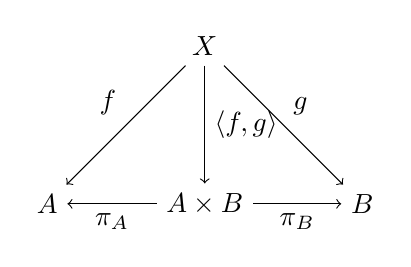
\begin{tikzpicture}[auto]
					\node (a) at (0, 0) {$A$};
					\node (b) at (4, 0) {$B$};
					\node (ab) at (2, 0) {$A\times B$};
					\node (x) at (2, 2) {$X$};
					\draw[->] (ab) to node {$\pi_A$}(a);
					\draw[->] (ab) to node[swap] {$\pi_B$}(b);
					\draw[->] (x) to node[swap] {$f$}(a);
					\draw[->] (x) to node {$g$}(b);
					\draw[->] (x) to node {$\tuple{f,g}$}(ab);
				\end{tikzpicture}
			\end{center}
			\end{description}
		\end{quote}

	\end{define}

	射の対が一意であるとは、射の対$\tuple{f,g}$に対し、ある射$\mor{h}{X}{A\times B}$が存在して$\pi_A\circ h=f$、$\pi_B\circ h=g$を満たすとき、$h=\tuple{f,g}$となることである。


	また、図式を可換にする射の対$\tuple{f,g}$の存在性は任意の射の組み合わせに対して射の対が存在することを示し、一意性は射の対が含んでいる二つの射以外の判別可能な要素を含みようがないことを示している。

	\begin{define}[積を持つ圏]
		すべての圏、すべての二対象に対して積が存在するとは限らないが、ある圏$\cat{C}$の任意の二対象に対して積が存在するとき、圏$\cat{C}$は積を持つという。
	\end{define}
	ここで$X$に終対象$1$を当てはめると、元$\mor{a}{1}{A}$、元$\mor{b}{1}{B}$に対して$\pi_A\circ\tuple{a,b}=a$、$\pi_B\circ\tuple{a,b}=b$が成り立つような$\tuple{a,b}$が一意に存在することがわかる。
	\begin{center}
		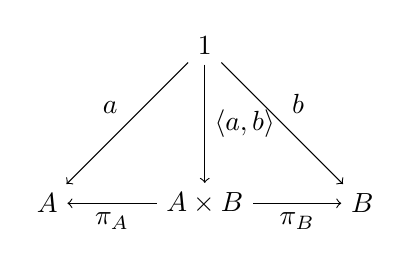
\begin{tikzpicture}[auto]
			\node (a) at (0, 0) {$A$};
			\node (b) at (4, 0) {$B$};
			\node (ab) at (2, 0) {$A\times B$};
			\node (x) at (2, 2) {$1$};
			\draw[->] (ab) to node {$\pi_A$}(a);
			\draw[->] (ab) to node[swap] {$\pi_B$}(b);
			\draw[->] (x) to node[swap] {$a$}(a);
			\draw[->] (x) to node {$b$}(b);
			\draw[->] (x) to node {$\tuple{a,b}$}(ab);
		\end{tikzpicture}
	\end{center}

	次に積の性質をいくつか見ていく。
	\begin{prop}[射の対の分配則]
		$\mor{f}{X}{A}$、$\mor{g}{X}{B}$、$\mor{h}{Y}{X}$に対して\[\tuple{f,g}\circ h=\tuple{f\circ h,g\circ h}\]が成り立つ
	\end{prop}
	\begin{proof}
		積$A\times B$に対し、$\mor{f\circ h}{Y}{A}$、$\mor{g\circ h}{Y}{B}$の射の対$\mor{\tuple{f\circ h,g\circ h}}{Y}{A\times B}$を考える。

		これは$\mor{\tuple{f,g}\circ h}{Y}{A\times B}$が二射$f\circ h,g\circ h$における射の対となることを示し、射の対の一意性から証明すればよい。

		積の普遍性より、
		\begin{align*}
			\pi_A\circ\tuple{f\circ h,g\circ h}&=f\circ h\\
			\pi_B\circ\tuple{f\circ h,g\circ h}&=g\circ h
		\end{align*}
		が成り立つような射$\tuple{f\circ h,g\circ h}$は一意に存在する。

		また、
		\begin{align*}
			\pi_A\circ(\tuple{f,g}\circ h)&=(\pi_A\circ\tuple{f,g})\circ h&\text{(結合則)}\\
			&=f\circ h&\text{(射の対の可換性)}\\
			\pi_B\circ(\tuple{f,g}\circ h)&=(\pi_B\circ\tuple{f,g})\circ h&\text{(結合則)}\\
			&=g\circ h&\text{(射の対の可換性)}
		\end{align*}
		$\pi_A\circ(\tuple{f,g}\circ h)=f\circ h$、$\pi_B\circ(\tuple{f,g}\circ h)=g\circ h$となるため、$\mor{\tuple{f,g}\circ h}{Y}{A\times B}$も同様に二射$f\circ h,g\circ h$の射の対になる。
		よって射の対の一意性より、$\tuple{f,g}\circ h=\tuple{f\circ h,g\circ h}$が成り立つ。
	\end{proof}

	\begin{center}
		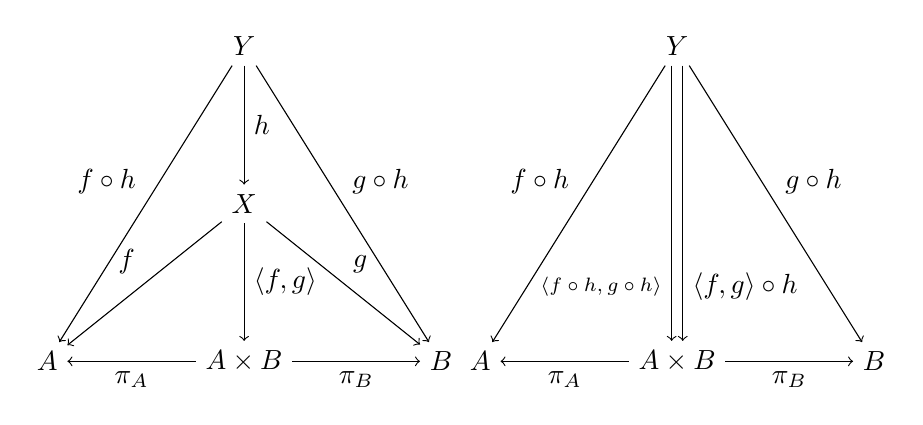
\begin{tikzpicture}[auto]
			\node (y) at (3, 4) {$Y$};
			\node (a) at (0.5, 0) {$A$};
			\node (b) at (5.5, 0) {$B$};
			\node (ab) at (3, 0) {$A\times B$};
			\node (x) at (3, 2) {$X$};
			\draw[->] (y) to node {$h$}(x);
			\draw[->] (y) to node[swap] {$f\circ h$}(a);
			\draw[->] (y) to node {$g\circ h$}(b);
			\draw[->] (ab) to node {$\pi_A$}(a);
			\draw[->] (ab) to node[swap] {$\pi_B$}(b);
			\draw[->] (x) to node[swap] {$f$}(a);
			\draw[->] (x) to node {$g$}(b);
			\draw[->] (x) to node {$\tuple{f,g}$}(ab);

			\node (y) at (8.5, 4) {$Y$};
			\node (a) at (6, 0) {$A$};
			\node (b) at (11, 0) {$B$};
			\node (ab) at (8.5, 0) {$A\times B$};
			\draw[->, transform canvas={xshift=2pt}] (y) to node[yshift=-30pt] {$\tuple{f,g}\circ h$}(ab);
			\draw[->, transform canvas={xshift=-2pt}] (y) to node[yshift=-30pt, swap] {\scriptsize{$\tuple{f\circ h,g\circ h}$}}(ab);
			\draw[->] (y) to node[swap] {$f\circ h$}(a);
			\draw[->] (y) to node {$g\circ h$}(b);
			\draw[->] (ab) to node {$\pi_A$}(a);
			\draw[->] (ab) to node[swap] {$\pi_B$}(b);
		\end{tikzpicture}
	\end{center}
	また$Y$に終対象$1$、$h$に元$\mor{x}{1}{X}$を当てはめると、同様に$\tuple{f,g}\circ x=\tuple{f\circ x,g\circ x}$となる。
	つまり射の対は与えられた元にそれぞれの射を適用し、また対を取るような射だと考えられる。
	\begin{center}
		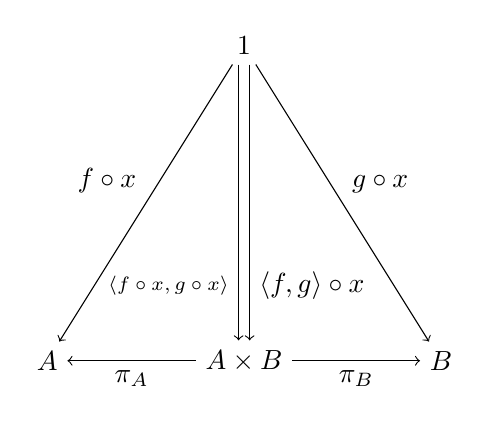
\begin{tikzpicture}[auto]
			\node (y) at (8.5, 4) {$1$};
			\node (a) at (6, 0) {$A$};
			\node (b) at (11, 0) {$B$};
			\node (ab) at (8.5, 0) {$A\times B$};
			\draw[->, transform canvas={xshift=2pt}] (y) to node[yshift=-30pt] {$\tuple{f,g}\circ x$}(ab);
			\draw[->, transform canvas={xshift=-2pt}] (y) to node[yshift=-30pt, swap] {\scriptsize{$\tuple{f\circ x,g\circ x}$}}(ab);
			\draw[->] (y) to node[swap] {$f\circ x$}(a);
			\draw[->] (y) to node {$g\circ x$}(b);
			\draw[->] (ab) to node {$\pi_A$}(a);
			\draw[->] (ab) to node[swap] {$\pi_B$}(b);
		\end{tikzpicture}
	\end{center}

	次に、任意の積から任意の積への射である、射の積を定義していく。
	\begin{define}[射の積]
		射$\mor{f}{A}{A'}$、$\mor{g}{B}{B'}$に対して射の積$\mor{f\times g}{A\times B}{A'\times B'}$を\[f\times g = \tuple{f\circ\pi_A,g\circ\pi_B}\]と定義する。
		\begin{center}
			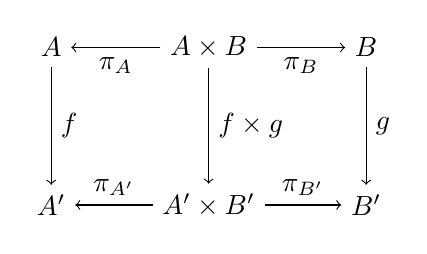
\begin{tikzpicture}[auto]
				\node (a) at (0, 0) {$A$};
				\node (ab) at (2, 0) {$A\times B$};
				\node (b) at (4, 0) {$B$};
				\node (a') at (0, -2) {$A'$};
				\node (a'b') at (2, -2) {$A'\times B'$};
				\node (b') at (4, -2) {$B'$};
				\draw[->] (a'b') to node[swap] {$\pi_{A'}$}(a');
				\draw[->] (a'b') to node {$\pi_{B'}$}(b');
				\draw[->] (ab) to node {$\pi_A$}(a);
				\draw[->] (ab) to node[swap] {$\pi_B$}(b);
				\draw[->] (a) to node {$f$}(a');
				\draw[->] (b) to node {$g$}(b');
				\draw[->] (ab) to node {$f\times g$}(a'b');
			\end{tikzpicture}
		\end{center}
	\end{define}
	射の対は任意の対象から任意の積への射であるのに対し、射の積は任意の積から任意の積への射である。
	二つの対象から二つの対象へ射を一つの射に纏めることから、直感的に射の積は並列処理のように思える。

	\begin{prop}[積と合成の交換]
		射の積$\mor{f\times g}{A\times B}{A'\times B'}$、$\mor{f'\times g'}{A'\times B'}{A''\times B''}$に対して、\[(f'\times g')\circ(f\times g)=(f'\circ f)\times(g'\circ g)\]が成り立つ。
	\end{prop}
	\begin{proof}
		積$(A''\times B'',\pi_{A''},\pi_{B''})$において対$(X,f,g)$に$(A\times B,f'\circ f\circ\pi_A$,$g'\circ g\circ\pi_B)$を当てはめると射$\mor{\tuple{f'\circ f\circ\pi_A,g'\circ g\circ\pi_B}}{A\times B}{A''\times B''}$が得られる。また射の積の定義より\[\tuple{f'\circ f\circ\pi_A,g'\circ g\circ\pi_B}=(f'\circ f)\times(g'\circ g)\]が成り立つ。
		次に$(f'\times g')\circ(f\times g)$も同様に$(A\times B,f'\circ f\circ\pi_A$,$g'\circ g\circ\pi_B)$に対する射の対であることを示す。
		\begin{align*}
			\pi_{A''}\circ(f'\times g')\circ(f\times g)&=\pi_{A''}\circ\tuple{f'\circ\pi_A,g'\circ\pi_B}\circ\tuple{f\circ\pi_A,g\circ\pi_B}&\text{(射の積の定義)}\\
			&=f'\circ\pi_{A'}\circ\tuple{f\circ\pi_A,g\circ\pi_B}&\text{(射の対の可換性)}\\
			&=f'\circ f\circ\pi_A&\text{(射の対の可換性)}\\
			\pi_B\circ(f'\times g')\circ(f\times g)&=\pi_{B''}\circ\tuple{f'\circ\pi_A,g'\circ\pi_B}\circ\tuple{f\circ\pi_A,g\circ\pi_B}&\text{(射の積の定義)}\\
			&=g'\circ\pi_{B'}\circ\tuple{f\circ\pi_A,g\circ\pi_B}&\text{(射の対の可換性)}\\
			&=g'\circ g\circ\pi_B&\text{(射の対の可換性)}
		\end{align*}
	\begin{center}
		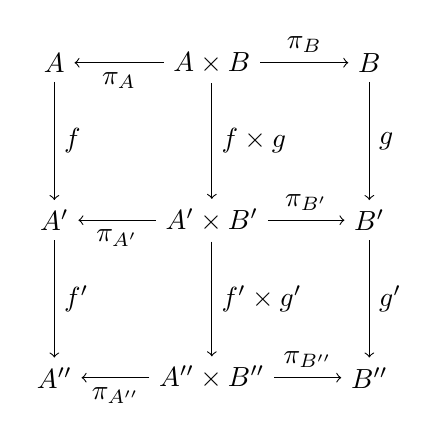
\begin{tikzpicture}[auto]
			\node (a) at (0, 0) {$A$};
			\node (a') at (0, -2) {$A'$};
			\node (a'') at (0, -4) {$A''$};
			\node (ab) at (2, 0) {$A\times B$};
			\node (ab') at (2, -2) {$A'\times B'$};
			\node (ab'') at (2, -4) {$A''\times B''$};
			\node (b) at (4, 0) {$B$};
			\node (b') at (4, -2) {$B'$};
			\node (b'') at (4, -4) {$B''$};
			\draw[->] (ab) to node{$\pi_{A}$}(a);
			\draw[->] (ab) to node{$\pi_{B}$}(b);
			\draw[->] (ab') to node{$\pi_{A'}$}(a');
			\draw[->] (ab') to node{$\pi_{B'}$}(b');
			\draw[->] (ab'') to node{$\pi_{A''}$}(a'');
			\draw[->] (ab'') to node{$\pi_{B''}$}(b'');
			\draw[->] (a) to node{$f$}(a');
			\draw[->] (a') to node{$f'$}(a'');
			\draw[->] (b) to node{$g$}(b');
			\draw[->] (b') to node{$g'$}(b'');
			\draw[->] (ab) to node{$f\times g$}(ab');
			\draw[->] (ab') to node{$f'\times g'$}(ab'');
		\end{tikzpicture}
		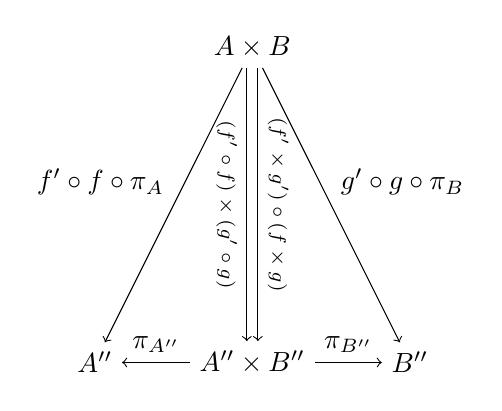
\begin{tikzpicture}[auto]
			\node (a'') at (0, -4) {$A''$};
			\node (ab) at (2, 0) {$A\times B$};
			\node (ab'') at (2, -4) {$A''\times B''$};
			\node (b'') at (4, -4) {$B''$};
			\draw[->] (ab) to node[swap]{$f'\circ f\circ\pi_A$}(a'');
			\draw[->] (ab) to node{$g'\circ g\circ\pi_B$}(b'');
			\draw[->] (ab'') to node[swap]{$\pi_{A''}$}(a'');
			\draw[->] (ab'') to node{$\pi_{B''}$}(b'');
			\draw[->,transform canvas={xshift=2pt}] (ab) to node[sloped]{\scriptsize{$(f'\times g')\circ(f\times g)$}} (ab'');
			\draw[->,transform canvas={xshift=-2pt}] (ab) to node[sloped,swap]{\scriptsize{$(f'\circ f)\times(g'\circ g)$}}(ab'');
		\end{tikzpicture}
	\end{center}

		\[\pi_A\circ(f'\times g')\circ(f\times g)=f'\circ f\circ\pi_A,\ \pi_B\circ(f'\times g')\circ(f\times g)=g'\circ g\circ\pi_B\]の二式が成り立つから、$(f'\times g')\circ(f\times g)$も同様に$(A\times B,f'\circ f\circ\pi_A$,$g'\circ g\circ\pi_B)$に対する射の対である。

		よって$(f'\times g')\circ(f\times g)=(f'\circ f)\times(g'\circ g)$が成り立つ。
	\end{proof}
	射の積を並列での合成とみなすならば、射の合成は直列での合成を表し、積と合成の交換はどちらの合成を先に計算しても結果が変わらないことを表す。
	\begin{prop}[射影射の対]
		ある積$(A\times B,\pi_A,\pi_B)$に対して$\tuple{\pi_A,\pi_B}=id_{A\times B}$が成り立つ。
	\end{prop}
	\begin{proof}
		積$(A\times B,\pi_A,\pi_B)$に対して二射$\pi_A,\pi_B$の射の対$\mor{\tuple{\pi_A,\pi_B}}{A\times B}{A\times B}$を考える。この時、$\mor{id_{A\times B}}{A\times B}{A\times B}$も同様に二射$\pi_A,\pi_B$の射の対であることを示せばよい。


		$\pi_{A}\circ id_{A\times B}=\pi_{A}$と$\pi_{B}\circ id_{A\times B}=\pi_{B}$が成り立つから、$id_{A\times B}$は$\pi_A$と$\pi_B$の射の対になる。よって射の対の一意性より、$\tuple{\pi_A,\pi_B}=id_{A\times B}$が成り立つ。
		\begin{center}
			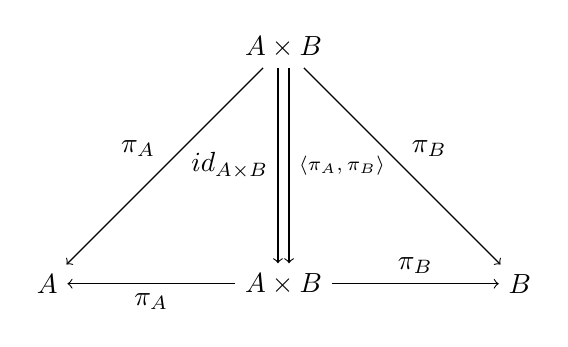
\begin{tikzpicture}[auto]
				\node (a) at (0, 0) {$A$};
				\node (ab) at (3, 0) {$A\times B$};
				\node (b) at (6, 0) {$B$};
				\node (p) at (3, 3) {$A\times B$};
				\draw[->] (p) to node[swap]{$\pi_A$}(a);
				\draw[->] (p) to node{$\pi_B$}(b);
				\draw[->,transform canvas={xshift=2pt}] (p) to node{\scriptsize{$\tuple{\pi_A,\pi_B}$}}(ab);
				\draw[->,transform canvas={xshift=-2pt}] (p) to node[swap]{$id_{A\times B}$}(ab);
				\draw[->] (ab) to node{$\pi_A$}(a);
				\draw[->] (ab) to node{$\pi_B$}(b);
			\end{tikzpicture}
		\end{center}
	\end{proof}
	\begin{prop}[積の一意性]
		$A$と$B$の積$A\times B$に対して、同様に$A$と$B$の積である対象$P$と射影射$\mor{\rho_A}{P}{A}$、$\mor{\rho_B}{P}{B}$が存在するとき、$A\times B\cong P$が成り立つ。またこの時、積は同型を除いて一意と呼ぶことがある。
	\end{prop}
	\begin{proof}
		対象$A$、$B$の積$(A\times B,\pi_A,\pi_B)$、$(P,\rho_A,\rho_B)$の二つの積を考える必要があるが、ややこしいので少し性質を整理する。
		\begin{quote}
			\begin{description}
				\item[積$(A\times B,\pi_A,\pi_B)$の性質]
				積$A\times B$と射影射$\mor{\pi_A}{A\times B}{A}$、$\mor{\pi_B}{A\times B}{B}$において二つの射$\mor{f}{X}{A}$、$\mor{g}{X}{B}$に対する射の対を$\mor{\tuple{f,g}}{X}{A\times B}$とする。また射$\tuple{f,g}$が積$A\times B$における射の対であるとき、
				\begin{align*}
					\pi_A\circ\tuple{f,g}&=f\\
					\pi_B\circ\tuple{f,g}&=g
				\end{align*}
				が成り立つ。
				またこのような射の対は一意に存在する。
				\begin{center}
					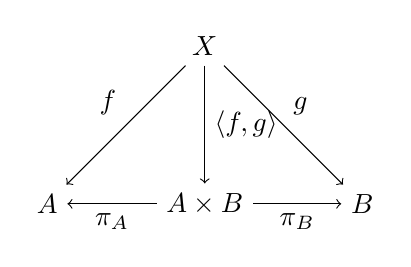
\begin{tikzpicture}[auto]
						\node (a) at (0, 0) {$A$};
						\node (b) at (4, 0) {$B$};
						\node (ab) at (2, 0) {$A\times B$};
						\node (x) at (2, 2) {$X$};
						\draw[->] (ab) to node {$\pi_A$}(a);
						\draw[->] (ab) to node[swap] {$\pi_B$}(b);
						\draw[->] (x) to node[swap] {$f$}(a);
						\draw[->] (x) to node {$g$}(b);
						\draw[->] (x) to node {$\tuple{f,g}$}(ab);
					\end{tikzpicture}
				\end{center}
				\item[積$(P,\rho_A,\rho_B)$の性質]
				積$P$と射影射$\mor{\rho_A}{P}{A}$、$\mor{\rho_B}{P}{B}$において二つの射$\mor{f}{X}{A}$、$\mor{g}{X}{B}$に対する射の対を$\mor{[f,g]}{X}{P}$とする。また射$[f,g]$が積$P$における射の対であるとき、
				\begin{align*}
					\rho_A\circ[f,g]&=f\\
					\rho_B\circ[f,g]&=g
				\end{align*}
				が成り立つ。
				またこのような射の対は一意に存在する。
				\begin{center}
					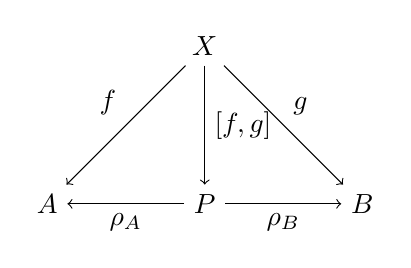
\begin{tikzpicture}[auto]
						\node (a) at (0, 0) {$A$};
						\node (b) at (4, 0) {$B$};
						\node (ab) at (2, 0) {$P$};
						\node (x) at (2, 2) {$X$};
						\draw[->] (ab) to node {$\rho_A$}(a);
						\draw[->] (ab) to node[swap] {$\rho_B$}(b);
						\draw[->] (x) to node[swap] {$f$}(a);
						\draw[->] (x) to node {$g$}(b);
						\draw[->] (x) to node {$[f,g]$}(ab);
					\end{tikzpicture}
				\end{center}
			\end{description}

			積$A\times B$における射の対$\mor{\tuple{f,g}}{X}{A\times B}$に対し、積$P$における射の対$\mor{[f,g]}{X}{P}$は全く別の射である。そのため対の表記で区別することにする。

			また$\pi_A\circ[f,g]=f$は成り立たないどころか、ドメイン、コドメインは$\mor{\pi_A}{A\times B}{A}$と$\mor{[f,g]}{X}{P}$となり合成すらできないということに注意してほしい。
		\end{quote}
		証明に戻ると、\[[\pi_A,\pi_B]\circ\tuple{\rho_A,\rho_B}=id_P\]と
		\[\tuple{\rho_A,\rho_B}\circ[\pi_A,\pi_B]=id_{A\times B}\]が成り立つことを二つの積の普遍性による射の一意性から示せばよい。

		積$(A\times B,\pi_A,\pi_B)$において、二射$\rho_A,\rho_B$に対する射の対を\[\mor{\tuple{\rho_A,\rho_B}}{P}{A\times B}\]とする。

		逆に積$(P,\rho_A,\rho_B)$において二射$\pi_A,\pi_B$に対する射の対を\[\mor{[\pi_A,\pi_B]}{A\times B}{P}\]とする。
		\begin{center}
			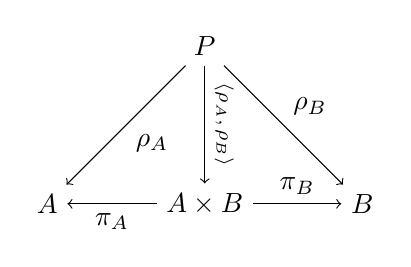
\begin{tikzpicture}[auto]
				\node (a) at (0, 0) {$A$};
				\node (ab) at (2, 0) {$A\times B$};
				\node (b) at (4, 0) {$B$};
				\node (p) at (2, 2) {$P$};
				\draw[->] (p) to node{$\rho_A$}(a);
				\draw[->] (p) to node{$\rho_B$}(b);
				\draw[->] (p) to node[sloped]{\scriptsize{$\tuple{\rho_A,\rho_B}$}}(ab);
				\draw[->] (ab) to node{$\pi_A$}(a);
				\draw[->] (ab) to node{$\pi_B$}(b);
			\end{tikzpicture}
			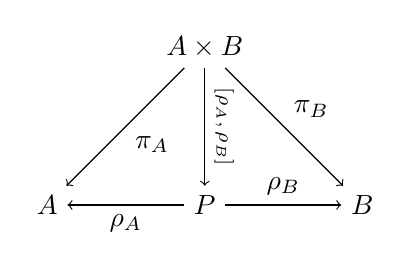
\begin{tikzpicture}[auto]
				\node (a) at (0, 0) {$A$};
				\node (ab) at (2, 2) {$A\times B$};
				\node (b) at (4, 0) {$B$};
				\node (p) at (2, 0) {$P$};
				\draw[->] (p) to node{$\rho_A$}(a);
				\draw[->] (p) to node{$\rho_B$}(b);
				\draw[->] (ab) to node[sloped]{\scriptsize{$[\rho_A,\rho_B]$}}(p);
				\draw[->] (ab) to node{$\pi_A$}(a);
				\draw[->] (ab) to node{$\pi_B$}(b);
			\end{tikzpicture}
		\end{center}
		次に$\mor{\tuple{\rho_A,\rho_B}\circ[\pi_A,\pi_B]}{A\times B}{A\times B}$が$\pi_A$と$\pi_B$の射の対であることを示す。
		\begin{align*}
			\pi_A\circ\tuple{\rho_A,\rho_B}\circ[\pi_A,\pi_B]&=\rho_A\circ[\pi_A,\pi_B]&\text{(積$A\times B$の射の対の可換性)}\\
			&=\pi_A&\text{(積$P$の射の対の可換性)}\\
			\pi_B\circ\tuple{\rho_A,\rho_B}\circ[\pi_A,\pi_B]&=\rho_B\circ[\pi_A,\pi_B]&\text{(積$A\times B$の射の対の可換性)}\\
			&=\pi_B&\text{(積$P$の射の対の可換性)}\\
		\end{align*}
		よって\[\pi_A\circ(\tuple{\rho_A,\rho_B}\circ[\pi_A,\pi_B])=\pi_A,\ \pi_B\circ(\tuple{\rho_A,\rho_B}\circ[\pi_A,\pi_B])=\pi_B\]が成り立つから、$\tuple{\rho_A,\rho_B}\circ[\pi_A,\pi_B]$は射$\pi_A$と$\pi_B$の射の対となる。すると射の対の一意性より、\[\tuple{\rho_A,\rho_B}\circ[\pi_A,\pi_B]=\tuple{\pi_A,\pi_B}=id_{A\times B}\]が成り立つ。
		\begin{center}
			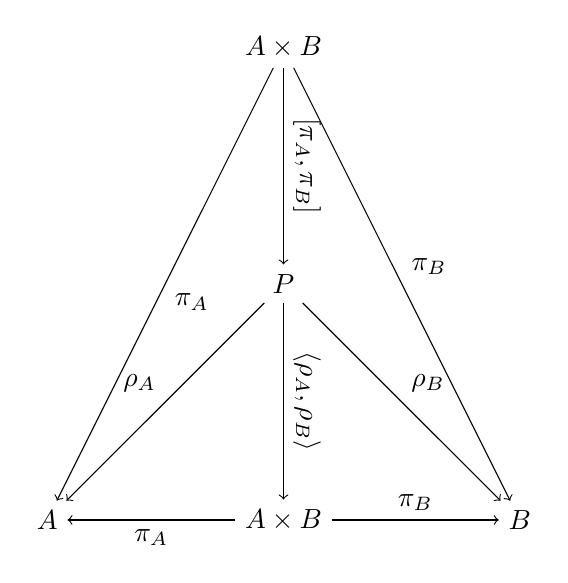
\begin{tikzpicture}[auto]
				\node (a) at (0, 0) {$A$};
				\node (ab) at (3, 0) {$A\times B$};
				\node (ab2) at (3, 6) {$A\times B$};
				\node (b) at (6, 0) {$B$};
				\node (p) at (3, 3) {$P$};
				\draw[->] (p) to node[swap]{$\rho_A$}(a);
				\draw[->] (p) to node{$\rho_B$}(b);
				\draw[->] (p) to node[sloped]{$\tuple{\rho_A,\rho_B}$}(ab);
				\draw[->] (ab2) to node[sloped]{$[\pi_A,\pi_B]$}(p);
				\draw[->] (ab) to node{$\pi_A$}(a);
				\draw[->] (ab) to node{$\pi_B$}(b);
				\draw[->] (ab2) to node{$\pi_A$}(a);
				\draw[->] (ab2) to node{$\pi_B$}(b);
			\end{tikzpicture}
			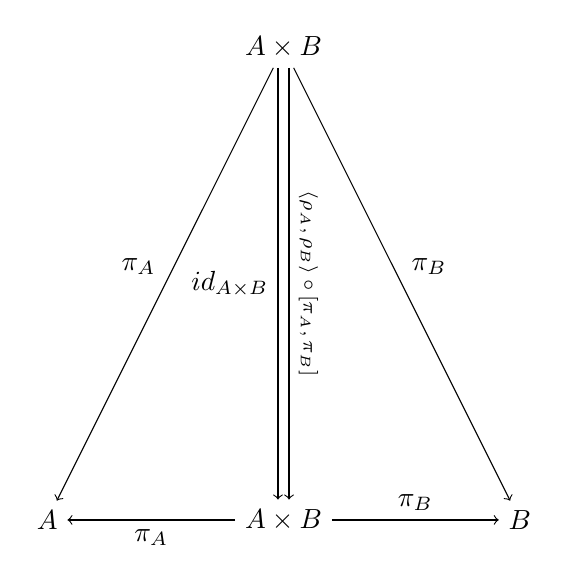
\begin{tikzpicture}[auto]
				\node (a) at (0, 0) {$A$};
				\node (ab) at (3, 0) {$A\times B$};
				\node (b) at (6, 0) {$B$};
				\node (ab2) at (3, 6) {$A\times B$};
				\draw[->] (ab2) to node[swap]{$\pi_A$}(a);
				\draw[->] (ab2) to node{$\pi_B$}(b);
				\draw[->,transform canvas={xshift=2pt}] (ab2) to node[sloped]{\scriptsize{$\tuple{\rho_A,\rho_B}\circ[\pi_A,\pi_B]$}}(ab);
				\draw[->,transform canvas={xshift=-2pt}] (ab2) to node[swap]{$id_{A\times B}$}(ab);
				\draw[->] (ab) to node{$\pi_A$}(a);
				\draw[->] (ab) to node{$\pi_B$}(b);
			\end{tikzpicture}
		\end{center}
		同様に$[\pi_A,\pi_B]\circ\tuple{\rho_A,\rho_B}=id_P$が成り立つから、$[\pi_A,\pi_B]$と$\tuple{\rho_A,\rho_B}$は同型射となり、$A\times B\cong P$が成り立つ。
	\end{proof}
	\subsection{集合の圏と積}
	次に集合の圏$\cat{Set}$と積の関係性を示す。元を指定して直接直積集合を定義する方法と、普遍性を用いて直積集合の周りの写像の性質を述べて定義する方法の二つが同値であることを確認してほしい。
	\begin{define}[直積集合]
		集合$A$と$B$の直積集合$A\times B$を\[A\times B =\{\tuple{a,b}\ |\ a\in A,\ b\in B\}\]と定義する。
	\end{define}
	\begin{prop}
		集合の圏$\cat{Set}$の対象$A$と$B$の積$A\times B$は集合$A$と$B$の直積集合である。
	\end{prop}
	\begin{proof}
		任意の元$\mor{a}{1}{A}$、$\mor{b}{1}{B}$に対して射の対の存在性により元の対$\mor{\tuple{a,b}}{1}{A\times B}$が存在する。
		また、$A\times B$の任意の元$\mor{f}{1}{A\times B}$は射影射との合成\[\pi_A\circ f=a',\ \pi_B\circ f=b'\]により、何かしらの元$a',b'$に分解できる。この時、射の対の一意性から$f=\tuple{a',b'}$が成り立つから、$f$は元の対であり順序対になる。そのため順序対とならないような元は含まれないことがわかる。

		よって実際に積$A\times B$は集合$A$と$B$の直積集合であることが示せた。
		\begin{center}
			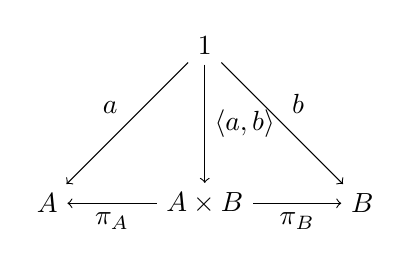
\begin{tikzpicture}[auto]
				\node (a) at (0, 0) {$A$};
				\node (b) at (4, 0) {$B$};
				\node (ab) at (2, 0) {$A\times B$};
				\node (x) at (2, 2) {$1$};
				\draw[->] (ab) to node {$\pi_A$}(a);
				\draw[->] (ab) to node[swap] {$\pi_B$}(b);
				\draw[->] (x) to node[swap] {$a$}(a);
				\draw[->] (x) to node {$b$}(b);
				\draw[->] (x) to node {$\tuple{a,b}$}(ab);
			\end{tikzpicture}
		\end{center}
	\end{proof}

	\begin{prop}
	集合$A$と$B$の直積集合$A\times B$は集合の圏$\cat{Set}$における積である。
	\end{prop}
	\begin{proof}
		限定的ではあるが、まずは任意の対象$X$に終対象$1$を当てはめた場合を見ていき、その後任意の対象$X$に拡張する。
		射影射となる射影写像$\pi_A,\pi_B$を任意の順序対$\tuple{a,b}$において\[\pi_A(\tuple{a,b})=a,\ \pi_B(\tuple{a,b})=b\]と定義する。

		直積集合の定義より、任意の元$a$、$b$に対して順序対$\tuple{a,b}$が存在し、順序対ではない元や重複する元を含まないことから、積の普遍性を部分的に満たすことがわかる。
		\begin{center}
			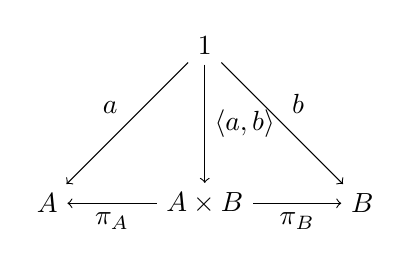
\begin{tikzpicture}[auto]
				\node (a) at (0, 0) {$A$};
				\node (b) at (4, 0) {$B$};
				\node (ab) at (2, 0) {$A\times B$};
				\node (x) at (2, 2) {$1$};
				\draw[->] (ab) to node {$\pi_A$}(a);
				\draw[->] (ab) to node[swap] {$\pi_B$}(b);
				\draw[->] (x) to node[swap] {$a$}(a);
				\draw[->] (x) to node {$b$}(b);
				\draw[->] (x) to node {$\tuple{a,b}$}(ab);
			\end{tikzpicture}
		\end{center}
		次に元の対から写像の対に拡張して考える。写像の対が一意に存在することを元の対が一意に存在することから示せばよい。

		写像$\mor{f}{X}{A}$と写像$\mor{g}{X}{B}$の写像の対$\tuple{f,g}$を$X$の任意の元$x$に対して\[\tuple{f,g}(x)=\tuple{f(x),g(x)}\]と定義する。

		また、
		\begin{align*}
			(\pi_A\circ\tuple{f,g})(x)&=\pi_A(\tuple{f,g}(x))&\text{(写像の合成の定義)}\\
			&=\pi_A(\tuple{f(x),g(x)})&\text{(写像の対の定義)}\\
			&=f(x)&\text{(元の対の可換性)}\\
			(\pi_B\circ\tuple{f,g})(x)&=\pi_B(\tuple{f,g}(x))&\text{(写像の合成の定義)}\\
			&=\pi_B(\tuple{f(x),g(x)})&\text{(写像の対の定義)}\\
			&=g(x)&\text{(元の対の可換性)}
		\end{align*}
		よって\[\pi_A\circ\tuple{f,g}=f,\ \pi_B\circ\tuple{f,g}=g\]が成り立つから写像の対は射の対としての可換性を満たすことがわかる。
		またこのような射の対は$\mor{f}{X}{A}$、$\mor{g}{X}{B}$なる任意の二射$f,g$に対し存在する。

		仮に$\pi_A\circ h=f,\ \pi_B\circ h=g$となる射$\mor{h}{X}{A\times B}$が存在しても、
		$\pi_A(h(x))=f(x),\ \pi_B(h(x))=g(x)$と元の対の一意性より$h(x)=\tuple{f(x),g(x)}$が成り立ち$h=\tuple{f,g}$となる。よって写像$f,g$の写像の対$\tuple{f,g}$は一意に存在する。
		\begin{center}
			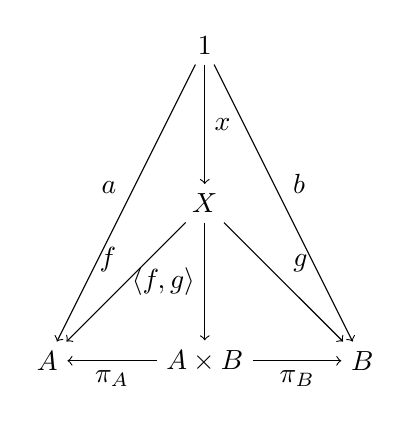
\begin{tikzpicture}[auto]
				\node (a) at (0, 0) {$A$};
				\node (b) at (4, 0) {$B$};
				\node (ab) at (2, 0) {$A\times B$};
				\node (i) at (2, 4) {$1$};
				\node (x) at (2, 2) {$X$};
				\draw[->] (ab) to node {$\pi_A$}(a);
				\draw[->] (ab) to node[swap] {$\pi_B$}(b);
				\draw[->] (x) to node[swap] {$f$}(a);
				\draw[->] (x) to node {$g$}(b);
				\draw[->] (x) to node[swap] {$\tuple{f,g}$}(ab);
				\draw[->] (i) to node[swap] {$a$}(a);
				\draw[->] (i) to node {$b$}(b);
				\draw[->] (i) to node {$x$}(x);
			\end{tikzpicture}
		\end{center}
	\end{proof}

	圏を定義する際に使用した射集合だが、射集合も集合であるため集合の圏の対象として捉えることができる。この射集合が集合の圏の中でどのような性質を持っているのかを直積集合と共に確認していく。
	また射集合は任意の圏に存在するが、今回扱う圏はすべて集合の圏とする。

	\begin{define}[評価射]
		集合の圏$\cat{Set}$の任意の対象$A,B$と$B$の元$b$、$\cat{Set}$の射$\mor{f}{B}{A}$に対して評価射を
		\begin{align*}
			\mor{&ev_{A,B}}{\arset{Set}{B}{A}\times B}{A}\\
			&ev_{A,B}(\tuple{f,b})=f(b)\\
		\end{align*}
		と定義する。これは元$b$に写像$f$を適用する操作を写像にしたものである。
		また厳密な証明は行わないが評価射は実際に写像になる。
	\end{define}
	\begin{define}[余評価射]
		集合の圏$\cat{Set}$の任意の対象$A,B$と$A$の元$a$に対して余評価射を
		\begin{align*}
			\mor{&ce_{A,B}}{A}{\arset{Set}{B}{A\times B}}\\
			&ce_{A,B}(a)=g_a\\
			&g_a(b)=\tuple{a,b}
		\end{align*}
		と定義する。また\[ce_{A,B}(a)(b)=\tuple{a,b}\]とも表記でき、この余評価射も同様に写像になる。
	\end{define}

	この評価射、余評価射は集合の圏の射集合の持つ性質というより、集合の圏の射集合の定義のうちの一つと捉えることができる。
	これらの射の性質を扱うにはまだ道具が足りないため現段階では述べないが、以降から射集合を集合の圏の対象とみなす機会が増えるため、確認も込めてこれらの射を定義した。
	\subsection{終対象}
	\begin{define}[終対象]
		ある圏$\cat{C}$に終対象が存在するとは、ある対象$1$が存在して圏$\cat{C}$の任意の対象$X$に対し射$\mor{!_X}{X}{1}$が一意に存在するときである。

		元を取る操作とは射の向きが逆であることに注意してほしい。
	\end{define}
	射の対$\mor{\tuple{f,g}}{X}{A\times B}$は対象$X$と射$f,g$に対して一意に存在するのであったが、終対象への射$\mor{!_X}{X}{1}$は対応する射が存在しない。そのため、終対象への射は対象$X$に対して無条件で一意に存在することになる。
	\begin{prop}[終対象から終対象への射]
		終対象から終対象への射は恒等射ただ一つである。
	\end{prop}
	\begin{proof}
		終対象$1$に対して、終対象から終対象への射$\mor{!_1}{1}{1}$は無条件で一意に定まる。
		すべての対象に恒等射は存在するから$id_1=!_1$となる。
		\begin{center}
			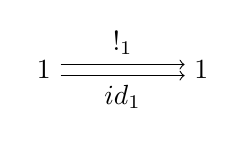
\begin{tikzpicture}[auto]
				\node (1) at (0, 0) {$1$};
				\node (1') at (2, 0) {$1$};
				\draw[->,transform canvas={yshift=2pt}] (1) to node{$!_{1}$}(1');
				\draw[->,transform canvas={yshift=-2pt}] (1) to node[swap]{$id_1$}(1');
			\end{tikzpicture}
		\end{center}
	\end{proof}

	\begin{prop}[終対象の一意性]
		終対象$1$に対して別の終対象$I$が存在するとき、$1\cong I$が成り立つ。
	\end{prop}
	\begin{proof}
		終対象$1$における$I$からの一意に定まる射$\mor{!_I}{I}{1}$と終対象$I$における$1$からの一意に定まる射$\mor{i_1}{1}{I}$の合成$\mor{!_I\circ i_1}{1}{1}$と$\mor{i_1\circ!_I}{I}{I}$はそれぞれ終対象から終対象への射である。

		よって$!_I\circ i_1=id_1$と$i_1\circ!_I=id_I$が成り立ち、$!_I$、$i_1$が同型射になるから$1\cong I$が成り立つ。
		\begin{center}
			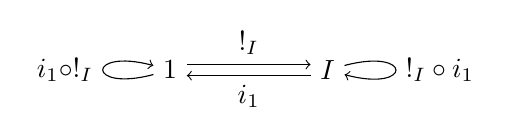
\begin{tikzpicture}[auto]
				\node (1) at (0, 0) {$1$};
				\node (1') at (2, 0) {$I$};
				\draw[->,transform canvas={yshift=2pt}] (1) to node{$!_I$}(1');
				\draw[->,transform canvas={yshift=-2pt}] (1') to node{$i_1$}(1);
				\draw[->,loop left ,looseness=20] (1) to node{$i_1\circ !_I$}(1);
				\draw[->,loop right ,looseness=20] (1') to node{$!_I\circ i_1$}(1');
			\end{tikzpicture}
		\end{center}
	\end{proof}
	\subsection{集合の圏と終対象}
	\begin{define}[一点集合]
		何かしらの要素をただ一つ持つような集合$\{*\}$を一点集合とする。
	\end{define}
	\begin{prop}
		集合の圏$\cat{Set}$の終対象は一点集合である。
	\end{prop}
	\begin{proof}
		終対象$1$の元、すなわち射$\mor{*}{1}{1}$は終対象から終対象への射であり、恒等射ただ一つであるから終対象の元はただ一つである。
	\end{proof}
	\begin{prop}
		一点集合は集合の圏$\cat{Set}$における終対象である。
	\end{prop}
	\begin{proof}
		任意の集合$A$と一点集合$1$においてある写像$\mor{!_A}{A}{1}$が一意に存在することを示せばよい。
		任意の元$\mor{a}{1}{A}$において$!_A(a)=*$と定義すると、このような写像は任意の集合で定義できることがわかる。
		また一点集合の元がただ一つしかないので、どのような写像であっても任意の元$a$は必ず$*$に対応することになる。つまり$!_A(a)=*$以外の対応付けが行えないので写像$!_A$は一意に存在することがわかる。

		よって$A$から$1$への写像は一意に存在し、一点集合$1$は終対象となる。
	\end{proof}
	次に集合の圏に限定するが、終対象からの射を元とみなせることを証明する。
	\begin{prop}[集合の元と終対象]
		任意の集合$A$とある一点集合$1$に対し$A\cong\arset{Set}{1}{A}$が成り立つ。
	\end{prop}
	\begin{proof}
		元$\mor{*}{1}{1}$を元$\mor{a}{1}{A}$に写す写像を$e_a$とする。つまり$e_a(*)=a$となるような写像である。
		ここで同型射となる二射$i,i^{-1}$を\[i(a)=e_a,\ i^{-1}(e_a)=e_a(*)\]と定義する。
		$i$と$i^{-1}$はそれぞれ余評価射、評価射の特殊な場合である。そのためこの同型性を評価射、余評価射の持つ性質のみで示すこともできるが、それらを説明するための道具がまだそろっていないため、現段階では元の対応関係で同型性を示す。
		\begin{center}
			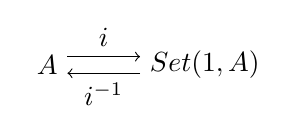
\begin{tikzpicture}[auto]
				\node (a) at (0, 0) {$A$};
				\node (set1a) at (2, 0) {$\arset{Set}{1}{A}$};
				\draw[->,transform canvas={yshift=3pt}] (a) to node{$i$}(set1a);
				\draw[->,transform canvas={yshift=-3pt}] (set1a) to node{$i^{-1}$}(a);
			\end{tikzpicture}
		\end{center}
		すると$\arset{Set}{1}{A}$の任意の元$x$に対し
			\begin{align*}
				(i\circ i^{-1})(x)&=i(i^{-1}(x))&\text{(写像の合成の定義)}\\
				&=i(x(*))&\text{($i^{-1}$の定義)}\\
				&=e_{x(*)}&\text{($i$の定義)}\\
			\end{align*}
		となる。この$\mor{e_{x(*)}}{1}{A}$は$1$の任意の元$*$に対し$e_{x(*)}(*)=x(*)$が成り立つから$i\circ i^{-1}=e_{x(*)}=x$となる。よって$i\circ i^{-1}=id_{\arset{Set}{1}{A}}$が成り立つ。

		また任意の元$\mor{a}{1}{A}$に対し
		\begin{align*}
			(i^{-1}\circ i)(a)&=i^{-1}(i(x))&\text{(写像の合成の定義)}\\
			&=i^{-1}(e_a)&\text{(iの定義)}\\
			&=e_a(*)&\text{($i^{-1}$の定義)}\\
			&=a&\text{($e_a$の定義)}
		\end{align*}
		となる。よって$i^{-1}\circ i=id_A$が成り立つ。

		よって$i\circ i^{-1}=id_{\arset{Set}{1}{A}},\ i^{-1}\circ i=id_A$が示せたので$A\cong\arset{Set}{1}{A}$が成り立つ。

		圏論において一般的な射を取る操作、つまり$\arset{Set}{1}{A}$の元をとる操作が、$A$の元との一対一対応によって$A$の元を取る操作とみなせるということである。

	\end{proof}
	\section{関手}
	これまでの議論はすべて一つの圏の上で行われてきたが、これからはある圏とまた別の圏の関係について考えていく。
	\begin{define}
		ある圏$\cat{C}$からある圏$\cat{D}$への関手$\functor{F}{C}{D}$は以下の関数と公理から構成される。
		また例として、以下の射と対象で構成される圏$\cat{C},\cat{D}$と二つの関手$\functor{T}{C}{D}$、$\functor{S}{C}{D}$を見ていく。
		\begin{center}
			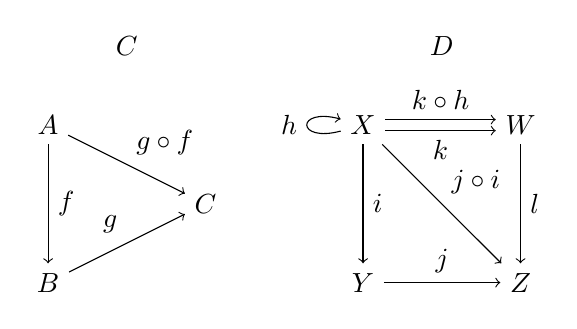
\begin{tikzpicture}[auto]
				\node (a) at (0, 2) {$A$};
				\node (b) at (0, 0) {$B$};
				\node (c) at (2, 1) {$C$};
				\draw[->] (a) to node{$f$}(b);
				\draw[->] (b) to node{$g$}(c);
				\draw[->] (a) to node{$g\circ f$}(c);

				\node (x) at (4, 2) {$X$};
				\node (y) at (4, 0) {$Y$};
				\node (w) at (6, 2) {$W$};
				\node (z) at (6, 0) {$Z$};
				\draw[->] (x) to node{$i$}(y);
				\draw[->] (y) to node{$j$}(z);
				\draw[->] (x) to node{$j\circ i$}(z);
				\draw[->] (w) to node{$l$}(z);
				\draw[->,transform canvas={yshift=-2pt}] (x) to node[swap]{$k$}(w);
				\draw[->,transform canvas={yshift=2pt}] (x) to node{$k\circ h$}(w);
				\draw[->,loop left ,looseness=10] (x) to node{$h$}(x);

				\node (catc) at (1, 3) {$\cat{C}$};
				\node (catd) at (5, 3) {$\cat{D}$};
				%\draw[->,bend right = 15] (catc) to node{$T$}(catd);
				%\draw[->,bend left = 15] (catc) to node{$S$}(catd);
			\end{tikzpicture}
		\end{center}
		\begin{quote}
			\begin{description}
		\item[対象関数]$\cat{C}$の対象$A$に$\cat{D}$の対象$FA$を割り当てる対象関数\[\mor{F}{\obj{C}}{\obj{D}}\]
		そして関手$T$の対象関数$T$を\[T(A)=X,\ T(B)=Y,\ T(C)=Z\]と定義する。
		また関手$S$の対象関数$S$を\[S(A)=X,\ S(B)=X,\ S(C)=W\]と定義する。
		\item[射関数]$\cat{C}$の任意の各対象$A,B$において射$\mor{f}{A}{B}$に圏$\cat{D}$の射$\mor{Ff}{FA}{FB}$を割り当てる射関数\[\mor{F_{A,B}}{\arset{C}{A}{B}}{\arset{D}{FA}{FB}}\]対象$A,B$に対してそれぞれ存在する射関数$F_{A,B}$を総称して$F$と呼ぶことにする。

		つまり、圏$\cat{C}$に含まれる任意の射$\mor{f}{A}{B}$、$\mor{k}{X}{Y}$に対して\[F(f)=F_{A,B}(f)\]\[F(k)=F_{X,Y}(k)\]と置き換えてほしい。
		また対象関数と射関数は記法で区別しないことと、$Tf,TA$ののように括弧を省略する場合もある。

		関手$T$の射関数$T$を\[T(f)=i,\ T(g)=j,\ T(g\circ f)=j\circ i\]と定義する。また各対象の恒等射の対応は
		\begin{align*}
			T(id_A)&=id_{TA}\\
			&=id_{X} \text{($TA=X$)}\\
			T(id_B)&=id_{TB}\\
			&=id_{Y} \text{($TB=Y$)}\\
			T(id_C)&=id_{TC}\\
			&=id_{Z} \text{($TC=Z$)}
		\end{align*}とする。
		\begin{center}
			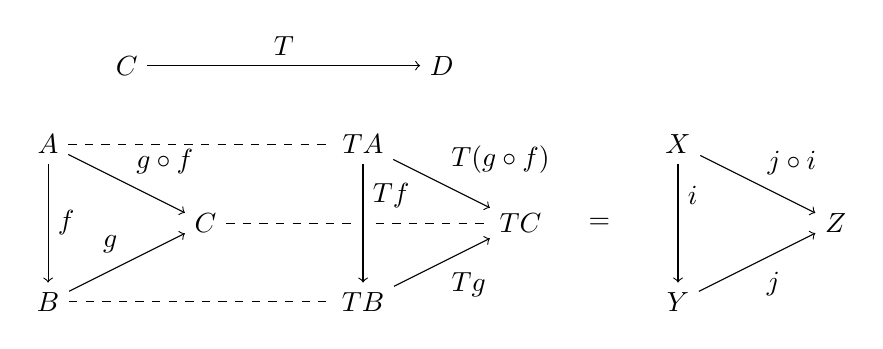
\begin{tikzpicture}[auto]
				\node (a) at (0, 2) {$A$};
				\node (b) at (0, 0) {$B$};
				\node (c) at (2, 1) {$C$};
				\node (ta) at (4, 2) {$TA$};
				\node (tb) at (4, 0) {$TB$};
				\node (tc) at (6, 1) {$TC$};
				\node (x) at (8, 2) {$X$};
				\node (y) at (8, 0) {$Y$};
				\node (z) at (10, 1) {$Z$};

				\node (e) at (7, 1) {$=$};

				\draw[-,dashed] (a) to (ta);
				\draw[-,dashed] (b) to (tb);
				\draw[-,dashed] (c) to (tc);

				\draw[->] (a) to node{$f$}(b);
				\draw[->] (b) to node{$g$}(c);
				\draw[->] (a) to node{$g\circ f$}(c);

				\draw[-, line width=4pt,draw=white] (x) to (y);
				\draw[->] (x) to node[yshift =10]{$i$}(y);
				\draw[->] (y) to node[swap]{$j$}(z);
				\draw[->] (x) to node{$j\circ i$}(z);

				\draw[-, line width=4pt,draw=white] (ta) to (tb);
				\draw[->] (ta) to node[yshift =10]{$Tf$}(tb);
				\draw[->] (tb) to node[swap]{$Tg$}(tc);
				\draw[->] (ta) to node{$T(g\circ f)$}(tc);

				\node (catc) at (1, 3) {$\cat{C}$};
				\node (catd) at (5, 3) {$\cat{D}$};
				\draw[->] (catc) to node{$T$}(catd);

			\end{tikzpicture}
		\end{center}
		この図での点線は対象の写像的な対応を表しているのであって、実際に射が存在するわけではないことに注意してほしい。

		関手$S$の射関数$S$を\[S(f)=h,\ S(g)=k,\ S(g\circ f)=k\circ h\]と定義する。
		恒等射の対応は
		\begin{align*}
			S(id_A)&=id_{SA}\\
			&=id_{X} \text{($SA=X$)}\\
			S(id_B)&=id_{SB}\\
			&=id_{X} \text{($SB=X$)}\\
			S(id_C)&=id_{SC}\\
			&=id_{W} \text{($SC=W$)}
		\end{align*}
		とする。
		\begin{center}
			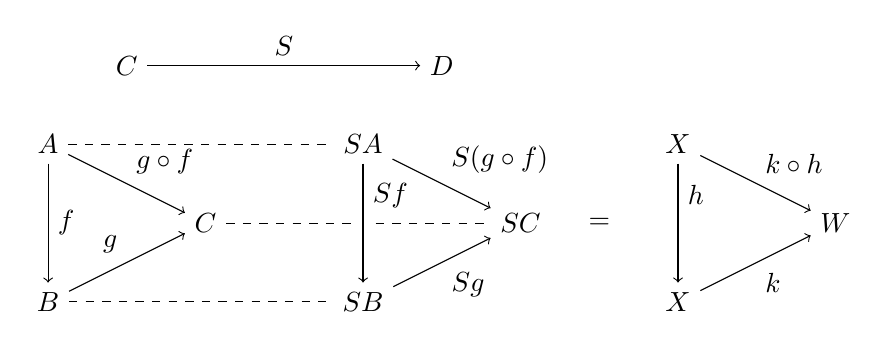
\begin{tikzpicture}[auto]
				\node (a) at (0, 2) {$A$};
				\node (b) at (0, 0) {$B$};
				\node (c) at (2, 1) {$C$};
				\node (ta) at (4, 2) {$SA$};
				\node (tb) at (4, 0) {$SB$};
				\node (tc) at (6, 1) {$SC$};
				\node (x) at (8, 2) {$X$};
				\node (y) at (8, 0) {$X$};
				\node (z) at (10, 1) {$W$};

				\node (e) at (7, 1) {$=$};

				\draw[-,dashed] (a) to (ta);
				\draw[-,dashed] (b) to (tb);
				\draw[-,dashed] (c) to (tc);

				\draw[->] (a) to node{$f$}(b);
				\draw[->] (b) to node{$g$}(c);
				\draw[->] (a) to node{$g\circ f$}(c);

				\draw[-, line width=4pt,draw=white] (x) to (y);
				\draw[->] (x) to node[yshift =10]{$h$}(y);
				\draw[->] (y) to node[swap]{$k$}(z);
				\draw[->] (x) to node{$k\circ h$}(z);

				\draw[-, line width=4pt,draw=white] (ta) to (tb);
				\draw[->] (ta) to node[yshift =10]{$Sf$}(tb);
				\draw[->] (tb) to node[swap]{$Sg$}(tc);
				\draw[->] (ta) to node{$S(g\circ f)$}(tc);

				\node (catc) at (1, 3) {$\cat{C}$};
				\node (catd) at (5, 3) {$\cat{D}$};
				\draw[->] (catc) to node{$S$}(catd);

			\end{tikzpicture}
		\end{center}
		\item[恒等射の保存] 射関数は圏$\cat{C}$の恒等射を$\cat{D}$の恒等射に対応させる。つまり$F(id_A)=id_{FA}$が成り立つ。

		関手$T,S$でも定義を見れば成り立つことがすぐに分かる。
		\item[射の合成の保存]$\cod(f)=\dom(g)$であるとき、$F(g\circ f)=Fg\circ Ff$が成り立つ。

		関手$T,S$においてそれぞれ
		\begin{align*}
			T(g\circ f)&=j\circ i&\text{($T(g\circ f)$の定義)}\\
			&=Tg\circ Tf&\text{($Tg,Tf$の定義)}\\
			S(g\circ f)&=k\circ h&\text{($S(g\circ f)$の定義)}\\
			&=Sg\circ Sf&\text{($Sg,Sf$の定義)}
		\end{align*}
		が成り立つから射の合成を保つことがわかる。
		\end{description}
		\end{quote}
	\end{define}
	\begin{prop}[図式の圏論的な定義]
		添字圏と呼ばれる圏$\cat{J}$から図式を取りたい圏$\cat{C}$への関手は図式である。
		例えば以下のように対象$I,J,K$と射$i,j$で構成される添字圏$J$を図式の骨組み、関手$\functor{F}{I}{C}$を図式の骨組みに圏$C$の対象と射を割り当てる操作とする。

		実際に図式に求められる性質は関手の定義によって満たされることがわかる。
		\begin{center}
			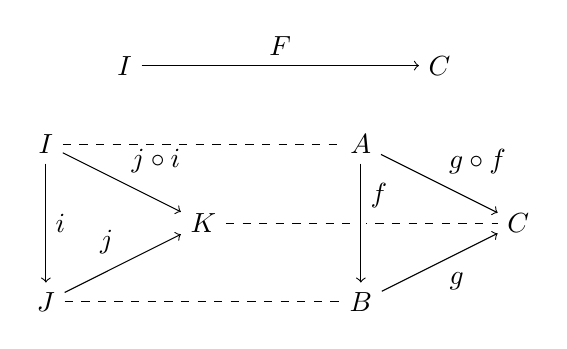
\begin{tikzpicture}[auto]
				\node (a) at (0, 2) {$I$};
				\node (b) at (0, 0) {$J$};
				\node (c) at (2, 1) {$K$};
				\node (x) at (4, 2) {$A$};
				\node (y) at (4, 0) {$B$};
				\node (z) at (6, 1) {$C$};
				\draw[-,dashed] (a) to (x);
				\draw[-,dashed] (b) to (y);
				\draw[-,dashed] (c) to (z);

				\draw[->] (a) to node{$i$}(b);
				\draw[->] (b) to node{$j$}(c);
				\draw[->] (a) to node{$j\circ i$}(c);

				\draw[-, line width=4pt,draw=white] (x) to (y);
				\draw[->] (x) to node[yshift =10]{$f$}(y);
				\draw[->] (y) to node[swap]{$g$}(z);
				\draw[->] (x) to node{$g\circ f$}(z);
				\node (catc) at (1, 3) {$\cat{I}$};
				\node (catd) at (5, 3) {$\cat{C}$};
				\draw[->] (catc) to node{$F$}(catd);

			\end{tikzpicture}
		\end{center}
	\end{prop}
	このように関手は考えている圏の特定の対象や射をピックアップすることが可能である。
	\begin{define}[積関手]
		圏$\cat{C}$が積を持つとき、以下の関数で構成されるある対象$B$に対して圏$C$から圏$C$への関手$\functor{-\times B}{C}{C}$を積関手と呼ぶ。
		\begin{quote}
			\begin{description}
			\item[対象関数] 対象関数を$(-\times B)(A)=A\times B$と定義する。
			\item[射関数] 圏$C$の任意の対象$A,A'$に対する関数$(-\times B)_{A,A'}$を任意の射$\mor{f}{A}{A'}$に対して
			\begin{align*}
				(-\times B)_{A,A'}(f)&=\mor{f\times id_B}{(-\times B)(A)}{(-\times B)(A)}\\
				&=\mor{f\times id_B}{A\times B}{A'\times B}
			\end{align*}
			と定義する。同様に任意の対象$A,A'$に対して存在する射関数$(-\times B)_{A,A'}$を総称して$(-\times B)$と呼ぶ。
			\begin{center}
				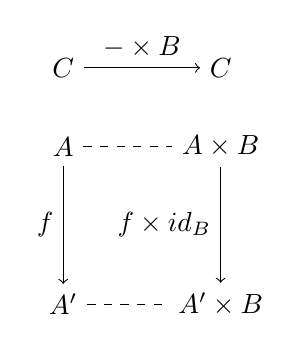
\begin{tikzpicture}[auto]
					\node (a) at (0, 2) {$A$};
					\node (a') at (0, 0) {$A'$};
					\node (ab) at (2, 2) {$A\times B$};
					\node (a'b) at (2, 0) {$A'\times B$};
					\node (catc1) at (0, 3) {$\cat{C}$};
					\node (catc2) at (2, 3) {$\cat{C}$};
					\draw[-,dashed] (a) to (ab);
					\draw[-,dashed] (a') to (a'b);

					\draw[->] (catc1) to node{$-\times B$}(catc2);
					\draw[->] (a) to node[swap]{$f$}(a');
					\draw[->] (ab) to node[swap]{$f\times id_B$}(a'b);
				\end{tikzpicture}
			\end{center}
			\item[恒等射の保存] 射影射の対が恒等射になることを用いて$(-\times B)(id_A)=id_{(-\times B)(A)}$を示せばよい。
			\begin{align*}
				(-\times B)(id_A)&=id_A\times id_B&\text{(射関数の定義)}\\
				&=\tuple{id_A\circ\pi_A,id_B\circ\pi_B}&\text{(射の積の定義)}\\
				&=\tuple{\pi_A,\pi_B}&\text{(恒等射の性質)}\\
				&=id_{A\times B}&\text{(射影射の対)}\\
				&=id_{(-\times B)(A)}&\text{(対象関数の定義)}
			\end{align*}
			よって積関手は恒等射を保つことが示せた。
			\item[射の合成の保存]任意の対象$A,A',A''$と任意の射$\mor{f}{A}{A'},\mor{f'}{A'}{A''}$に対して\[(-\times B)(f'\circ f)=(-\times B)(f')\circ(-\times B)(f)\]が成り立つことを、積と合成の交換から示す。
			\begin{align*}
				(-\times B)(f'\circ f)&=(f'\circ f)\times id_B&\text{(射関数の定義)}\\
				&=(f'\circ f)\times (id_B\circ id_B)&\text{(恒等射の性質)}\\
				&=(f'\times id_B)\circ(f\times id_B)&\text{(積と合成の交換)}\\
				&=(-\times B)(f')\circ(-\times B)(f)&\text{(射関数の定義)}
			\end{align*}
			\begin{center}
				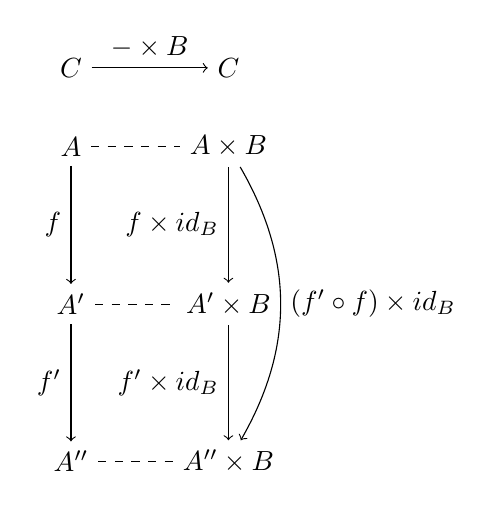
\begin{tikzpicture}[auto]
					\node (a) at (0, 2) {$A$};
					\node (a') at (0, 0) {$A'$};
					\node (a'') at (0, -2) {$A''$};
					\node (ab) at (2, 2) {$A\times B$};
					\node (a'b) at (2, 0) {$A'\times B$};
					\node (a''b) at (2, -2) {$A''\times B$};
					\node (catc1) at (0, 3) {$\cat{C}$};
					\node (catc2) at (2, 3) {$\cat{C}$};
					\draw[-,dashed] (a) to (ab);
					\draw[-,dashed] (a') to (a'b);
					\draw[-,dashed] (a'') to (a''b);
					\draw[->] (catc1) to node{$-\times B$}(catc2);
					\draw[->] (a) to node[swap]{$f$}(a');
					\draw[->] (a') to node[swap]{$f'$}(a'');
					\draw[->] (ab) to node[swap]{$f\times id_B$}(a'b);
					\draw[->] (a'b) to node[swap]{$f'\times id_B$}(a''b);
					\draw[->,bend left =30] (ab) to node{$(f'\circ f)\times id_B$}(a''b);
				\end{tikzpicture}
			\end{center}
			よって積関手は射の合成を保つことが示せた。
		\end{description}
		\end{quote}
	\end{define}
	\begin{prop}[関手の同型の保存]
		任意の圏$\cat{C,D}$と任意の関手$\functor{F}{C}{D}$、圏$\cat{C}$の対象$A,B$において、
		\[A\cong B \Longrightarrow FA\cong FB\]が成り立つ。
	\end{prop}
	\begin{proof}
		同型$A\cong B$のある同型射$\mor{i}{A}{B},\mor{i^{-1}}{B}{A}$に対して$\mor{Fi}{FA}{FB},\mor{Fi^{-1}}{FB}{FA}$も同様に同型射であることを示せばよい。

		\begin{align*}
			Fi^{-1}\circ Fi&=F(i^{-1}\circ i)&\text{($F$の射の合成の保存)}\\
			&=F(id_A)&\text{(恒等射の定義)}\\
			&=id_{FA}&\text{($F$の恒等射の保存)}\\
			Fi\circ Fi^{-1}&=F(i\circ i^{-1})&\text{($F$の射の合成の保存)}\\
			&=F(id_B)&\text{(恒等射の定義)}\\
			&=id_{FB}&\text{($F$の恒等射の保存)}\\
		\end{align*}
		$Fi^{-1}\circ Fi=id_{FA}$、$Fi\circ Fi^{-1}=id_{FB}$より、$Fi,Fi^{-1}$が同型射なる。
		よって$FA\cong FB$が成り立つ。
	\end{proof}


	\subsection{小さい圏の圏}
	関手は圏から圏への一種の写像であるため、圏を対象とし関手を射とするような圏である圏の圏を考えることができそうである。
	まずは合成射、恒等射にあたる関手を定義していく。
	\begin{define}[合成関手]
		関手$\functor{F}{C}{C'}$、$\functor{G}{C'}{C''}$を合成した関手$\functor{G\circ F}{C}{C'}$を以下の要素によって定義する。
		\begin{quote}
			\begin{description}
			\item[対象関数]関手$F,G$のそれぞれの対象関数$F,G$に対して$G\circ F$の対象関数を$G\circ F$と定義する。つまり圏$\cat{C}$の任意の対象$A$に対して\[(G\circ F)(A)=G(FA)\]となるような写像である。
			\item[射関数]関手$F,G$のそれぞれの射関数$F,G$に対して$G\circ F$の射関数を$G\circ F$と定義する。
			つまり圏$\cat{C}$の任意の対象$A,A'$と任意の射$\mor{f}{A}{A'}$に対して\[\mor{(G\circ F)_{}(f)=G(Ff)}{GFA}{GF{A'}}\]となるような写像である。

			各二対象ごとの射関数も見ていくと、関手$F,G$のそれぞれの関数\[\mor{F_{A,A'}}{\arset{C}{A}{A'}}{\arset{C'}{FA}{FA'}}\]\[\mor{G_{FA,FA'}}{\arset{C'}{FA}{FA'}}{\arset{C''}{GFA}{GFA'}}\]に対して$G\circ F$の関数を\[(G\circ F)_{A,A'}=\mor{G_{FA,FA'}\circ F_{A,A'}}{\arset{C}{A}{A'}}{\arset{C''}{GFA}{GFA'}}\]となる。このように関手の合成はそれぞれの関手の対象関数、射関数の合成に還元して考える。

			\begin{center}
				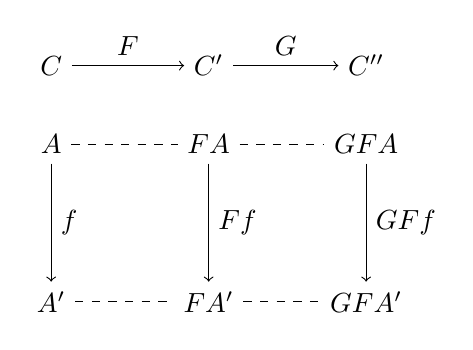
\begin{tikzpicture}[auto]
					\node (a) at (0, 2) {$A$};
					\node (a') at (0, 0) {$A'$};
					\node (fa) at (2, 2) {$FA$};
					\node (fa') at (2, 0) {$FA'$};
					\node (gfa) at (4, 2) {$GFA$};
					\node (gfa') at (4, 0) {$GFA'$};
					\node (catc) at (0, 3) {$\cat{C}$};
					\node (catc') at (2, 3) {$\cat{C'}$};
					\node (catc'') at (4, 3) {$\cat{C''}$};
					\draw[-,dashed] (a) to (fa);
					\draw[-,dashed] (a') to (fa');
					\draw[-,dashed] (fa) to (gfa);
					\draw[-,dashed] (fa') to (gfa');
					\draw[->] (catc) to node{$F$}(catc');
					\draw[->] (catc') to node{$G$}(catc'');

					\draw[->] (a) to node{$f$}(a');
					\draw[->] (fa) to node{$Ff$}(fa');
					\draw[->] (gfa) to node{$GFf$}(gfa');

				\end{tikzpicture}
			\end{center}
			また紛らわしくない場合は合成関手$G\circ F$を$GF$と略すことにする。
			\item[恒等射の保存] $GF(id_A)=id_{GFA}$を示せばよい。
				\begin{align*}
					GF(id_A)&=G(F(id_A))&\text{(射関数の定義)}\\
					&=G(id_{FA})&\text{(関手$F$の恒等射の保存)}\\
					&=id_{GFA}&\text{(関手$G$の恒等射の保存)}
				\end{align*}
			よって合成関手は恒等射を保つ。
			\item[射の合成の保存] $GF(g\circ f)=GFg\circ GFf$を示せばよい。
				\begin{align*}
					GF(g\circ f)&=G(F(g\circ f))&\text{(射関数の定義)}\\
					&=G(Fg\circ Ff)&\text{(関手$F$の射の合成の保存)}\\
					&=GFg\circ GFf&\text{(関手$G$の射の合成の保存)}
				\end{align*}
			よって合成関手は射の合成を保つ。
			\begin{center}
				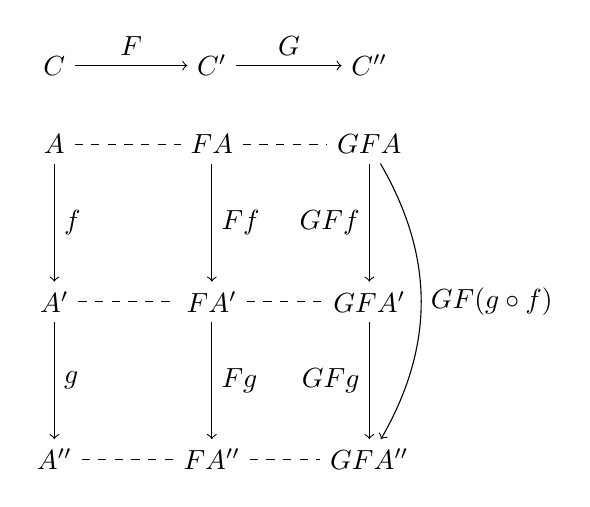
\begin{tikzpicture}[auto]
					\node (a) at (0, 2) {$A$};
					\node (a') at (0, 0) {$A'$};
					\node (a'') at (0, -2) {$A''$};
					\node (fa) at (2, 2) {$FA$};
					\node (fa') at (2, 0) {$FA'$};
					\node (fa'') at (2, -2) {$FA''$};
					\node (gfa) at (4, 2) {$GFA$};
					\node (gfa') at (4, 0) {$GFA'$};
					\node (gfa'') at (4, -2) {$GFA''$};
					\node (catc) at (0, 3) {$\cat{C}$};
					\node (catc') at (2, 3) {$\cat{C'}$};
					\node (catc'') at (4, 3) {$\cat{C''}$};
					\draw[-,dashed] (a) to (fa);
					\draw[-,dashed] (a') to (fa');
					\draw[-,dashed] (a'') to (fa'');
					\draw[-,dashed] (fa) to (gfa);
					\draw[-,dashed] (fa') to (gfa');
					\draw[-,dashed] (fa'') to (gfa'');
					\draw[->] (catc) to node{$F$}(catc');
					\draw[->] (catc') to node{$G$}(catc'');

					\draw[->] (a) to node{$f$}(a');
					\draw[->] (a') to node{$g$}(a'');

					\draw[->] (fa) to node{$Ff$}(fa');
					\draw[->] (fa') to node{$Fg$}(fa'');

					\draw[->] (gfa) to node[swap]{$GFf$}(gfa');
					\draw[->] (gfa') to node[swap]{$GFg$}(gfa'');
					\draw[->,bend left =30] (gfa) to node{$GF(g\circ f)$}(gfa'');
				\end{tikzpicture}
			\end{center}
		\end{description}
		\end{quote}
	\end{define}
	\begin{define}[恒等関手]
		任意の圏$\cat{C}$の恒等関手$\functor{Id_{\cat{C}}}{C}{C}$を以下の要素で定義する。
		\begin{quote}
			\begin{description}
				\item[対象関数] 対象関数を恒等写像$Id_{\cat{C}}(A)=A$と定義する。
				\item[射関数] 射関数を恒等写像$Id_{\cat{C}}(f)=f$と定義する。
				\item[恒等射の保存] $Id_{\cat{C}}(id_C)=id_C=id_{Id_{\cat{C}}(C)}$より恒等射を保つ
				\item[射の合成の保存] $Id_{\cat{C}}(g\circ f)=g\circ f=Id_{\cat{C}}(g)\circ Id_{\cat{C}}(f)$より射の合成を保つ。
			\end{description}
		\end{quote}
	\end{define}
	\begin{define}[小さい圏の圏]
		小さい圏の圏$\cat{Cat}$は以下の要素で構成される。

		集合の圏の時と同様に、小さい圏の「小さい」とは簡単に説明をするのであれば自己言及を防ぐための条件付けであり、実際に$\cat{Cat}$は小さい圏ではないため$\cat{Cat}$の対象にはならない。
		\begin{quote}
			\begin{description}
				\item[対象] 任意の小さい圏
				\item[射] 任意の小さい圏$\cat{A,B}$の間の任意の関手$\functor{F}{A}{B}$
				\item[射の合成] 関手$\functor{F}{C}{C'}$、$\functor{G}{C'}{C''}$に対して合成した関手$\functor{G\circ F}{C}{C'}$をとる操作を射の合成とする。
				\item[恒等射の存在]任意の圏$\cat{A}$の恒等関手$Id_{\cat{A}}$を恒等射とする。
				\item[結合律]
				$H\circ (G\circ F)=(H\circ G)\circ F$が合成可能な任意の関手$F,G,H$で成り立つことを示せばよい。
				二つの関手が等しいことを示すにはそれぞれを構成する対象関数と射関数が等しいことを示せばよい。
				対象関数については、関手$F,G,H$の対象関数$F,G,H$に対して$H\circ (G\circ F)=(H\circ G)\circ F$は明らかに成り立つ。
				射関数についても写像の結合律に還元すると、
				\begin{align*}
					(H\circ (G\circ F))_{A,A'}&=H_{GFA,GFA'}\circ (G\circ F)_{A,A}&\text{(射関数の合成の定義)}\\
					&=H_{GFA,GFA'}\circ (G_{FA,FA'}\circ F_{A,A'})&\text{(射関数の合成の定義)}\\
					&=(H_{GFA,GFA'}\circ G_{FA,FA'})\circ F_{A,A'}&\text{(写像の結合則)}\\
					&=(H\circ G)_{FA,FA'}\circ F_{A,A'}&\text{(射関数の合成の定義)}\\
					&=(H\circ (G\circ F))_{A,A'}&\text{(射関数の合成の定義)}
				\end{align*}
				となり、射関数においても結合則が成り立つ。
				\item[単位元律]
				任意の圏$\cat{C}$の恒等関手$Id_{\cat{C}}$と任意の関手$\functor{F}{X}{C}$、$\functor{G}{C}{Y}$において$Id_{\cat{C}}\circ F=F$、$G\circ Id_{\cat{C}}=G$が成り立つことを示せばよい。

				恒等関手の対象関数、射関数ともに恒等写像
				\[\mor{Id_\cat{C}=id_{\obj{A}}}{\obj{A}}{\obj{A}}\]
				\[\mor{Id_{\cat{C}A,A'}=id_{\arset{C}{A}{A'}}}{\arset{C}{A}{A'}}{\arset{C}{A}{A'}}\]
				となるため、写像の単位元律より$Id_{\cat{C}}\circ F=F$、$G\circ Id_{\cat{C}}=G$が成り立ち単位元律が成り立つ。
			\end{description}
		\end{quote}
	\end{define}
	\subsection{積圏と一点離散圏}
	\begin{define}[積圏]
		ある圏$\cat{A,B}$に対する積圏$\cat{A\times B}$を以下の要素で定義する。
		\begin{quote}
			\begin{description}
				\item[対象] \[\obj{A\times B}=\obj{A}\times\obj{B}\]

				すなわち、圏$\cat{A}$と圏$\cat{B}$の任意の対象$A,B$の対$\tuple{A,B}$が$\cat{A\times B}$の対象であり、紛らわしくないように\[\tuple{A,B}=\pcobj{A,B}\]と表記する。

				また$\obj{A}\times\obj{B}$は直積集合であり、集合の圏の積対象であるが、対象$\pcobj{A,B}$そのものは積の普遍性を持たないことに注意してほしい。今回積とみなすのは対象ではなく圏の方である。
				\item[射] 任意の対象$\pcobj{A,B},\pcobj{A',B'}$に対してその射集合をそれぞれ\[\arset{(A\times B)}{\pcobj{A,B}}{\pcobj{A',B'}}=\arset{A}{A}{A'}\times\arset{B}{B}{B'}\]と定義する。

				すなわち、圏$\cat{A}$の射$\mor{f}{A}{A'}$と圏$\cat{B}$の射$\mor{g}{B}{B'}$の元の対\[\mor{\tuple{f,g}}{[A,B]}{[A',B']}\]が$\cat{A\times B}$の射であり、対象と同様に\[\tuple{f,g}=\pcobj{f,g}\]と表記する。
				同様に$\arset{A}{A}{A'}\times\arset{B}{B}{B'}$も直積集合であり、集合の圏の積対象である。
				\begin{center}
					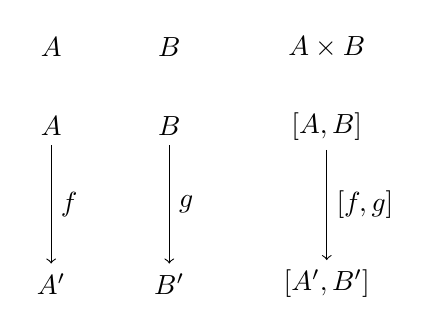
\begin{tikzpicture}[auto]
						\node (a) at (0, 0) {$A$};
						\node (a') at (0, -2) {$A'$};
						\node (b) at (1.5, 0) {$B$};
						\node (b') at (1.5, -2) {$B'$};
						\node (ab) at (3.5, 0) {$\pcobj{A,B}$};
						\node (ab') at (3.5, -2) {$\pcobj{A',B'}$};
						\draw[->] (a) to node{$f$}(a');
						\draw[->] (b) to node{$g$}(b');
						\draw[->] (ab) to node{$\pcobj{f,g}$}(ab');
						\node (cata) at (0, 1) {$\cat{A}$};
						\node (catb) at (1.5, 1) {$\cat{B}$};
						\node (catb) at (3.5, 1) {$\cat{A\times B}$};
					\end{tikzpicture}
				\end{center}
				\item[射の合成] 射$\mor{\pcobj{f,g}}{\pcobj{A,B}}{\pcobj{A',B'}}$と$\mor{\pcobj{f',g'}}{\pcobj{A',B'}}{\pcobj{A'',B''}}$の合成射\[\mor{\pcobj{f',g'}\circ\pcobj{f,g}}{\pcobj{A,B}}{\pcobj{A',B'}}\]を\[\pcobj{f',g'}\circ\pcobj{f,g}=\pcobj{f'\circ f,g'\circ g}\]と定義する。
				\begin{center}
					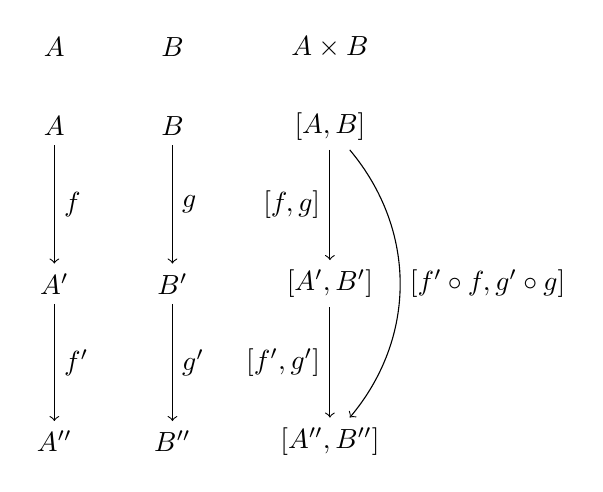
\begin{tikzpicture}[auto]
						\node (a) at (0, 0) {$A$};
						\node (a') at (0, -2) {$A'$};
						\node (a'') at (0, -4) {$A''$};
						\node (b) at (1.5, 0) {$B$};
						\node (b') at (1.5, -2) {$B'$};
						\node (b'') at (1.5, -4) {$B''$};
						\node (ab) at (3.5, 0) {$\pcobj{A,B}$};
						\node (ab') at (3.5, -2) {$\pcobj{A',B'}$};
						\node (ab'') at (3.5, -4) {$\pcobj{A'',B''}$};
						\draw[->] (a) to node{$f$}(a');
						\draw[->] (a') to node{$f'$}(a'');
						\draw[->] (b) to node{$g$}(b');
						\draw[->] (b') to node{$g'$}(b'');
						\draw[->] (ab) to node[swap]{$\pcobj{f,g}$}(ab');
						\draw[->] (ab') to node[swap]{$\pcobj{f',g'}$}(ab'');
						\draw[->,bend left =40] (ab) to node{$\pcobj{f'\circ f,g'\circ g}$}(ab'');
						\node (cata) at (0, 1) {$\cat{A}$};
						\node (catb) at (1.5, 1) {$\cat{B}$};
						\node (catb) at (3.5, 1) {$\cat{A\times B}$};
					\end{tikzpicture}
				\end{center}
				\item[恒等射の存在] 対象$[A,B]$の恒等射$id_{\pcobj{A,B}}$を\[id_{\pcobj{A,B}}=\pcobj{id_A,id_B}\]と定義する。
				\item[結合律]$(\pcobj{f'',g''}\circ\pcobj{f',g'})\circ\pcobj{f,g}=\pcobj{f'',g''}\circ(\pcobj{f',g'}\circ\pcobj{f,g})$を示せばよい。積圏の射の合成の定義を用いて圏の結合律に還元する。
				\begin{align*}
					(\pcobj{f'',g''}\circ\pcobj{f',g'})\circ\pcobj{f,g}&=\pcobj{(f''\circ f')\circ f,(g''\circ g')\circ g}&\text{(積圏の射の合成の定義)}\\
					&=\pcobj{f''\circ (f'\circ f),g''\circ (g'\circ g)}&\text{(圏$\cat{A,B}$の結合則)}\\
					&=\pcobj{f'',g''}\circ(\pcobj{f',g'}\circ\pcobj{f,g})&\text{(積圏の射の合成の定義)}
				\end{align*}
				よって成り立つ。
				\item[単位元律]任意の対象$\pcobj{A,B}$と恒等射$id_{\pcobj{A,B}}$、任意の射$\mor{\pcobj{f,g}}{\pcobj{X,Y}}{\pcobj{A,B}}$、$\mor{\pcobj{f',g'}}{\pcobj{A,B}}{\pcobj{X',Y'}}$において\[id_{\pcobj{A,B}}\circ\pcobj{f,g}=\pcobj{f,g}],\ \pcobj{f',g'}\circ id_{\pcobj{A,B}}=\pcobj{f',g'}\]が成り立つことを示せばよい。同様に積圏の射の合成の定義を用いて圏の結合律に還元する。
				\begin{align*}
					id_{\pcobj{A,B}}\circ\pcobj{f,g}&=\pcobj{id_A,id_B}\circ\pcobj{f,g}&\text{(圏$\cat{A\times B}$の恒等射の定義)}\\
					&=\pcobj{id_A\circ f,id_B\circ g}&\text{(圏$\cat{A\times B}$の射の合成の定義)}\\
					&=\pcobj{f,g}&\text{(圏$\cat{A,B}$の単位元律)}\\
					\pcobj{f',g'}\circ id_{\pcobj{A,B}}&=\pcobj{f',g'}\circ\pcobj{id_A,id_B}&\text{(圏$\cat{A\times B}$の恒等射の定義)}\\
					&=\pcobj{f'\circ id_A,g'\circ id_B}&\text{(圏$\cat{A\times B}$の射の合成の定義)}\\
					&=\pcobj{f',g'}&\text{(圏$\cat{A,B}$の単位元律)}
				\end{align*}
				よって単位元律が成り立つ。
			\end{description}
		\end{quote}
	\end{define}


	\begin{define}[射影関手]
		関手$\functor{\Pi_{LA}}{A\times B}{A}$を以下の写像で定義する。また射影射と同様に紛らわしくない場合に$\Pi_{LA}=\Pi_A$と表記する。
		\begin{quote}
			\begin{description}
				\item[対象関数] 積圏の対象の定義より、圏$\cat{A\times B}$の対象の集合は$\obj{A}\times\obj{B}$である。これを集合の圏における積とみなし、射影写像\[\mor{\Pi_A=\pi_{\obj{A}}}{\obj{A}\times\obj{B}}{\obj{A}}\]を対象関数とする。
				すなわち$\Pi_A(\pcobj{A,B})=A$となるような写像である。
				\item[射関数] 対象関数と同様に射集合$\arset{A}{A}{A'}\times\arset{B}{B}{B'}$の射影写像\[\mor{\Pi_A=\pi_{\arset{A}{A}{A'}}}{\arset{A}{A}{A'}\times\arset{B}{B}{B'}}{\arset{A}{A}{A'}}\]を射関数とする。
				すなわち$\Pi_A(\pcobj{f,g})=f$となるような写像である。
				\item[恒等射の保存] $\Pi_A(id_{A\times B})=\Pi_A(\pcobj{id_A,id_B})=id_A$より恒等射を保つ
				\item[射の合成の保存]元の圏の結合則に還元する。
				\begin{align*}
					\Pi_A(\pcobj{f',g'}\circ\pcobj{f,g})&=\Pi_A(\pcobj{f'\circ f, g'\circ g})&\text{($\cat{A\times B}$の射の合成の定義)}\\
					&=f'\circ f&\text{(射関数の定義)}\\
					&=\Pi_A(\pcobj{f',g'})\circ\Pi_A(\pcobj{f,g})&\text{(射関数の定義)}
				\end{align*}
				よって射の合成を保つ。
			\end{description}
		\end{quote}
	\end{define}
	また同様に$\functor{\Pi_{RB}}{A\times B}{B}$も定義できる。
	\begin{define}[関手の対]
		関手$\functor{F}{X}{A}$と$\functor{G}{X}{B}$の対$\functor{\tuple{F,G}}{X}{A\times B}$を以下の写像で定義する。
		\begin{quote}
			\begin{description}
				\item[対象関数] 関手$F,G$の対象関数$\mor{F}{\obj{X}}{\obj{A}}$、$\mor{G}{\obj{X}}{\obj{B}}$の対
				\begin{align*}
					&\mor{\tuple{F,G}}{\obj{X}}{\obj{A\times B}}\\
					=&\mor{\tuple{F,G}}{\obj{X}}{\obj{A}\times \obj{B}}
				\end{align*}
				を対象関数とする。
				すなわち圏$\cat{X}$の対象$X$に対して$\tuple{F,G}(X)=\pcobj{FX,GX}$となるような写像である。
				\item[射関数]
				関手$F,G$の対象$X,X'$に対する射関数$\mor{F_{X,X'}}{\arset{X}{X}{X'}}{\arset{A}{FX}{FX'}},\ \mor{G_{X,X'}}{\arset{X}{X}{X'}}{\arset{B}{GX}{GX'}}$の対
				\begin{align*}
					&\mor{\tuple{F,G}_{X,X'}&&}{\arset{X}{X}{X'}}{\arset{A\times B}{\tuple{FX,GX}}{\tuple{FX',GX'}}}\\
					=&	\mor{\tuple{F_{X,X'},G_{X,X'}}&&}{\arset{X}{X}{X'}}{\arset{A}{FX}{FX'}\times\arset{B}{GX}{GX'}}
				\end{align*}
				を射関数とする。
				すなわち射$\mor{f}{X}{X'}$に対して\[\mor{\tuple{F,G}(f)=\pcobj{Ff,Gf}}{\pcobj{FX,GX}}{\pcobj{FX',GX'}}\]となるような写像である。

				\begin{center}
					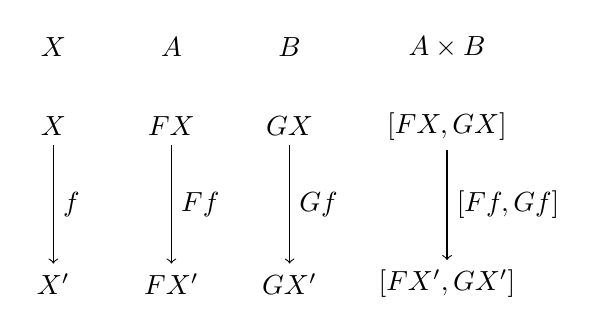
\begin{tikzpicture}[auto]
						\node (x) at (-1.5, 0) {$X$};
						\node (x') at (-1.5, -2) {$X'$};
						\node (a) at (0, 0) {$FX$};
						\node (a') at (0, -2) {$FX'$};
						\node (b) at (1.5, 0) {$GX$};
						\node (b') at (1.5, -2) {$GX'$};
						\node (ab) at (3.5, 0) {$[FX,GX]$};
						\node (ab') at (3.5, -2) {$[FX',GX']$};
						\draw[->] (x) to node{$f$}(x');
						\draw[->] (a) to node{$Ff$}(a');
						\draw[->] (b) to node{$Gf$}(b');
						\draw[->] (ab) to node{$[Ff,Gf]$}(ab');
						\node (cata) at (-1.5, 1) {$\cat{X}$};
						\node (cata) at (0, 1) {$\cat{A}$};
						\node (catb) at (1.5, 1) {$\cat{B}$};
						\node (catb) at (3.5, 1) {$\cat{A\times B}$};
					\end{tikzpicture}
				\end{center}
				\item[恒等射の保存]
				\begin{align*}
					\tuple{F,G}(id_X)&=\pcobj{F(id_X),G(id_X)}&\text{(射関数の定義)}\\
					&=\pcobj{id_{FX},id_{GX}}&\text{($F,G$の恒等射の保存)}\\
					&=id_{\pcobj{FX,GX}}&\text{(積圏の恒等射の定義)}
				\end{align*}
			よって恒等射を保つ
				\item[射の合成の保存]
				\begin{align*}
					\tuple{F,G}(f'\circ f)&=\pcobj{F(f'\circ f),G(f'\circ f)}&\text{(射関数の定義)}\\
					&=\pcobj{Ff'\circ Ff, Gf'\circ Gf}&\text{($F,G$の射の合成の保存)}\\
					&=\pcobj{Ff',Gf'}\circ\pcobj{Ff,Gf}&\text{(積圏の射の合成の定義)}\\
					&=\tuple{F,G}(f')\circ\tuple{F,G}(f)&\text{(射関数の定義)}
				\end{align*}
			よって射の合成を保つ。
			\end{description}
		\end{quote}
	\end{define}
	\begin{prop}
		積圏$\cat{A\times B}$と射影関手$\Pi_A,\Pi_B$の組$(\cat{A\times B},\Pi_A,\Pi_B)$は$\cat{Cat}$における積である。
	\end{prop}
	\begin{proof}
		積$(\cat{A\times B},\Pi_A,\Pi_B)$において、圏$\cat{X}$、関手$\functor{F}{X}{A}$、$\functor{G}{X}{B}$で構成される任意の組$(\cat{X},F,G)$に対して、$\Pi_A\circ\tuple{F,G}=F,\ \Pi_B\circ\tuple{F,G}=G$が成り立つような関手の対$\functor{\tuple{F,G}}{X}{A\times B}$が一意に存在することを示せばよい。
		\begin{center}
			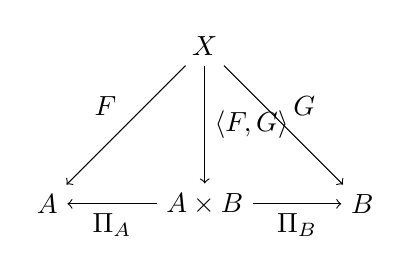
\begin{tikzpicture}[auto]
				\node (a) at (0, 0) {$\cat{A}$};
				\node (ab) at (2, 0) {$\cat{A\times B}$};
				\node (b) at (4, 0) {$\cat{B}$};
				\node (x) at (2, 2) {$\cat{X}$};
				\draw[->] (x) to node[swap]{$F$}(a);
				\draw[->] (x) to node{$G$}(b);
				\draw[->] (ab) to node{$\Pi_A$}(a);
				\draw[->] (ab) to node[swap]{$\Pi_B$}(b);
				\draw[->] (x) to node{$\tuple{F,G}$}(ab);
			\end{tikzpicture}
		\end{center}
		端的に述べるなら積圏、関手の対、射影関手の各々が持つ対象関数、射関数はそれぞれ積対象、射の対、射影射で構成されることから、積の普遍性を満たすことを示すのは難しくない。

		関手$F,G$の対象関数$F,G$、射影関手$\Pi_A,\Pi_B$の対象関数$\pi_{\obj{A}},\pi_{\obj{B}}$、そして関手の対の対象関数$\tuple{F,G}$は、その定義により積の図式となる。
		すなわち対象関数$F,G$に対して対象関数$\tuple{F,G}$は一意に存在する。
		\begin{center}
			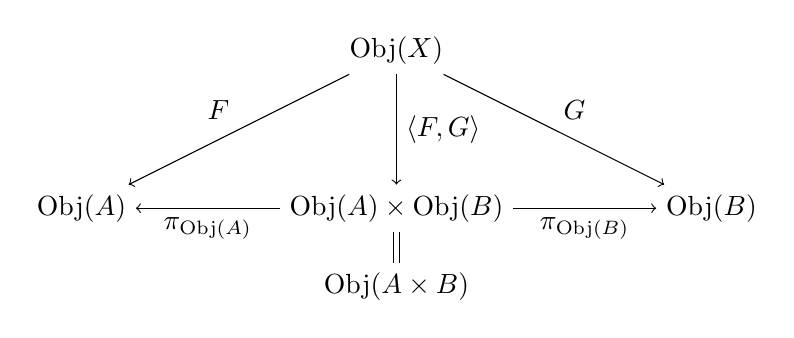
\begin{tikzpicture}[auto]
				\node (a) at (0, 0) {$\obj{A}$};
				\node (ab) at (4, 0) {$\obj{A}\times\obj{B}$};
				\node (abp) at (4, -1) {$\obj{A\times B}$};
				\node (b) at (8, 0) {$\obj{B}$};
				\node (x) at (4, 2) {$\obj{X}$};
				\draw[double distance=2pt] (ab) to (abp);
				\draw[->] (x) to node[swap]{$F$}(a);
				\draw[->] (x) to node{$G$}(b);
				\draw[->] (ab) to node{$\pi_{\obj{A}}$}(a);
				\draw[->] (ab) to node[swap]{$\pi_{\obj{B}}$}(b);
				\draw[->] (x) to node{$\tuple{F,G}$}(ab);
			\end{tikzpicture}
		\end{center}
		各射関数による積の図式は省略するが、同様に射関数$\tuple{F,G}$が一意に存在することが分かる。よって可換性を満たす対象関数と射関数も一意に存在することから、関手の対は積圏における射の対となり、$(\cat{A\times B},\Pi_A,\Pi_B)$は積の普遍性を満たす。
	\end{proof}
	\begin{define}[一点離散圏]
	一つの対象と一つの恒等射で構成される圏$\cat{1}$を一点離散圏とよぶ。
	\end{define}
	\begin{prop}[$\cat{Cat}$の終対象]
		$\cat{1}$は$\cat{Cat}$における終対象である。
	\end{prop}
	\begin{proof}
		任意の圏$\cat{C}$から一点離散圏$\cat{1}$への関手$!_{\cat{C}}$を考える。
		まず$\cat{1}$の対象$*$と射$id_*$は一つしか存在しない。そのため一点集合を$1$として
		\[\obj{1}=1,\ \arset{1}{*}{*}=1\]が成り立つ。

		よって対象関数$!_{\cat{C}}$は
		\begin{align*}
			&\mor{!_{\cat{C}}}{\obj{C}}{\obj{1}}\\
			=&\mor{!_{\cat{C}}}{\obj{C}}{1}
		\end{align*}
		となり一点集合への写像であることがわかる。よって任意の対象$A$に対して$!_{\cat{C}}(A)=*$が成り立ち、このような対象関数が一意に存在することが分かった。

		また任意の二対象$A,B$に対する射関数は
		\begin{align*}
			&\mor{{!_{\cat{C}}}_{A,B}}{\arset{C}{A}{B}}{\arset{1}{!_{\cat{C}}(A)}{!_{\cat{C}}(B)}}\\
			=&\mor{{!_{\cat{C}}}_{A,B}}{\arset{C}{A}{B}}{\arset{1}{*}{*}}\\
			=&\mor{{!_{\cat{C}}}_{A,B}}{\arset{C}{A}{B}}{1}\\
		\end{align*}と書ける。
		よって二対象$A,B$に対する各射関数も一意に存在することが分かった。

		関手$!_{\cat{C}}$の二つの写像が圏$\cat{C}$に対して一意に存在することわかる。
		よって任意の圏$\cat{C}$から一点離散圏$\cat{1}$への関手は一意に存在するから、一点離散圏$\cat{1}$は$\cat{Cat}$における終対象であることが示せた。
	\end{proof}
	\begin{prop}[圏における元]
		任意の圏$\cat{C}$の元、つまり関手$\functor{A}{1}{C}$は圏$\cat{C}$の対象とみなせる。
	\end{prop}
	\begin{proof}
		関手$\functor{A}{1}{C}$は対象関数$\mor{F}{\obj{1}}{\obj{C}}$、射関数$\mor{F}{\arset{1}{*}{*}}{\arset{C}{F(*)}{F(*)}}$で構成される。このとき、$\obj{1}$は一点集合であるから、対象関数$F$は$\obj{C}$の元である。

		また射関数も同様に$\arset{C}{F(*)}{F(*)}$の元であるが、恒等射の保存より写される射は恒等射ただ一つであり、射関数は対象関数に対して一通りにしか定義できないから考慮しなくてもよい。

		よって関手$\functor{A}{1}{C}$は圏$\cat{C}$の対象とみなせる。
	\end{proof}
	積圏$\cat{A\times B}$の対象を$\pcobj{A,B}$と表したが、実際に対象$\functor{A}{1}{A}$と対象$\functor{B}{1}{B}$の関手の対$\functor{\tuple{A,B}}{1}{A\times B}$は$\cat{A\times B}$の対象になる。

	\subsection{特殊な関手}
	対象や射を二つ取るような2変数関数のような関手について考える。
	\begin{define}[双関手]
		積圏からの関手、つまり$\functor{F}{A\times B}{C}$となるような関手を双関手とする。

		また積圏の任意の対象$[A,B]$に対し、\[F(\pcobj{A,B})=F(A,B)\]と略記する。
		さらに積圏の射$\mor{\pcobj{f,id_B}}{\pcobj{A,B}}{\pcobj{A,B'}}$において\[F(\pcobj{f,id_B})=F(f,B)\]と表記する。
	\end{define}
	圏$\cat{A}$の射$f$と圏$\cat{B}$の射$g$がどのように圏$\cat{C}$に写されるのかを以下の可換図式で確認してほしい。
	\begin{center}
		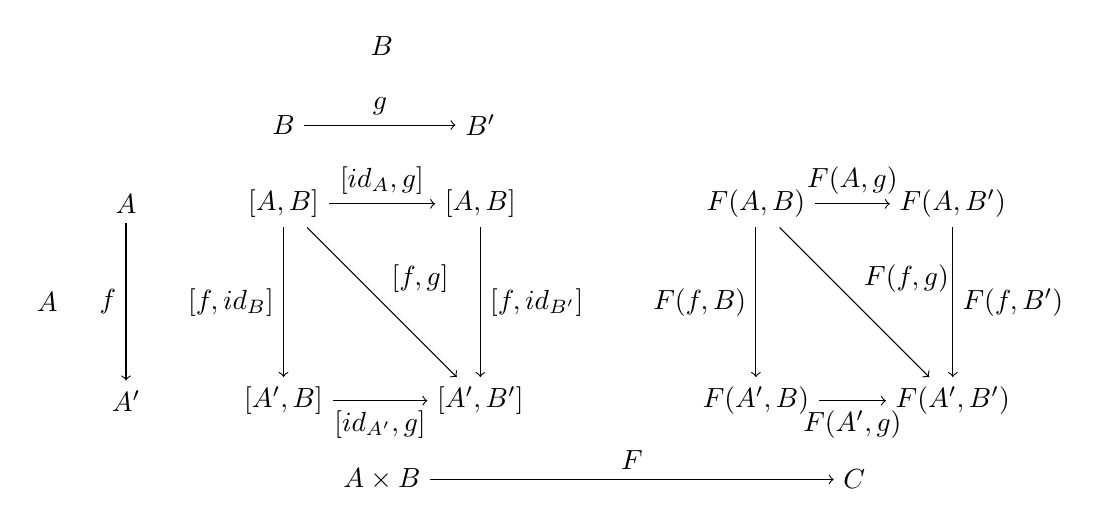
\begin{tikzpicture}[auto]
			\node (a) at (0, 0) {$A$};
			\node (a') at (0, -2.5) {$A'$};
			\node (b) at (2, 1) {$B$};
			\node (b') at (4.5, 1) {$B'$};
			\node (ab) at (2, 0) {$\pcobj{A,B}$};
			\node (a'b) at (2, -2.5) {$\pcobj{A',B}$};
			\node (ab') at (4.5, 0) {$\pcobj{A,B}$};
			\node (a'b') at (4.5, -2.5) {$\pcobj{A',B'}$};

			\node (fab) at (8, 0) {$F(A,B)$};
			\node (fa'b) at (8, -2.5) {$F(A',B)$};
			\node (fab') at (10.5, 0) {$F(A,B')$};
			\node (fa'b') at (10.5, -2.5) {$F(A',B')$};

			\node (cata) at (-1, -1.25) {$\cat{A}$};
			\node (catb) at (3.25, 2) {$\cat{B}$};
			\node (catab) at (3.25, -3.5) {$\cat{A\times B}$};
			\node (catc) at (9.25, -3.5) {$\cat{C}$};

			\draw[->] (a) to node[swap]{$f$}(a');
			\draw[->] (b) to node{$g$}(b');
			\draw[->] (ab) to node[swap]{$\pcobj{f,id_B}$}(a'b);
			\draw[->] (ab') to node{$\pcobj{f,id_{B'}}$}(a'b');
			\draw[->] (ab) to node{$\pcobj{id_A,g}$}(ab');
			\draw[->] (a'b) to node[swap]{$\pcobj{id_{A'},g}$}(a'b');
			\draw[->] (ab) to node{$\pcobj{f,g}$}(a'b');

			\draw[->] (fab) to node[swap]{$F(f,B)$}(fa'b);
			\draw[->] (fab') to node{$F(f,B')$}(fa'b');
			\draw[->] (fab) to node{$F(A,g)$}(fab');
			\draw[->] (fa'b) to node[swap]{$F(A',g)$}(fa'b');
			\draw[->] (fab) to node{$F(f,g)$}(fa'b');
			\draw[->] (catab) to node{$F$}(catc);
		\end{tikzpicture}
	\end{center}
	次に双関手の例として積関手$\functor{-\times B}{C}{C}$を双関手に拡張しようと思う。
	\begin{define}[双積関手]
		積を持つ圏$\cat{C}$上の双積関手$\functor{-\times -}{C\times C}{C}$を以下の写像で定義する。
		\begin{quote}
			\begin{description}
				\item[対象関数] 対象関数を積圏$\cat{C\times C}$の任意の対象$\pcobj{A,B}$に対して\[(-\times -)(A,B)=A\times B\]と定義する。
				\item[射関数] 二対象$\pcobj{A,B},\pcobj{A',B'}$に対する射関数を任意の射$\mor{\pcobj{f,g}}{\pcobj{A,B}}{\pcobj{A',B'}}$に対して\[(-\times -)_{\pcobj{A,B},\pcobj{A',B'}}(f,g)=f\times g\]と定義する。
				\begin{center}
					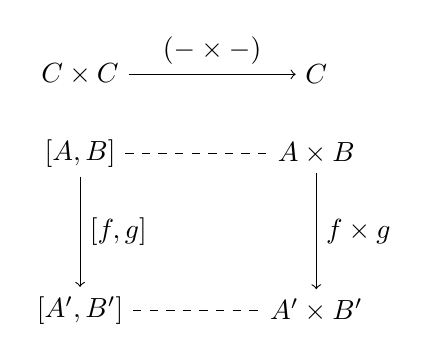
\begin{tikzpicture}[auto]
						\node (ab) at (0, 0) {$\pcobj{A,B}$};
						\node (a'b') at (0, -2) {$\pcobj{A',B'}$};
						\node (pab) at (3, 0) {$A\times B$};
						\node (pa'b') at (3, -2) {$A'\times B'$};
						\node (catcc) at (0, 1) {$\cat{C\times C}$};
						\node (catc) at (3, 1) {$\cat{C}$};
						\draw[-,dashed] (ab) to (pab);
						\draw[-,dashed] (a'b') to (pa'b');
						\draw[->] (ab) to node{$\pcobj{f,g}$}(a'b');
						\draw[->] (pab) to node{$f\times g$}(pa'b');
						\draw[->] (catcc) to node{$(-\times-)$}(catc);
					\end{tikzpicture}
				\end{center}

				\item[恒等射の保存] $(-\times -)(id_{\pcobj{A,B}})=id_{(-\times-)(A,B)}$を示せばよい。
				\begin{align*}
					(-\times -)(id_{\pcobj{A,B}})&=id_A\times id_B&\text{(射関数の定義)}\\
					&=\pcobj{id_A\circ\pi_A,id_B\circ\pi_B}&\text{(射の積の定義)}\\
					&=id_{A\times B}&\text{(射影射の対)}\\
					&=id_{(-\times-)(A,B)}&\text{(対象関数の定義)}
				\end{align*}
				よって恒等射を保つ。
				\item[射の合成の保存] $(-\times -)(f',g')\circ(-\times-)(f,g)=(-\times-)(\pcobj{f',g'}\circ\pcobj{f,g}$を示せばよい。
				\begin{align*}
					(-\times -)(f',g')\circ(-\times-)(f,g)&=(f'\times g')\circ(f\times g)&\text{(射関数の定義)}\\
					&=(f'\circ f)\times(g'\circ g)&\text{(積と合成の交換)}\\
					&=(-\times-)(f'\circ f,g'\circ g)&\text{(射関数の定義)}\\
					&=(-\times-)(\pcobj{f'\circ f,g'\circ g})\\
					&=(-\times-)(\pcobj{f',g'}\circ\pcobj{f,g})&\text{(積圏の射の合成の定義)}
				\end{align*}
				よって射の合成を保つ。
			\end{description}
		\end{quote}
	\end{define}
	対象の積と圏の積が紛らわしいが、まず圏の積の対象$\pcobj{A,B}$は圏$\cat{C}$の$A$と$B$の積が存在しなくとも定義することができ、その点で対象の積$A\times B$より一般的な概念だと考えられる。よってイメージとしては圏$\cat{C}$の外側$\cat{C\times C}$で定義した対象の積もどき$[A,B]$を圏$\cat{C}$に挿入する操作が関手$(-\times-)$と考えられる。ただし、双積関手で写された対象が積の普遍性を満たすかどうかは現段階では説明できない。

	また以前に圏$\cat{C}$の射の積と積圏$\cat{C\times C}$の射の振る舞いが似ていることについて述べたが、実際に関手として二つの射の関係性を示すことができた。
	\begin{define}[双対圏]
		ある圏$\cat{C}$に対する双対圏$\cat{C}^{op}$を以下の要素で定義する。
		\begin{quote}
			\begin{description}
				\item[対象] $\obj{C^{op}}=\obj{C}$とする。

				また圏$\cat{C}$の対象$A$に対応する双対圏$\cat{C^{op}}$の対象も$A$であるが、$\cat{C^{op}}$の対象は$A^{op}$として表記上区別する。
				\item[射] 任意の二対象$A^{op}, B^{op}$に対して射集合を\[\arset{C^{op}}{B^{op}}{A^{op}}=\arset{C}{A}{B}\]と定義する。
				同様に射$\mor{f}{A}{B}$に対応する射を表記上$\mor{f^{op}}{B^{op}}{A^{op}}$とする。
				圏$\cat{C}$と双対圏$\cat{C^{op}}$では射の向きが入れ替わっていることに注意してほしい。
				\begin{center}
					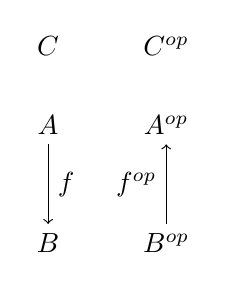
\begin{tikzpicture}[auto]
						\node (a) at (0, 0) {$A$};
						\node (b) at (0, -1.5) {$B$};
						\node (fa) at (1.5, 0) {$A^{op}$};
						\node (fb) at (1.5, -1.5) {$B^{op}$};
						\node (catc) at (0, 1) {$\cat{C}$};
						\node (catd) at (1.5, 1) {$\cat{C^{op}}$};
						\draw[->] (a) to node{$f$}(b);
						\draw[->] (fb) to node{$f^{op}$}(fa);
					\end{tikzpicture}
				\end{center}
				\item[射の合成] 圏$\cat{C}$の射$\mor{f}{A}{B}$、$\mor{g}{B}{C}$の合成射$\mor{g\circ f}{A}{C}$に対して、双対圏$\cat{C}^{op}$の射$\mor{f^{op}}{B^{op}}{A^{op}}$、$\mor{g^{op}}{C^{op}}{B^{op}}$の合成射を
				\[\mor{(g\circ f)^{op}=f^{op}\circ g^{op}}{C^{op}}{A^{op}}\]
				と定義する。
				圏$\cat{C}$と$\cat{C}^{op}$では射の合成の順序が入れ替わっていることに注意してほしい。
				\begin{center}
					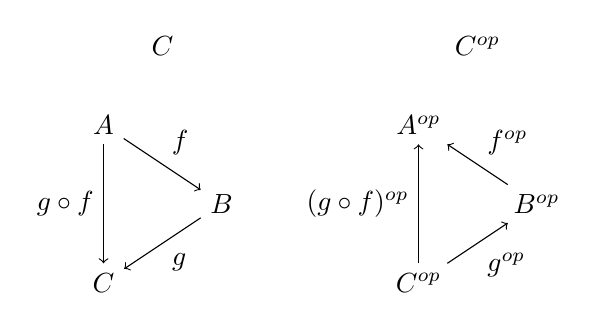
\begin{tikzpicture}[auto]
						\node (a) at (0, 0) {$A$};
						\node (b) at (1.5, -1) {$B$};
						\node (c) at (0, -2) {$C$};
						\node (fa) at (4, 0) {$A^{op}$};
						\node (fb) at (5.5, -1) {$B^{op}$};
						\node (fc) at (4, -2) {$C^{op}$};
						\node (catc) at (0.75, 1) {$\cat{C}$};
						\node (catd) at (4.75, 1) {$\cat{C^{op}}$};
						\draw[->] (a) to node{$f$}(b);
						\draw[->] (b) to node{$g$}(c);
						\draw[->] (a) to node[swap]{$g\circ f$}(c);
						\draw[->] (fb) to node[swap]{$f^{op}$}(fa);
						\draw[->] (fc) to node[swap]{$g^{op}$}(fb);
						\draw[->] (fc) to node{$(g\circ f)^{op}$}(fa);
					\end{tikzpicture}
				\end{center}
				\item[恒等射の存在]圏$\cat{C}$の任意の恒等射$\mor{id_A}{A}{A}$に対して、双対圏$\cat{C}^{op}$の恒等射を\[\mor{(id_A)^{op}=id_{A^{op}}}{A^{op}}{A^{op}}\]と定義する。
				\item[結合律] 合成可能な任意の射$f^{op},g^{op},h^{op}$において、
				\begin{align*}
					(f^{op}\circ g^{op})\circ h^{op}&=(g\circ f)^{op}\circ h^{op}\\
					&=(h\circ(g\circ f))^{op}\\
					&=((h\circ g)\circ f)^{op}\\
					&=f^{op}\circ (h\circ g)^{op}\\
					&=f^{op}\circ (g^{op}\circ h^{op})
				\end{align*}
				となるので結合律を満たす。
				\item[単位元律]任意の恒等射$id_{A^{op}}$、任意の射$\mor{f^{op}}{X^{op}}{A^{op}}$、$\mor{g^{op}}{A^{op}}{Y^{op}}$に対し$id_{A^{op}}\circ f^{op}=f^{op}$、$g^{op}\circ id_{A^{op}}=g^{op}$を示せばよい。
				\begin{align*}
					id_{A^{op}}\circ f^{op}&={id_A}^{op}\circ f^{op}&\text{(双対圏の恒等射の定義)}\\
					&=(f\circ id_A)^{op}&\text{(双対圏の射の合成の定義)}\\
					&=f^{op}&\text{(単位元律)}\\
					g^{op}\circ id_{A^{op}}&=g^{op}\circ {id_A}^{op}&\text{(双対圏の恒等射の定義)}\\
					&=(id_A\circ g)^{op}&\text{(双対圏の射の合成の定義)}\\
					&=g^{op}&\text{(単位元律)}\\
				\end{align*}
				よって単位元律を見たす。
			\end{description}
		\end{quote}
	\end{define}
	次に双対圏のように射の向きを反転させて写すような関手である反変関手を定義する。
	\begin{define}[反変関手]
		圏$\cat{C}$から圏$\cat{D}$への反変関手と呼ばれる圏の間の写像$\functor{F}{C}{D}$を以下の写像と公理で定義する。
		\begin{quote}
			\begin{description}
				\item[対象関数] $\cat{C}$の対象$A$に$\cat{D}$の対象$FA$を割り当てる対象関数\[\mor{F}{\obj{C}}{\obj{D}}\]
				これは通常の関手と同じである。
				\item[射関数] $\cat{C}$の任意の各対象$A,B$において射$\mor{f}{A}{B}$に圏$\cat{D}$の射$\mor{Ff}{FB}{FA}$を割り当てる射関数\[\mor{F_{A,B}}{\arset{C}{A}{B}}{\arset{D}{FB}{FA}}\]対象$A,B$に対してそれぞれ存在する射関数$F_{A,B}$を総称して$F$と呼ぶことにする。
				\begin{center}
					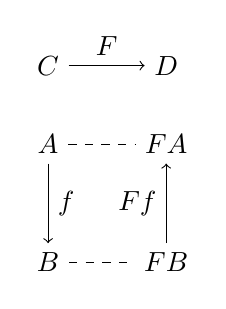
\begin{tikzpicture}[auto]
						\node (a) at (0, 0) {$A$};
						\node (b) at (0, -1.5) {$B$};
						\node (fa) at (1.5, 0) {$FA$};
						\node (fb) at (1.5, -1.5) {$FB$};
						\node (catc) at (0, 1) {$\cat{C}$};
						\node (catd) at (1.5, 1) {$\cat{D}$};
						\draw[-,dashed] (a) to (fa);
						\draw[-,dashed] (b) to (fb);
						\draw[->] (a) to node{$f$}(b);
						\draw[->] (fb) to node{$Ff$}(fa);
						\draw[->] (catc) to node{$F$}(catd);
					\end{tikzpicture}
				\end{center}
				双対圏を取る操作と同じように、射を写すときは射の向きを逆にする。
				\item[恒等射の保存] $F(id_A)=id_{FA}$が任意の恒等射で成り立つ。
				\item[射の合成の保存] 合成可能な任意の二射$f,g$において\[F(g\circ f)=Ff\circ Fg\]が成り立つ。


				\begin{center}
					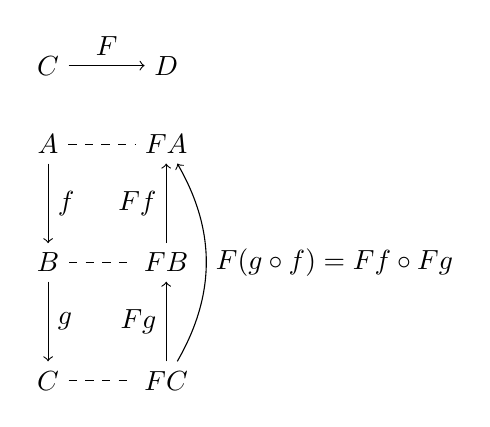
\begin{tikzpicture}[auto]
						\node (a) at (0, 0) {$A$};
						\node (b) at (0, -1.5) {$B$};
						\node (c) at (0, -3) {$C$};
						\node (fa) at (1.5, 0) {$FA$};
						\node (fb) at (1.5, -1.5) {$FB$};
						\node (fc) at (1.5, -3) {$FC$};
						\node (catc) at (0, 1) {$\cat{C}$};
						\node (catd) at (1.5, 1) {$\cat{D}$};
						\draw[-,dashed] (a) to (fa);
						\draw[-,dashed] (b) to (fb);
						\draw[-,dashed] (c) to (fc);
						\draw[->] (a) to node{$f$}(b);
						\draw[->] (b) to node{$g$}(c);
						\draw[->] (fb) to node{$Ff$}(fa);
						\draw[->] (fc) to node{$Fg$}(fb);
						\draw[->,bend right = 30] (fc) to node[swap]{$F(g\circ f)=Ff\circ Fg$}(fa);
						\draw[->] (catc) to node{$F$}(catd);
					\end{tikzpicture}
				\end{center}
				双対圏の射の合成と同じように、合成射を写すときは合成の順序を逆にして写す。
			\end{description}
		\end{quote}
	\end{define}
	反変関手に対して通常の関手を共変関手と呼ぶことにする。
	また反変関手$\functor{F}{C}{D}$は共変関手$\functor{F}{C^{op}}{D}$とみなせる。
		\begin{center}
			\begin{tikzpicture}[auto]
				\node (a) at (0, 0) {$A$};
				\node (b) at (0, -1.5) {$B$};
				\node (fa) at (1.5, 0) {$FA$};
				\node (fb) at (1.5, -1.5) {$FB$};
				\node (catc) at (0, 1) {$\cat{C}$};
				\node (catd) at (1.5, 1) {$\cat{D}$};
				\draw[-,dashed] (a) to (fa);
				\draw[-,dashed] (b) to (fb);
				\draw[->] (a) to node{$f$}(b);
				\draw[->] (fb) to node{$Ff$}(fa);
				\draw[->] (catc) to node{$F$}(catd);

				\node (a) at (3.5, 0) {$A$};
				\node (b) at (3.5, -1.5) {$B$};
				\node (aop) at (5, 0) {$A^{op}$};
				\node (bop) at (5, -1.5) {$B^{op}$};
				\node (fa) at (6.5, 0) {$FA$};
				\node (fb) at (6.5, -1.5) {$FB$};
				\node (catcop) at (3.5, 1) {$\cat{C}$};
				\node (catc) at (5, 1) {$\cat{C^{op}}$};
				\node (catd) at (6.5, 1) {$\cat{D}$};
				\draw[-,dashed] (aop) to (fa);
				\draw[-,dashed] (bop) to (fb);
				\draw[->] (bop) to node{$f^{op}$}(aop);
				\draw[->] (a) to node{$f$}(b);
				\draw[->] (fb) to node{$Ff$}(fa);
				\draw[->] (catc) to node{$F$}(catd);
			\end{tikzpicture}
		\end{center}
	\subsection{Hom関手}
	関手の対、射影関手を定義する際、射集合を集合の圏の対象としてそれらの間の射を考えたが、元の圏に対して集合の圏の射集合やその間の射がどのように関係するかを見ていく。
	\begin{define}[共変射写像]
		圏$\cat{C}$の対象$A,B$と射$\mor{f}{A}{B}$に対して、任意の射$\mor{g}{X}{A}$に射$f$を左から合成する写像を
		\begin{align*}
			&\mor{\arset{C}{X}{f}}{\arset{C}{X}{A}}{\arset{C}{X}{B}}\\
			&\arset{C}{X}{f}(g)=f\circ g
		\end{align*}
		\begin{center}
			\begin{tikzpicture}[auto]
				\node (x) at (-1.5, 0) {$X$};
				\node (x2) at (-1.5, -1.5) {$X$};
				\node (a) at (0, 0) {$A$};
				\node (b) at (0, -1.5) {$B$};
				\node (ca) at (2, 0) {$\arset{C}{X}{A}$};
				\node (cb) at (2, -1.5) {$\arset{C}{X}{B}$};
				\node (catc) at (-0.75, 1) {$\cat{C}$};
				\node (catc) at (2, 1) {$\cat{Set}$};
				\draw[->] (ca) to node{$\arset{C}{X}{f}$}(cb);
				\draw[->] (a) to node{$f$}(b);
				\draw[double distance=2pt] (x) to (x2);
				\draw[->] (x) to node{$g$}(a);
				\draw[->] (x2) to node[swap]{$f\circ g$}(b);
			\end{tikzpicture}
		\end{center}
		と定義する。
	\end{define}
	\begin{prop}[共変射写像の恒等射の保存]
		圏$\cat{C}$の任意の対象$X,A$において
		\[\arset{C}{X}{id_A}=id_{\arset{C}{X}{A}}\]が成り立つ。
		\begin{center}
			\begin{tikzpicture}[auto]
				\node (x) at (-1.5, 0) {$X$};
				\node (x2) at (-1.5, -1.5) {$X$};
				\node (a) at (0, 0) {$A$};
				\node (b) at (0, -1.5) {$A$};
				\node (ca) at (2, 0) {$\arset{C}{X}{A}$};
				\node (cb) at (2, -1.5) {$\arset{C}{X}{A}$};
				\node (catc) at (-0.75, 1) {$\cat{C}$};
				\node (catc) at (2, 1) {$\cat{Set}$};
				\draw[->] (ca) to node{$\arset{C}{X}{id_A}$}(cb);
				\draw[->] (a) to node{$id_A$}(b);
				\draw[double distance=2pt] (x) to (x2);
				\draw[->] (x) to node{$g$}(a);
				\draw[->] (x2) to node[swap]{$g$}(b);
			\end{tikzpicture}
		\end{center}
	\end{prop}
	\begin{proof}
		任意の射$\mor{g}{X}{A}$に対して
		\begin{align*}
			\arset{C}{X}{id_A}(g)&=id_A\circ g&\text{(共変射写像の定義)}\\
			&=g&\text{(単位元律)}\\
			&=id_{\arset{C}{X}{A}}(g)&\text{($\cat{Set}$の恒等射の定義)}\\
		\end{align*}
		よって$\arset{C}{X}{id_A}=id_{\arset{C}{X}{A}}$が成り立つ。
	\end{proof}
	\begin{prop}[共変射写像の合成の保存]
		圏$\cat{C}$の任意の対象$X,A,B,C$と射$\mor{f}{A}{B}$、$\mor{g}{B}{C}$、$\mor{h}{X}{A}$に対して、
		\[\arset{C}{X}{g\circ f}=\arset{C}{X}{g}\circ\arset{C}{X}{f}\]が成り立つ。
		\begin{center}
			\begin{tikzpicture}[auto]
				\node (x) at (-1.5, 0) {$X$};
				\node (x2) at (-1.5, -1.5) {$X$};
				\node (x3) at (-1.5, -3) {$X$};
				\node (a) at (0, 0) {$A$};
				\node (b) at (0, -1.5) {$B$};
				\node (c) at (0, -3) {$C$};
				\node (ca) at (2, 0) {$\arset{C}{X}{A}$};
				\node (cb) at (2, -1.5) {$\arset{C}{X}{B}$};
				\node (cc) at (2, -3) {$\arset{C}{X}{C}$};
				\node (catc) at (-0.75, 1) {$\cat{C}$};
				\node (catc) at (2, 1) {$\cat{Set}$};
				\draw[->] (ca) to node{$\arset{C}{X}{f}$}(cb);
				\draw[->] (cb) to node{$\arset{C}{X}{g}$}(cc);
				\draw[->] (a) to node{$f$}(b);
				\draw[->] (b) to node{$g$}(c);
				\draw[double distance=2pt] (x) to (x2);
				\draw[double distance=2pt] (x2) to (x3);
				\draw[->] (x) to node{$h$}(a);
				\draw[->] (x2) to node[swap]{$f\circ h$}(b);
				\draw[->] (x3) to node[swap]{$g\circ(f\circ h)$}(c);
			\end{tikzpicture}
		\end{center}
	\end{prop}
	\begin{proof}
		任意の射$\mor{h}{X}{A}$に対して
		\begin{align*}
			\arset{C}{X}{g\circ f}(h)&=(g\circ f)\circ h&\text{(共変射関数の定義)}\\
			&=g\circ(f\circ h)&\text{(結合則)}\\
			&=\arset{C}{X}{g}(f\circ h)&\text{(共変射関数の定義)}\\
			&=\arset{C}{X}{g}(\arset{C}{X}{f}(h))&\text{(共変射関数の定義)}\\
			&=\arset{C}{X}{g}\circ\arset{C}{X}{f}(h)&\text{(写像の合成の定義)}\\
		\end{align*}
		よって$\arset{C}{X}{g\circ f}=\arset{C}{X}{g}\circ\arset{C}{X}{f}$が成り立つ。
	\end{proof}
	ここまでの共変射写像の性質から、射から共変射写像を取る操作は関手とみなせることに気が付けたかもしれない。実際にHom関手と呼ばれる関手が定義できる・。
	\begin{define}[共変Hom関手]
		任意の圏$\cat{C}$とそのある対象$X$における共変Hom関手$\functor{\arset{C}{X}{-}}{C}{Set}$を以下の要素で定義する。
		\begin{quote}
			\begin{description}
				\item[対象関数] 圏$\cat{C}$の任意の対象$A$に対して対象関数を
				\begin{align*}
					&\mor{\arset{C}{X}{-}}{\obj{C}}{\obj{Set}}\\
					&\arset{C}{X}{-}(A)=\arset{C}{X}{A}
				\end{align*}
				と定義する。
				\item[射関数] 圏$\cat{C}$の任意の対象$A,B$、射$\mor{f}{A}{B}$に対して射関数を
				\begin{align*}
					&\mor{\arset{C}{X}{-}_{A,B}}{\arset{C}{A}{B}}{\arset{Set}{\arset{C}{X}{A}}{\arset{C}{X}{B}}}\\
					&\arset{C}{X}{-}_{A,B}(f)=\arset{C}{X}{f}
				\end{align*}
				と定義する。
				\begin{center}
					\begin{tikzpicture}[auto]
						\node (a) at (0, 0) {$A$};
						\node (b) at (0, -1.5) {$B$};
						\node (ca) at (2, 0) {$\arset{C}{X}{A}$};
						\node (cb) at (2, -1.5) {$\arset{C}{X}{B}$};
						\node (catc) at (0, 1) {$\cat{C}$};
						\node (catset) at (2, 1) {$\cat{Set}$};
						\draw[->] (ca) to node{$\arset{C}{X}{f}$}(cb);
						\draw[->] (a) to node{$f$}(b);
						\draw[->] (catc) to node{$\arset{C}{X}{-}$}(catset);
						\draw[-,dashed] (a) to (ca);
						\draw[-,dashed] (b) to (cb);
					\end{tikzpicture}
				\end{center}
				\item[恒等射の保存] 共変射写像の合成の保存より、$\arset{C}{X}{id_A}=id_{\arset{C}{X}{A}}$が成り立つ。
				\item[射の合成の保存] 共変射写像の恒等射の保存より、$\arset{C}{X}{g\circ f}=\arset{C}{X}{g}\circ\arset{C}{X}{f}$が成り立つ。
			\end{description}
		\end{quote}
	\end{define}
	共変射写像では射を左から合成する写像を考えたが、次は射を右から合成する写像である反変射写像を考える。
	\begin{define}[反変射写像]
		圏$\cat{C}$の対象$A,B$と射$\mor{f}{A}{B}$に対して、任意の射$\mor{g}{X}{B}$に射$f$を右から合成する写像を
		\begin{align*}
			&\mor{\arset{C}{f}{X}}{\arset{C}{B}{X}}{\arset{C}{A}{X}}\\
			&\arset{C}{f}{X}(g)=g\circ f
		\end{align*}
		\begin{center}
			\begin{tikzpicture}[auto]
				\node (x) at (0, 0) {$X$};
				\node (x2) at (0, -1.5) {$X$};
				\node (a) at (-1.5, 0) {$A$};
				\node (b) at (-1.5, -1.5) {$B$};
				\node (ca) at (2, 0) {$\arset{C}{A}{X}$};
				\node (cb) at (2, -1.5) {$\arset{C}{B}{X}$};
				\node (catc) at (-0.75, 1) {$\cat{C}$};
				\node (catc) at (2, 1) {$\cat{Set}$};
				\draw[->] (cb) to node{$\arset{C}{f}{X}$}(ca);
				\draw[->] (a) to node{$f$}(b);
				\draw[double distance=2pt] (x) to (x2);
				\draw[->] (a) to node{$g\circ f$}(x);
				\draw[->] (b) to node[swap]{$g$}(x2);
			\end{tikzpicture}
		\end{center}
		と定義する。共変射写像と違い、射$f$に対して$\arset{C}{f}{X}$の向きが逆になっている。
	\end{define}
	また反変射写像をとる操作を射関数とした関手は反変関手として定義する。
		\begin{define}[反変Hom関手]
		任意の圏$\cat{C}$とそのある対象$X$における反変Hom関手$\functor{\arset{C}{X}{-}}{C^{op}}{Set}$を以下の要素で定義する。
		\begin{quote}
			\begin{description}
				\item[対象関数] 圏$\cat{C}$の任意の対象$A$に対して対象関数を
				\begin{align*}
					&\mor{\arset{C}{-}{X}}{\obj{C}}{\obj{Set}}\\
					&\arset{C}{-}{X}(A)=\arset{C}{X}{A}
				\end{align*}
				と定義する。
				\item[射関数] 圏$\cat{C}$の任意の対象$A,B$、射$\mor{f}{A}{B}$に対して射関数を
				\begin{align*}
					&\mor{\arset{C}{-}{X}_{A,B}}{\arset{C}{A}{B}}{\arset{Set}{\arset{C}{B}{X}}{\arset{C}{A}{X}}}\\
					&\arset{C}{-}{X}_{A,B}(f)=\arset{C}{f}{X}
				\end{align*}
				と定義する。
				\begin{center}
					\begin{tikzpicture}[auto]
						\node (a) at (0, 0) {$A$};
						\node (b) at (0, -1.5) {$B$};
						\node (ca) at (2, 0) {$\arset{C}{A}{X}$};
						\node (cb) at (2, -1.5) {$\arset{C}{B}{X}$};
						\node (catc) at (0, 1) {$\cat{C}$};
						\node (catset) at (2, 1) {$\cat{Set}$};
						\draw[->] (cb) to node{$\arset{C}{f}{X}$}(ca);
						\draw[->] (a) to node{$f$}(b);
						\draw[->] (catc) to node[swap]{$\arset{C}{-}{X}$}(catset);
						\draw[-,dashed] (a) to (ca);
						\draw[-,dashed] (b) to (cb);
					\end{tikzpicture}
				\end{center}
				\item[恒等射の保存] 共変射写像の合成の保存と同様に$\arset{C}{id_A}{X}=id_{\arset{C}{A}{X}}$が成り立つ。
				\item[射の合成の保存] 共変射写像の恒等射の保存と同様に$\arset{C}{g\circ f}{X}=\arset{C}{f}{X}\circ\arset{C}{g}{X}$が成り立つ。
			\end{description}
		\end{quote}
	\end{define}
	\begin{prop}[Hom関手の積の保存]
		圏$\cat{C}$の積$A\times B$に対して、\[\arset{C}{X}{A\times B}\cong \arset{C}{X}{A}\times \arset{C}{X}{B}\]が成り立つ。
	\end{prop}
	\begin{proof}
		$\arset{C}{X}{A}\times\arset{C}{X}{B}$は$\arset{C}{X}{A}$と$\arset{C}{X}{B}$の積であるが、$\arset{C}{X}{A\times B}$も同様に$\arset{C}{X}{A}$と$\arset{C}{X}{B}$の積であることを示せばよい。
		射影射をそれぞれ
		\begin{align*}
			&\pi_{\arset{C}{X}{A}}=\mor{\arset{C}{X}{\pi_A}}{\arset{C}{X}{A\times B}}{\arset{C}{X}{A}}\\
			&\pi_{\arset{C}{X}{B}}=\mor{\arset{C}{X}{\pi_B}}{\arset{C}{X}{A\times B}}{\arset{C}{X}{B}}
		\end{align*}
		として、組$(\arset{C}{X}{A\times B},\arset{C}{X}{\pi_A},\arset{C}{X}{\pi_B})$が積の普遍性を満たすことを証明する。つまり$\cat{Set}$の任意の対象$Y$と任意の二射$\mor{i}{Y}{\arset{C}{X}{A}}$、$\mor{j}{Y}{\arset{C}{X}{B}}$に対して、
		\begin{align*}
			&\arset{C}{X}{\pi_A}\circ\tuple{i,j}=i\\
			&\arset{C}{X}{\pi_B}\circ\tuple{i,j}=j
		\end{align*}
		が成り立つような射$\mor{\tuple{i,j}}{Y}{\arset{C}{X}{A\times B}}$が一意に存在することを示せばよい。

		まずは図式を可換にする$\tuple{i,j}$が存在することを示す。
		\begin{center}
			\begin{tikzpicture}[auto]
				\node (set) at (3, 3) {$\cat{Set}$};
				\node (xa) at (0, 0) {$\arset{C}{X}{A}$};
				\node (xab) at (3, 0) {$\arset{C}{X}{A\times B}$};
				\node (xb) at (6, 0) {$\arset{C}{X}{B}$};
				\node (y) at (3, 2) {$Y$};
				\draw[->] (xab) to node{$\arset{C}{X}{\pi_A}$}(xa);
				\draw[->] (xab) to node[swap]{$\arset{C}{X}{\pi_B}$}(xb);
				\draw[->] (y) to node[swap]{$i$}(xa);
				\draw[->] (y) to node{$j$}(xb);
				\draw[->] (y) to node{$\tuple{i,j}$}(xab);
			\end{tikzpicture}
		\end{center}
		ここで対象$Y$の任意の元$y$を取り適用すると、圏$\cat{C}$の射$\mor{i(y)}{X}{A}$、$\mor{j(y)}{X}{B}$が得られる。

		射$i,j$は$\cat{Set}$の射であるが、値を適用した$i(y),j(y)$もまた$\cat{C}$の射であることに注意してほしい。もし圏$\cat{C}$で対象$X$の元$x$が取れるなら、さらに値を適用して対象$A$の元$i(y)(x)$が取れる。

		圏$\cat{C}$の積$(A\times B,\pi_A,\pi_B)$に対して射$i(y),j(y)$の射の対\[\mor{\tuple{i(y),j(y)}}{X}{A\times B}\]を考える。
		\begin{center}
			\begin{tikzpicture}[auto]
				\node (a) at (0, 0) {$A$};
				\node (b) at (4, 0) {$B$};
				\node (ab) at (2, 0) {$A\times B$};
				\node (x) at (2, 2) {$X$};
				\draw[->] (ab) to node {$\pi_A$}(a);
				\draw[->] (ab) to node[swap] {$\pi_B$}(b);
				\draw[->] (x) to node[swap] {$i(y)$}(a);
				\draw[->] (x) to node {$j(y)$}(b);
				\draw[->] (x) to node {\scriptsize{$\tuple{i(y),j(y)}$}}(ab);
			\end{tikzpicture}
		\end{center}
		このような射の対は任意の射$i(y),j(y)$に対して存在するから、任意の$y$に対しても存在する。
		よって$\cat{Set}$の射の対$\tuple{i,j}$を任意の$y$に対して\[\tuple{i,j}(y)=\tuple{i(y),j(y)}\]と定義できた。
		次に$\tuple{i,j}$が図式を可換にすることを示す。

		同様に$Y$の任意の元$y$に対し
		\begin{align*}
			\arset{C}{X}{\pi_A}\circ\tuple{i,j}(y)&=\arset{C}{X}{\pi_A}(\tuple{i,j}(y))&\text{(射の合成の定義)}\\
			&=\arset{C}{X}{\pi_A}(\tuple{i(y),j(y)})&\text{($\tuple{i,j}$の定義)}\\
			&=\pi_A\circ(\tuple{i(y),j(y)})&\text{(共変射写像の定義)}\\
			&=i(y)&\text{(射の対の可換性)}
		\end{align*}
		よって$\arset{C}{X}{\pi_A}\circ\tuple{i,j}=i$が成り立つ。同様に$\arset{C}{X}{\pi_B}\circ\tuple{i,j}=j$も成り立つ。

		次に射の対$\tuple{i,j}$の一意性を示す。
		ある射$\mor{k}{Y}{\arset{C}{X}{A\times B}}$が
		\begin{align*}
			&\arset{C}{X}{\pi_A}\circ k=i\\
			&\arset{C}{X}{\pi_B}\circ k=j
		\end{align*}
		を満たすとき、$h=\tuple{i,j}$が成り立つことを示せばよい。

		$Y$の任意の元$y$に対し
		\begin{align*}
			i(y)&=(\arset{C}{X}{\pi_A}\circ k)(y)\\
			&=\arset{C}{X}{\pi_A}(k(y))&\text{(射の合成の定義)}\\
			&=\pi_A\circ(k(y))&\text{(共変射写像の定義)}
		\end{align*}
		よって$\pi_A\circ(k(y))=i(y)$が成り立つ。同様に$\pi_A\circ(k(y))=i(y)$も成り立つ。
		すると$\cat{C}$の積$A\times B$の射の対$\tuple{i,j}(y)$の一意性より、$k(y)=\tuple{i,j}(y)$となる。
		これは任意の$y$で成り立つから$k=\tuple{i,j}$となり、$\tuple{i,j}$は$i,j$に対して一意に存在することが示せた。
		\begin{center}
			\begin{tikzpicture}[auto]
				\node (a) at (0, 0) {$A$};
				\node (b) at (4, 0) {$B$};
				\node (ab) at (2, 0) {$A\times B$};
				\node (x) at (2, 2) {$X$};
				\draw[->] (ab) to node {$\pi_A$}(a);
				\draw[->] (ab) to node[swap] {$\pi_B$}(b);
				\draw[->] (x) to node[swap] {$i(y)$}(a);
				\draw[->] (x) to node {$j(y)$}(b);
				\draw[->,transform canvas={xshift=+2pt}] (x) to node {\scriptsize{$\tuple{i,j}(y)$}}(ab);
				\draw[->,transform canvas={xshift=-2pt}] (x) to node[swap] {\scriptsize{$k(y)$}}(ab);
			\end{tikzpicture}
		\end{center}
		よって組$(\arset{C}{X}{A\times B},\arset{C}{X}{\pi_A},\arset{C}{X}{\pi_B})$は積の普遍性を満たす。つまり$\arset{C}{X}{A\times B}$は$\arset{C}{X}{A}$と$\arset{C}{X}{B}$の積であり、積の一意性より、\[\arset{C}{X}{A\times B}\cong \arset{C}{X}{A}\times \arset{C}{X}{B}\]が成り立つ。
	\end{proof}
	かなり長い証明になってしまったが、$\arset{C}{X}{A\times B}\cong \arset{C}{X}{A}\times \arset{C}{X}{B}$を示すだけなら同型射となるような射を定義して同型射であることを証明すればよい。こちらの方が簡単ではあるが、射集合を用いた議論に慣れてもらうためこのように証明した。

	さてこの同型の意味を考えると、任意の二射$\mor{f}{X}{A}$、$\mor{g}{X}{B}$と射の対$\mor{\tuple{f,g}}{X}{A\times B}$が一対一対応をする、ということになる。つまり積の普遍性で述べた存在と一意性が$\cat{Set}$の同型で述べた存在と一意性で表せることがわかる。

	次に自明ではあるが、共変Hom関手が終対象を保つことを同様に証明する。
	\begin{prop}[Hom関手の終対象の保存]
		圏$\cat{C}$の終対象$1$と圏$\cat{Set}$の任意の対象$X$と終対象$I$に対して\[\arset{C}{X}{1}\cong I\]が成り立つ。
	\end{prop}
	\begin{proof}
		$\arset{C}{X}{1}$が$\cat{Set}$における終対象であることを示せばよい。つまり$\cat{Set}$の任意の対象$Y$に対して\[\mor{!_Y}{Y}{\arset{C}{X}{1}}\]が一意に存在することを証明する。

		射$\mor{!_Y}{Y}{\arset{C}{X}{1}}$が少なくとも一つは存在すると仮定する。
		対象$Y$の任意の元$y$を$!_Y$に適用すると圏$\cat{C}$の射$\mor{!_Y(y)}{X}{1}$が得られるが、終対象$1$の普遍性よりこのような射は少なくとも一つは存在する。よって任意の$y$において$!_Y(y)$が存在するから、実際に射$!_Y$は存在する。
		\begin{center}
			\begin{tikzpicture}[auto]
				\node (set) at (1, 1) {$\cat{Set}$};
				\node (1) at (0, 0) {$Y$};
				\node (1') at (2, 0) {$\arset{C}{X}{1}$};
				\node (set) at (5, 1) {$\cat{C}$};
				\node (x) at (4, 0) {$X$};
				\node (t) at (6, 0) {$1$};
				\draw[->] (1) to node{$!_Y$}(1');
				\draw[->] (x) to node{$!_Y(y)$}(t);
			\end{tikzpicture}
		\end{center}
		次に$\mor{!_Y}{Y}{\arset{C}{X}{1}}$の一意性を示す。つまり射$\mor{h}{Y}{\arset{C}{X}{1}}$が存在したとき、$!_Y=h$が成り立てばよい。

		対象$Y$の任意の元$y$において射$\mor{h(y)}{X}{1}$圏$\cat{C}$の終対象の普遍性より、$\mor{!_Y(y)}{X}{1}$なる射は一意に存在する。よって$!_Y(y)=h(y)$となり、任意の元$y$で成り立つから$!_Y=h$となる。


		\begin{center}
			\begin{tikzpicture}[auto]
				\node (set) at (1, 1) {$\cat{Set}$};
				\node (1) at (0, 0) {$Y$};
				\node (1') at (2, 0) {$\arset{C}{X}{1}$};
				\node (set) at (5, 1) {$\cat{C}$};
				\node (x) at (4, 0) {$X$};
				\node (t) at (6, 0) {$1$};
				\draw[->,transform canvas={yshift=2pt}] (1) to node{$!_Y$}(1');
				\draw[->,transform canvas={yshift=2pt}] (x) to node{$!_Y(y)$}(t);
				\draw[->,transform canvas={yshift=-2pt}] (1) to node[swap]{$h$}(1');
				\draw[->,transform canvas={yshift=-2pt}] (x) to node[swap]{$h(y)$}(t);
			\end{tikzpicture}
		\end{center}
		$\mor{!_Y}{Y}{\arset{C}{X}{1}}$なる射が一意に存在することが示せたから、$\arset{C}{X}{1}$は$\cat{Set}$における終対象となる。よって終対象の一意性より、\[\arset{C}{X}{1}\cong I\]が成り立つ。
	\end{proof}
	共変Hom関手、反変Hom関手を双関手として定義する。
	\begin{define}[双Hom関手]
		任意の圏$\cat{C}$における双Hom関手$\functor{C(-,-)}{C^{op}\times C}{Set}$を以下の要素で定義する。
		\begin{quote}
			\begin{description}
				\item[対象関数] 積圏$\cat{C^{op}\times C}$の任意の対象$[A,B]$に対して対象関数を
				\begin{align*}
					&\mor{\arset{C}{-}{-}}{\obj{C^{op}\times C}}{\obj{Set}}\\
					&\arset{C}{-}{-}([A,B])=\arset{C}{A}{B}
				\end{align*}
				と定義する。
				\item[射関数] 射関数を定義する前に共変射写像、反変射写像の双Hom関手版を定義する。
				圏$\cat{C^{op}}$の任意の射$\mor{f^{op}}{A^{op}}{A'^{op}}$、つまり圏$\cat{C}$の射$\mor{f}{A'}{A}$と圏$\cat{C}$の任意の射$\mor{g}{B}{B'}$に対し射写像\[\mor{\arset{C}{f}{g}}{\arset{C}{A}{B}}{\arset{C}{A'}{B'}}\]を任意の射$\mor{h}{A}{B}$において、
				\begin{align*}
					\arset{C}{f}{g}&=\arset{C}{f}{B'}\circ\arset{C}{A}{g}\\
					&=\arset{C}{A'}{g}\circ\arset{C}{f}{B}\\
					\arset{C}{f}{g}(h)&=g\circ h\circ f\\
				\end{align*}
				と定義する。

				\begin{center}
					\begin{tikzpicture}[auto]
						\node (A) at (0, 0) {$A$};
						\node (A') at (0, -2) {$A'$};
						\node (B) at (2, 0) {$B$};
						\node (B') at (2, -2) {$B'$};
						\draw[->] (A') to node{$f$}(A);
						\draw[->] (B) to node{$g$}(B');
						\draw[->] (A) to node{$h$}(B);
						\draw[->] (A') to node{$g\circ h\circ f$}(B');
						\node (AB) at (4, 0) {$\arset{C}{A}{B}$};
						\node (A'B') at (4, -2) {$\arset{C}{A'}{B'}$};
						\draw[->] (AB) to node{$\arset{C}{f}{g}$}(A'B');
						\node (catc) at (1, 1) {$\cat{C}$};
						\node (catset) at (4, 1) {$\cat{Set}$};
					\end{tikzpicture}
				\end{center}

				圏$\cat{C^{op}\times C}$の任意の対象$[A,B],[A',B']$、射$\mor{f}{A}{B}$に対して射関数を
				\begin{align*}
					&\mor{\arset{C}{-}{-}}{\arset{(C^{op}\times C)}{[A,B]}{[A',B']}}{\arset{Set}{\arset{C}{A}{B}}{\arset{C}{A'}{B'}}}\\
					&\arset{C}{-}{-}([f,g])=\arset{C}{f}{g}
				\end{align*}
				と定義する。
				\begin{center}
					\begin{tikzpicture}[auto]
						\node (ab) at (0, 0) {$[A,B]$};
						\node (a'b') at (0, -2) {$[A',B']$};
						\draw[->] (ab) to node{$[f,g]$}(a'b');
						\node (sab) at (2, 0) {$\arset{C}{A}{B}$};
						\node (sa'b') at (2, -2) {$\arset{C}{A'}{B'}$};
						\draw[->] (sab) to node{$\arset{C}{f}{g}$}(sa'b');
						\draw[-,dashed] (ab) to (sab);
						\draw[-,dashed] (a'b') to (sa'b');
						\node (catc) at (0, 1) {$\cat{C}$};
						\node (catset) at (2, 1) {$\cat{Set}$};
						\draw[->] (catc) to node{$\arset{C}{-}{-}$}(catset);
					\end{tikzpicture}
				\end{center}
				\item[恒等射の保存] 圏$\cat{C^{op}\times C}$の任意の対象$[A,B]$に対して\[\arset{C}{-}{-}(id_{[A,B]})=\mor{id_{\arset{C}{-}{-}([A,B])}}{\arset{C}{A}{B}}{\arset{C}{A}{B}}\]を示せばよい。

				任意の積圏の射$\mor{f}{A}{B}$に対して
				\begin{align*}
					\arset{C}{-}{-}(id_{[A,B]})(f)&=\arset{C}{-}{-}([id_A,id_B])(f)&\text{(積圏の恒等射の定義)}\\
					&=\arset{C}{id_A}{id_B}(f)&\text{(対象関数の定義)}\\
					&=id_B\circ f\circ id_A&\text{(射写像の定義)}\\
					&=f&\text{(圏$\cat{C}$の単位元律)}\\
					&=id_{\arset{C}{A}{B}}(f)&\text{($\cat{Set}$の単位元律)}\\
					&=id_{\arset{C}{-}{-}([A,B])}(f)&\text{(対象関数の定義)}
				\end{align*}
				よって$\arset{C}{-}{-}(id_{[A,B]})=id_{\arset{C}{-}{-}([A,B])}$が成り立ち恒等射の保存が成り立つ。


				\item[射の合成の保存] $\cat{Set}$の任意の射写像$\mor{\arset{C}{f}{g}}{\arset{C}{A}{B}}{\arset{C}{A'}{B'}}$、$\mor{\arset{C}{f'}{g'}}{\arset{C}{A'}{B'}}{\arset{C}{A''}{B''}}$に対して\[\arset{C}{f'}{g'}\circ\arset{C}{f}{g}=\arset{C}{f\circ f'}{g'\circ g}\]が成り立てばよい。

				圏$\cat{C}$の任意の射$\mor{h}{A}{B}$に対して
				\begin{align*}
					(\arset{C}{f'}{g'}\circ\arset{C}{f}{g})(h)&=(\arset{C}{f'}{g'})(g\circ h\circ f)&\text{(射写像の定義)}\\
					&=g'\circ(g\circ h\circ f)\circ f'&\text{(射写像の定義)}\\
					&=(g'\circ g)\circ h\circ(f\circ f')&\text{(結合律)}\\
					&=\arset{C}{f\circ f'}{g'\circ g}(h)&\text{(射写像の定義)}\\
				\end{align*}
				よって$\arset{C}{f'}{g'}\circ\arset{C}{f}{g}=\arset{C}{f\circ f'}{g'\circ g}$となり射の合成の保存が成り立つ。
			\end{description}
		\end{quote}
	\end{define}

	実は左側の積関手と右側の積関手から双積関手、共変Hom関手と反変Hom関手から双Hom関手を定義できる。またこの定義を用いれば双関手の恒等射の保存と合成の保存を個別に証明しなくても済む。
	\begin{define}[二つの関手による双関手の定義]
		圏$\cat{B}$の任意の対象$B$に対して定義される関手$\functor{F_B}{A}{C}$と、圏$\cat{A}$の任意の対象$A$に対して定義される関手$\functor{G_A}{B}{C}$が存在し、任意の二対象$A,B$に対して\[{F_B}A={G_A}B\]が成り立ち、	任意の二射$\mor{f}{A}{A'}$、$\mor{g}{B}{B'}$に対して\[{G_{A'}}g\circ {F_B}f = {F_{B'}}f\circ {G_A}g\]が成り立つとする。
		\begin{center}
			\begin{tikzpicture}[auto]
				\node (A) at (0, 0.75) {$A$};
				\node (B) at (1.5, 0.75) {$A'$};
				\node (FA) at (3, 1.5) {${F_B}A$};
				\node (FB) at (4.5, 1.5) {${F_B}A'$};
				\node (GA) at (3, 0) {${F_{B'}}A$};
				\node (GB) at (4.5, 0) {${F_{B'}}A'$};

				\node (catc) at (0.75, 3) {$\cat{A}$};
				\node (catd) at (3.75, 3) {$\cat{C}$};

				\draw[->] (A) to node{$f$}(B);
				\draw[->] (FA) to node{${F_B}f$}(FB);
				\draw[->] (GA) to node{${F_{B'}}f$}(GB);
				\draw[->,bend left = 20] (catc) to node (funcf){$F_B$}(catd);
				\draw[->,bend right = 20] (catc) to node (funcg)[swap]{$F_{B'}$}(catd);
			\end{tikzpicture}
			\begin{tikzpicture}[auto]
				\node (A) at (0.75, 0) {$B$};
				\node (B) at (0.75, 1.5) {$B'$};
				\node (FA) at (3, 1.5) {${G_A}B$};
				\node (FB) at (4.5, 1.5) {${G_{A'}}B$};
				\node (GA) at (3, 0) {${G_{A}}B'$};
				\node (GB) at (4.5, 0) {${G_{A'}}B'$};

				\node (catc) at (0.75, 3) {$\cat{B}$};
				\node (catd) at (3.75, 3) {$\cat{C}$};

				\draw[->] (B) to node{$g$}(A);
				\draw[->] (FA) to node{${G_A}g$}(GA);
				\draw[->] (FB) to node{${G_{A'}}g$}(GB);

				\draw[->,bend left = 20] (catc) to node (funcf){$G_A$}(catd);
				\draw[->,bend right = 20] (catc) to node (funcg)[swap]{$G_{A'}$}(catd);
			\end{tikzpicture}
		\end{center}


		この時、双関手$\functor{H}{A\times B}{C}$を
		\begin{quote}
			\begin{description}
				\item[対象関数] 対象関数\[\mor{H}{\obj{A\times B}}{\obj{C}}\]を積圏の任意の対象$\pcobj{A,B}$に対して
				\[H(A,B)={F_B}A={G_A}B\]と定義する。
				\item[射関数] 射関数\[\mor{H_{\pcobj{A,A'},\pcobj{B,B'}}}{\arset{A\times B}{\pcobj{A,B}}{\pcobj{A',B'}}}{\arset{C}{H(A,B)}{H(A',B')}}\]を積圏の任意の射\[\mor{\pcobj{f,g}}{\pcobj{A,B}}{\pcobj{A',B'}}\]に対して、\[H_{\pcobj{A,A'},\pcobj{B,B'}}(\pcobj{f,g})={G_{A'}}g\circ {F_B}f = {F_{B'}}f\circ {G_A}g\]と定義する。
				\item[恒等射の保存]$H(id_{\pcobj{A,B}})=id_{H(A,B)}$を示せばよい。
				\begin{align*}
					H(id_{\pcobj{A,B}})&=H(id_A,id_B)&\text{(積圏の恒等射の定義)}\\
					&=G_A(id_B)\circ F_B(id_A)&\text{(双関手の射関数)}\\
					&=id_{H(A,B)}\circ id_{H(A,B)}&\text{(関手の恒等射の保存)}\\
					&=id_{H(A,B)}&\text{(積圏の単位減律)}
				\end{align*}
				よって恒等射を保存する。
				\item[射の合成の保存]$H(f',g')\circ H(f,g)=H(f'\circ f,g'\circ g)$を示せばよい。
				\begin{align*}
					H(f',g')\circ H(f,g)&=(G_{A''}g'\circ F_{B'}f')\circ(G_{A'}\circ F_Bf)&\text{(射関数の定義)}\\
					&=G_{A''}g'\circ (F_{B'}f'\circ G_{A'})\circ  F_Bf&\text{(積圏の結合律)}\\
					&=G_{A''}g'\circ G_{A''}g\circ F_Bf'\circ  F_Bf&\text{(射関数の定義)}\\
					&=(G_{A''}g'\circ G_{A''}g)\circ (F_Bf'\circ  F_Bf)&\text{(積圏の結合則)}\\
					&=G_{A''}(g'\circ g)\circ F_B(f'\circ f)&\text{($G_{A''}$と$F_B$の合成の保存)}\\
					&=H(f'\circ f,g'\circ g)&\text{(射関数の定義)}\\
				\end{align*}
			\end{description}
		\end{quote}
		証明が少し複雑になってしまったが、何とか証明できた。
	\end{define}
	次に例として二つの積関手から双積関手を定義する。

	$\cat{C}$の任意の対象$A,B$に対する積関手$\functor{(A\times -)}{C}{C}$と$\functor{(-\times B)}{C}{C}$から双関手$\functor{(-\times -)}{C\times C}{C}$を構成する。
	まず\[(A\times -)(B)=(-\times B)(A)\]と、任意の射$\mor{f}{A}{A'}$、$\mor{g}{B}{B'}$において
	\[(A'\times -)g\circ (-\times B)f=(-\times B')f\circ(A\times -)g\]が成り立つから、確かに双積関手を構成するための条件は満たしている。

	ここで双積関手$\functor{(-\times -)}{C\times C}{C}$の対象関数を積圏の任意の対象$\pcobj{A,B}$に対して
	\begin{align*}
		\mor{&(-\times -)}{\obj{C\times C}}{\obj{C}}\\
		&(-\times -)(\pcobj{A,B})=(A\times -)(B)=(-\times B)(A)
	\end{align*}
	とする。
	同様に射関数を積圏の任意の射$\mor{\pcobj{f,g}}{\pcobj{A,B}}{\pcobj{A,B}}$に対して
	\begin{align*}
		\mor{&(-\times -)}{\arset{C\times C}{\pcobj{A,B}}{\pcobj{A',B'}}}{\arset{C}{A\times B}{A'\times B'}}\\
		&(-\times -)(\pcobj{f,g})=(A'\times -)g\circ (-\times B)f=(-\times B')f=(A\times -)g
	\end{align*}
	とする。

	すると二つの関手による双関手の定義から、このように定義した双積関手は恒等射と射の合成を保つ。よって実際に関手になる。

	また対象関数と射関数は
	\begin{align*}
		(-\times -)(\pcobj{A,B})&=(A\times -)(B)&\text{(対象関数の定義)}\\
		&=A\times B&\text{(積関手の対象関数の定義)}\\
		(-\times -)(\pcobj{f,g})&=(A'\times -)g\circ (-\times B)f&\text{射関数の定義}\\
		&=(id_{A'}\times g)\circ(f\times id_B)&\text{(積関手の射関数の定義)}\\
		&=f\times g&\text{(積と合成の交換)}
	\end{align*}
	となるから、今定義した双積関手と元の対応から直接定義した双積関手は等しいことが分かる。


	\section{自然変換}
	次に関手の間の射である自然変換を定義する。
	\begin{define}
		二つの関手$\functor{F,G}{C}{D}$の間の自然変換$\natf{\alpha}{F}{G}{C}{D}$は以下で定義される成分と呼ばれる射で構成される。
		\begin{quote}
			\begin{description}
				\item[成分] 圏$\cat{C}$の任意の対象$X$に対する自然変換$\alpha$の成分$\alpha_X$とは\[\mor{\alpha_X}{FX}{GX}\]となるような射である。つまりこの成分をすべての対象の分だけ集めたものが自然変換である。
				\item[自然性]
				自然変換とその成分は以下の自然性を満たさなければならない。

				圏$\cat{C}$の任意の射$\mor{f}{A}{B}$を関手$F,G$で写した射$\mor{Ff}{FA}{FB}$、$\mor{Gf}{GA}{GB}$に対して、\[Gf\circ\alpha_A=\alpha_B\circ Ff\]が成り立つことを自然性と呼ぶ。
				\begin{center}
					\begin{tikzpicture}[auto]
						\node (A) at (0, 0.75) {$A$};
						\node (B) at (1.5, 0.75) {$B$};
						\node (FA) at (3, 1.5) {$FA$};
						\node (FB) at (4.5, 1.5) {$FB$};
						\node (GA) at (3, 0) {$GA$};
						\node (GB) at (4.5, 0) {$GB$};

						\node (catc) at (0.75, 3) {$\cat{C}$};
						\node (catd) at (3.75, 3) {$\cat{D}$};

						\draw[->] (A) to node{$f$}(B);
						\draw[->] (FA) to node{$Ff$}(FB);
						\draw[->] (GA) to node{$Gf$}(GB);
						\draw[->] (FA) to node{$\alpha_A$}(GA);
						\draw[->] (FB) to node{$\alpha_B$}(GB);

						\draw[->,bend left = 30] (catc) to node (funcf){$F$}(catd);
						\draw[->,bend right = 30] (catc) to node (funcg)[swap]{$G$}(catd);
						\draw[double,double equal sign distance,-implies,shorten >=5pt,shorten <=5pt] (funcf) -- node[label=right:$\alpha$] {} (funcg);
					\end{tikzpicture}
				\end{center}
				つまり自然変換は関手$F,G$で写された対象同士に成分で橋を架け、自然性を用いて橋と橋の間に肉付けを行うイメージである。
			\end{description}
		\end{quote}
		次に具体的な自然変換の例を紹介する。
	\end{define}
	圏$\cat{C,D}$を以下の対象、射で構成される。また$l\circ k=j\circ i$とする。
	\begin{center}
		\begin{tikzpicture}[auto]
			\node (a) at (0, 2) {$A$};
			\node (b) at (0, 0) {$B$};
			\node (c) at (2, 1) {$C$};
			\draw[->] (a) to node{$f$}(b);
			\draw[->] (b) to node{$g$}(c);
			\draw[->] (a) to node{$g\circ f$}(c);

			\node (x) at (4, 2) {$X$};
			\node (y) at (4, 0) {$Y$};
			\node (w) at (6, 2) {$W$};
			\node (z) at (6, 0) {$Z$};
			\draw[->] (x) to node{$i$}(y);
			\draw[->] (y) to node{$j$}(z);
			\draw[->] (x) to node{$j\circ i$}(z);
			\draw[->] (w) to node{$l$}(z);
			\draw[->,transform canvas={yshift=-2pt}] (x) to node[swap]{$k$}(w);
			\draw[->,transform canvas={yshift=2pt}] (x) to node{$k\circ h$}(w);
			\draw[->,loop left ,looseness=10] (x) to node{$h$}(x);

			\node (catc) at (1, 3) {$\cat{C}$};
			\node (catd) at (5, 3) {$\cat{D}$};
		\end{tikzpicture}
	\end{center}
	関手$\functor{S,T}{C}{D}$を以下の対象と射の対応によって定義される関手とする。
	\begin{center}
		\begin{tikzpicture}[auto]
			\node (ta) at (4, 2) {$SA$};
			\node (tb) at (4, 0) {$SB$};
			\node (tc) at (6, 1) {$SC$};
			\node (x) at (8, 2) {$X$};
			\node (y) at (8, 0) {$X$};
			\node (z) at (10, 1) {$W$};

			\node (e) at (7, 1) {$=$};

			\draw[-, line width=4pt,draw=white] (x) to (y);
			\draw[->] (x) to node[yshift =10]{$h$}(y);
			\draw[->] (y) to node[swap]{$k$}(z);
			\draw[->] (x) to node{$k\circ h$}(z);

			\draw[-, line width=4pt,draw=white] (ta) to (tb);
			\draw[->] (ta) to node[yshift =10]{$Sf$}(tb);
			\draw[->] (tb) to node[swap]{$Sg$}(tc);
			\draw[->] (ta) to node{$S(g\circ f)$}(tc);

			\node (catd) at (7, 3) {$\cat{D}$};
		\end{tikzpicture}
	\end{center}
	\begin{center}
		\begin{tikzpicture}[auto]
			\node (ta) at (4, 2) {$TA$};
			\node (tb) at (4, 0) {$TB$};
			\node (tc) at (6, 1) {$TC$};
			\node (x) at (8, 2) {$X$};
			\node (y) at (8, 0) {$Y$};
			\node (z) at (10, 1) {$Z$};

			\node (e) at (7, 1) {$=$};

			\draw[-, line width=4pt,draw=white] (x) to (y);
			\draw[->] (x) to node[yshift =10]{$i$}(y);
			\draw[->] (y) to node[swap]{$j$}(z);
			\draw[->] (x) to node{$j\circ i$}(z);

			\draw[-, line width=4pt,draw=white] (ta) to (tb);
			\draw[->] (ta) to node[yshift =10]{$Tf$}(tb);
			\draw[->] (tb) to node[swap]{$Tg$}(tc);
			\draw[->] (ta) to node{$T(g\circ f)$}(tc);

			\node (catd) at (7, 3) {$\cat{D}$};
		\end{tikzpicture}
	\end{center}
	関手$S,T$の間の自然変換$\natf{\alpha}{S}{T}{C}{D}$を以下の成分で定義する。
	\begin{align*}
		\mor{\alpha_A}{SA}{TA}&=\mor{h}{X}{X}\\
		\mor{\alpha_B}{SB}{TB}&=\mor{i}{X}{Y}\\
		\mor{\alpha_C}{SC}{TC}&=\mor{l}{W}{Z}
	\end{align*}
	\begin{center}
		\begin{tikzpicture}[auto]
			\node (sa) at (0, 2) {$SA$};
			\node (sb) at (2, 2) {$SB$};
			\node (sc) at (4, 2) {$SC$};
			\node (ta) at (0, 0) {$TA$};
			\node (tb) at (2, 0) {$TB$};
			\node (tc) at (4, 0) {$TC$};
			\node (e) at (5, 1) {$=$};
			\draw[->] (sa) to node{$Sf$}(sb);
			\draw[->] (sb) to node{$Sg$}(sc);
			\draw[->] (ta) to node{$Tf$}(tb);
			\draw[->] (tb) to node{$Tg$}(tc);
			\draw[->] (sa) to node{$\alpha_A$}(ta);
			\draw[->] (sb) to node{$\alpha_B$}(tb);
			\draw[->] (sc) to node{$\alpha_C$}(tc);

			\node (sa') at (6, 2) {$X$};
			\node (sb') at (8, 2) {$X$};
			\node (sc') at (10, 2) {$W$};
			\node (ta') at (6, 0) {$X$};
			\node (tb') at (8, 0) {$Y$};
			\node (tc') at (10, 0) {$Z$};
			\draw[->] (sa') to node{$h$}(sb');
			\draw[->] (sb') to node{$k$}(sc');
			\draw[->] (ta') to node{$i$}(tb');
			\draw[->] (tb') to node{$j$}(tc');
			\draw[->] (sa') to node{$h$}(ta');
			\draw[->] (sb') to node{$i$}(tb');
			\draw[->] (sc') to node{$l$}(tc');
		\end{tikzpicture}
	\end{center}
	すると、
	\begin{align*}
		\alpha_B\circ Sf&=i\circ h\\
		&=Tf\circ\alpha_A\\
		\alpha_C\circ Sg&=l\circ k\\
		&=j\circ i\\
		&=Tg\circ\alpha_B
	\end{align*}
	となり、このような成分の定義は自然性を満たす。
	よって確かに$\alpha$は自然変換となる。

	次に自然変換の例を示す。

	ある圏$\cat{C}$の任意の対象$X$の恒等射$\mor{id_X}{X}{X}$はすべての対象に存在するため自然変換の成分$id$とみなせるかもしれない。
	実際に圏$\cat{C}$の二つの恒等関手$\functor{Id_C}{C}{C}$の間の自然変換\[\natf{id}{Id_C}{Id_C}{C}{C}\]を考えると、対象$X$に対する成分は$\mor{id}{Id(X)}{Id(X)}=\mor{id}{X}{X}$となる。
	また任意の射$\mor{f}{A}{B}$において\[id_B\circ f=f\circ id_A\]が成り立つから、確かに自然性を満たす。
	\begin{center}
		\begin{tikzpicture}[auto]
			\node (A) at (0, 1) {$A$};
			\node (B) at (2, 1) {$B$};
			\node (FA) at (4, 2) {$Id(A)$};
			\node (FB) at (6, 2) {$Id(B)$};
			\node (GA) at (4, 0) {$Id(A)$};
			\node (GB) at (6, 0) {$Id(B)$};

			\node (e) at (7.5, 1) {$=$};

			\node (catc) at (1, 4) {$\cat{C}$};
			\node (catd) at (5, 4) {$\cat{D}$};

			\draw[->] (A) to node{$f$}(B);
			\draw[->] (FA) to node{$Id(f)$}(FB);
			\draw[->] (GA) to node{$Id(f)$}(GB);
			\draw[->] (FA) to node{$id_A$}(GA);
			\draw[->] (FB) to node{$id_B$}(GB);

			\node (FA) at (8.5, 2) {$A$};
			\node (FB) at (10.5, 2) {$B$};
			\node (GA) at (8.5, 0) {$A$};
			\node (GB) at (10.5, 0) {$B$};
			\draw[->] (FA) to node{$id_A$}(GA);
			\draw[->] (FB) to node{$id_B$}(GB);
			\draw[->] (FA) to node{$f$}(FB);
			\draw[->] (GA) to node{$f$}(GB);
			\draw[->,bend left = 20] (catc) to node (funcf){$Id_C$}(catd);
			\draw[->,bend right = 20] (catc) to node (funcg)[swap]{$Id_C$}(catd);
			\draw[double,double equal sign distance,-implies,shorten >=5pt,shorten <=5pt] (funcf) -- node[label=right:$id$] {} (funcg);
		\end{tikzpicture}
	\end{center}
	となり、確かに恒等射を成分とする自然変換$id$は自然性を満たす。

	次に自然変換$\natf{id}{Id_C}{Id_C}{C}{C}$を恒等関手$\functor{Id_C}{C}{C}$だけでなく、任意の関手$\functor{F}{C}{D}$で考えられるように一般化する。
	\begin{define}[恒等自然変換]
		関手$\functor{F}{C}{D}$に対して恒等自然変換$\natf{ID_F}{F}{F}{C}{D}$を、圏$C$の任意の対象$X$において\[(ID_F)_{X}=id_{FX}\]と定義する。

		これは\[(ID_F)_B\circ Ff=Ff\circ(ID_F)_A\]より自然性を満たす。
		\begin{center}
			\begin{tikzpicture}[auto]
				\node (A) at (0, 0.75) {$A$};
				\node (B) at (1.5, 0.75) {$B$};
				\node (FA) at (3, 1.5) {$FA$};
				\node (FB) at (4.5, 1.5) {$FB$};
				\node (GA) at (3, 0) {$FA$};
				\node (GB) at (4.5, 0) {$FB$};

				\node (catc) at (0.75, 3) {$\cat{C}$};
				\node (catd) at (3.75, 3) {$\cat{D}$};

				\draw[->] (A) to node{$f$}(B);
				\draw[->] (FA) to node{$Ff$}(FB);
				\draw[->] (GA) to node{$Ff$}(GB);
				\draw[->] (FA) to node[swap]{\scriptsize{$(ID_F)_A$}}(GA);
				\draw[->] (FB) to node{\scriptsize{$(ID_F)_B$}}(GB);

				\draw[->,bend left = 30] (catc) to node (funcf){$F$}(catd);
				\draw[->,bend right = 30] (catc) to node (funcg)[swap]{$F$}(catd);
				\draw[double,double equal sign distance,-implies,shorten >=5pt,shorten <=5pt] (funcf) -- node[label=right:$ID_F$] {} (funcg);
			\end{tikzpicture}
		\end{center}
	\end{define}
	\begin{define}[自然変換の垂直合成]
		任意の関手$\functor{F,G,H}{C}{D}$の間の任意の自然変換$\nat{\alpha}{F}{G}$、$\nat{\beta}{G}{H}$の合成自然変換$\nat{\beta\cdot\alpha}{F}{H}$を、圏$\cat{C}$の任意の対象$X$における成分\[(\beta\cdot\alpha)_X=\mor{\beta_X\circ\alpha_X}{FX}{HX}\]によって定義する。
		\begin{center}
			\begin{tikzpicture}[auto]
				\node (A) at (0, 0) {$A$};
				\node (B) at (1.5, 0) {$B$};
				\node (FA) at (3, 1.5) {$FA$};
				\node (FB) at (4.5, 1.5) {$FB$};
				\node (GA) at (3, 0) {$GA$};
				\node (GB) at (4.5, 0) {$GB$};
				\node (HA) at (3, -1.5) {$HA$};
				\node (HB) at (4.5, -1.5) {$HB$};
				\node (catc) at (0.75, 3) {$\cat{C}$};
				\node (catd) at (3.75, 3) {$\cat{D}$};

				\draw[->] (A) to node{$f$}(B);
				\draw[->] (FA) to node{$Ff$}(FB);
				\draw[->] (GA) to node{$Gf$}(GB);
				\draw[->] (HA) to node{$Hf$}(HB);
				\draw[->] (FA) to node{$\alpha_A$}(GA);
				\draw[->] (FB) to node{$\alpha_B$}(GB);
				\draw[->] (GA) to node{$\beta_A$}(HA);
				\draw[->] (GB) to node{$\beta_B$}(HB);
				\draw[->,bend left = 50] (catc) to node (funcf){$F$}(catd);
				\draw[->] (catc) to node[yshift =-7,fill=white] (funcg){$G$}(catd);
				\draw[->,bend right = 50] (catc) to node (funch)[swap]{$H$}(catd);
				\draw[double,double equal sign distance,-implies,shorten >=2pt,shorten <=3pt] (funcf) -- node[label=right:$\alpha$] {} (funcg);
				\draw[double,double equal sign distance,-implies,shorten >=3pt,shorten <=2pt] (funcg) -- node[label=right:$\beta$] {} (funch);
			\end{tikzpicture}
			\begin{tikzpicture}[auto]
				\node (A) at (0, 0) {$A$};
				\node (B) at (1.5, 0) {$B$};
				\node (FA) at (3, 1.5) {$FA$};
				\node (FB) at (4.5, 1.5) {$FB$};
				\node (HA) at (3, -1.5) {$HA$};
				\node (HB) at (4.5, -1.5) {$HB$};
				\node (catc) at (0.75, 3) {$\cat{C}$};
				\node (catd) at (3.75, 3) {$\cat{D}$};

				\draw[->] (A) to node{$f$}(B);
				\draw[->] (FA) to node{$Ff$}(FB);
				\draw[->] (HA) to node{$Hf$}(HB);
				\draw[->] (FA) to node{$\beta_A\circ\alpha_A$}(HA);
				\draw[->] (FB) to node{$\beta_B\circ\alpha_B$}(HB);
				\draw[->,bend left = 50] (catc) to node (funcf){$F$}(catd);
				\draw[->,bend right = 50] (catc) to node (funch)[swap]{$H$}(catd);
				\draw[double,double equal sign distance,-implies,shorten >=5pt,shorten <=5pt] (funcf) -- node[label=right:$\alpha\cdot\beta$] {} (funch);
			\end{tikzpicture}
		\end{center}
		すると任意の射$\mor{f}{A}{B}$において
		\begin{align*}
			(\beta\cdot\alpha)_B\circ Ff&=\beta_B\circ\alpha_B\circ Ff&\text{(合成自然変換の成分)}\\
			&=\beta_B\circ Gf\circ \alpha_A&\text{($\alpha$の自然性)}\\
			&=Hf\circ\beta_A\circ\alpha_A&\text{($\beta$の自然性)}\\
			&=Hf\circ(\beta\cdot\alpha)_A&\text{(合成自然変換の成分)}
		\end{align*}
		となり、$\beta\cdot\alpha$は確かに自然性を満たす。
	\end{define}
	\begin{prop}[射影射の自然性]
		積を持つ圏$\cat{C}$の任意の積$A\times B$の射影射$\mor{\pi_{LA}}{A\times B}{A}$は、双積関手$\functor{(-\times -)}{C\times C}{C}$から射影関手$\functor{\Pi_{LC}}{C\times C}{C}$への自然変換の成分である。

		この自然変換を\[\nat{\pi_L}{(-\times -)}{\Pi_{LC}}\]とし、成分を\[(\pi_L)_{A\times B}=\mor{\pi_{LA}}{A\times B}{A}\]とする。
		すると、射の積の定義$f\times g = \tuple{f\circ\pi_{LA},g\circ\pi_{RB}}$より、
		\begin{align*}
			(\pi_L)_{A'\times B'}\circ (f\times g)&=\pi_{LA}\circ (f\times g)&\text{(成分の定義)}\\
			&=\pi_{LA}\circ\tuple{f\circ\pi_{LA},g\circ\pi_{RB}}&\text{(射の積の定義)}\\
			&=f\circ\pi_{LA}&\text{(射の対の可換性)}\\
			&=f\circ(\pi_L)_{A\times B}&\text{(成分の定義)}
		\end{align*}
		となり、確かに自然性を満たす。
		\begin{center}
			\begin{tikzpicture}[auto]
				\node (ab) at (0, 1) {$\pcobj{A,B}$};
				\node (a'b') at (2, 1) {$\pcobj{A',B'}$};
				\draw[->] (ab) to node{$\pcobj{f,g}$}(a'b');

				\node (pab) at (4, 2) {$A\times B$};
				\node (pa'b') at (6, 2) {$A'\times B'$};
				\node (a) at (4, 0) {$A$};
				\node (a') at (6, 0) {$A'$};
				\draw[->] (pab) to node{$f\times g$}(pa'b');
				\draw[->] (a) to node{$f$}(a');
				\draw[->] (pab) to node{$(\pi_L)_{A\times B}$}(a);
				\draw[->] (pa'b') to node{$(\pi_L)_{A'\times B'}$}(a');

				\node (catcc) at (1, 3.5) {$\cat{C\times C}$};
				\node (catc) at (5, 3.5) {$\cat{C}$};

				\draw[->,bend left = 20] (catcc) to node (funcf){$(-\times -)$}(catc);
				\draw[->,bend right = 20] (catcc) to node (funch)[swap]{$\Pi_{LC}$}(catc);
				\draw[double,double equal sign distance,-implies,shorten >=5pt,shorten <=5pt] (funcf) -- node[label=right:$\pi_L$] {} (funch);
			\end{tikzpicture}
		\end{center}
	\end{prop}
	\begin{define}[自然変換の水平合成]
		自然変換$\natf{\alpha}{F}{G}{C}{D}$に対して、関手$\functor{F'}{D}{E}$と水平合成した自然変換\[\natf{F'\circ\alpha}{F'F}{F'G}{C}{E}\]を圏$\cat{C}$の任意の対象$X$に対する成分\[(F'\circ\alpha)_X=F'(\alpha_X)\]として定義する。また関手の合成と同様に紛らわしくない場合は$F'\circ\alpha=F'\alpha$と略記する。

		圏$\cat{C}$の任意の射$\mor{f}{A}{B}$とそれによる圏$\cat{D}$の自然変換の図式があるが、この図式を関手$\functor{F'}{D}{E}$で圏$\cat{E}$に写す。この時、$F'$によって写された自然変換の成分が圏$\cat{E}$の自然変換の成分になることを示せばよい。
		\begin{center}
			\begin{tikzpicture}[auto]
				\node (a) at (0, 1) {$A$};
				\node (b) at (2, 1) {$B$};
				\draw[->] (a) to node{$f$}(b);

				\node (fa) at (4, 2) {$FA$};
				\node (fb) at (6, 2) {$FB$};
				\node (ga) at (4, 0) {$GA$};
				\node (gb) at (6, 0) {$GB$};
				\draw[->] (fa) to node{$Ff$}(fb);
				\draw[->] (ga) to node{$Gf$}(gb);
				\draw[->] (fa) to node{$\alpha_A$}(ga);
				\draw[->] (fb) to node{$\alpha_B$}(gb);

				\node (ffa) at (8, 2) {$F'(FA)$};
				\node (ffb) at (10, 2) {$F'(FB)$};
				\node (fga) at (8, 0) {$F'(GA)$};
				\node (fgb) at (10, 0) {$F'(GB)$};
				\draw[->] (ffa) to node{$F'(Ff)$}(ffb);
				\draw[->] (fga) to node[swap]{$F'(Gf)$}(fgb);
				\draw[->] (ffa) to node{$F'(\alpha_A)$}(fga);
				\draw[->] (ffb) to node{$F'(\alpha_B)$}(fgb);

				\node (catc) at (1, 4) {$\cat{C}$};
				\node (catd) at (5, 4) {$\cat{D}$};
				\node (cate) at (9, 4) {$\cat{E}$};
				\draw[->,bend left = 20] (catc) to node (funcf){$F$}(catd);
				\draw[->,bend right = 20] (catc) to node (funcg)[swap]{$G$}(catd);
				\draw[->] (catd) to node{$F'$}(cate);

				\draw[double,double equal sign distance,-implies,shorten >=5pt,shorten <=5pt] (funcf) -- node[label=right:$F'\alpha$] {} (funcg);
			\end{tikzpicture}
		\end{center}

	\end{define}
	\subsection{関手圏}
	\subsection{自然同型と同値}
	\subsection{エンド}
	\section{極限}
	\section{随伴関手}
	\section{デカルト閉圏}
	\section{米田の補題}

	\begin{thebibliography}{99}
	\bibitem{1} S.マックレーン, (2019)『圏論の基礎』(三好博之・高木理訳)丸善出版
	\bibitem{2} Steve Awodey, (2016)『圏論-原書第2版』(前原和寿訳)共立出版
	\bibitem{3} 壱大整域 \url{http://alg-d.com/math/kan_extension/}
	\bibitem{4} nLab \url{https://ncatlab.org/nlab/show/HomePage}
	\bibitem{5} Category Theory for Programmers: The Preface \url{https://bartoszmilewski.com/2014/10/28/category-theory-for-programmers-the-preface/}
	\end{thebibliography}


\end{document}
